\documentclass[a4paper,11pt,leqno]{article}

\usepackage{amsmath}
\usepackage{graphicx}
\usepackage{setspace}
\usepackage[utf8]{inputenc}
\usepackage{authblk}
\usepackage{lineno}
\usepackage{hyperref}
\hypersetup{hypertexnames=false}
\usepackage{float}
\usepackage{booktabs}  %
\usepackage{tabularx}  %
\usepackage{times}


\usepackage{xcolor} %



\usepackage[a4paper,top=2cm,bottom=2cm,left=2cm,right=2cm,marginparwidth=1.75cm]{geometry}

\makeatletter
\long\def\@makecaption#1#2{%
  \vskip\abovecaptionskip
  \small
  \sbox\@tempboxa{#1: #2}%
  \ifdim \wd\@tempboxa >\hsize
    #1: #2\par
  \else
    \global\@minipagefalse
    \hb@xt@\hsize{\hfil\box\@tempboxa\hfil}%
  \fi
  \vskip\belowcaptionskip}
\makeatother





\title{High precision segmentation of glioma and surroundings\\ -- a feasibility study using multiparametric MRI and deep learning}

\newcommand{\orcidicon}{
\includegraphics[scale=0.006]{ORCID.png}}

\author{Arvid Lundervold $^{1,2 \, \href{https://orcid.org/0000-0002-0032-4182}{\orcidicon}}$, Saruar Alam$^{1,2 \, \href{https://orcid.org/0000-0002-3007-5180}{\orcidicon}}$, Marianne H. Hannisdal$^{1,4 \, \href{https://orcid.org/0000-0002-6333-007X}
{\orcidicon}}$, Dorota Goplen$^{4 \, \href{https://orcid.org/0009-0009-9373-4110}{\orcidicon}}$ \\ Martha Chekenya$^{1 \, \href{https://orcid.org/0000-0001-7241-3451}{\orcidicon}}$, Alexander S. Lundervold$^{3,2 \, \href{https://orcid.org/0000-0001-8663-4247}
{\orcidicon}}$}

\date{\footnotesize $^1$Department of Biomedicine, University of Bergen, 5020 Bergen, Norway; $^2$Mohn Medical Imaging and Visualization (MMIV) Centre, Department of Radiology, Haukeland University Hospital, Bergen, Norway; $^3$Department Strategy and Management, NHH Norwegian School of Economics, Bergen,  Norway; $^4$Cancer Clinic, Haukeland University Hospital, Bergen, Norway
\\
}


\begin{document}

\setstretch{1.3}  %

\maketitle


\begin{abstract}








Glioblastoma (GBM) is an aggressive primary brain cancer in which precise spatial characterization of tumor sub-compartments and surrounding anatomy may support research into targeted treatment. We designed and assessed a feasibility pipeline for subject-specific localization of glioma and brain regions from standard multiparametric MRI (T1, T1-Gadolinium, T2, FLAIR), combining deep-learning segmentation with robust anatomical parcellation rather than atlas coregistration. Coregistered images yield three tumor compartments: central non-enhancing/necrotic tumor, enhancing tumor, and surrounding edema. From this multichannel representation, we derive tumor volumes and regional tumor burden ``hit-plots'' that show, at the voxel level, which brain regions each compartment intersects. In a cohort of $n=50$ UCSF-PDGM glioblastoma subjects, deep-learning segmentations agreed closely with the reference masks: median Dice of 0.90 (whole tumor), 0.94 (tumor core), and 0.86 (enhancing tumor), with corresponding HD$_{95}$ values of 4.1, 2.2, and 2.0 mm. In one longitudinal LUMIERE subject (Patient-048, six timepoints), the pipeline recovered concordant volumetric trajectories and evolving regional-burden patterns with respect to specific brain structures, in agreement with independent comparator segmentations. This subject-specific regional tumor profile may in the future serve as a descriptive anatomical context for radiotherapy target delineation.





\end{abstract}

\noindent\textbf{Keywords:} Glioblastoma; Neuro-oncology; MRI; Tumor segmentation; Deep learning




\section{Introduction}

Glioblastoma (GBM) is a highly aggressive brain cancer accounting for $\sim$50\% of all primary malignant brain tumors; it is more frequent in men than women, and the mean age at diagnosis is $\sim$65 years~\cite{Grochans2022,Schaff2023}. %
Glioblastoma is defined molecularly as \emph{IDH-wildtype}
~\cite{Louis2021,Stoyanov2022,Whitfield2022}.   %

Even with maximal multimodal therapy, the median overall survival is only $\sim$9--12 months from diagnosis, and five-year survival is below $5\%$ \cite{Grochans2022,Schaff2023,Blakstad2023}. Macroscopically detectable GBM in adults occurs most frequently in the cerebral hemispheres and most often in the temporal and frontal lobes of the brain, with typical migration of malignant cells into adjacent brain tissue (diffuse glioma) \cite{Larjavaara2007}.

Glioma-neuron interactions through synaptic remodelling
\cite{Krishna2023,Ibrahim2023}, and the role of cognitive functioning as
a predictor of survival in newly diagnosed high-grade glioma, especially
in older patients \cite{Klein2003,vanKessel2021,Kong2016}, further
motivate per-region anatomical profiling that respects the patient's
own neuroanatomy.

Another line of research on the spatial location and extent of tumor growth concerns recent advances in radiotherapy, precision imaging, target delineation, and updated field guidelines. Radiotherapy (RT) is well-established as a core treatment modality in the management of glioblastomas \cite{Walker1979,Weller2021}. %
The development of more accurate and adaptive radiotherapy planning and delivery methods such as intensity-modulated radiotherapy (IMRT) and volumetric modulated arc therapy makes it possible to sculpt dose distributions around critical brain structures, minimizing the volume of normal brain receiving moderate to high radiation doses~\cite{Niyazi2023,Palma2019}.

Alongside these developments, precision imaging techniques such as
high-resolution multiparametric magnetic resonance imaging (mpMRI)
\cite{Eidex2023,Ellingson2015,Niyazi2023,Thust2018,Tseng2020} have
become increasingly crucial for target delineation, with deep-learning
methodologies broadly adopted \cite{Wiestler2020} and contributed to in
our own work \cite{Alam2021,Hannisdal2023a,Hannisdal2026,Lundervold2019,Kaliyugarasan2023}.

The heterogeneity of GBM is also reflected in its imaging features or phenotypes \cite{Aerts2014,Itakura2015,Rathore2016}.
Different biological properties of glioblastomas can be reflected in various tumor subregions \cite{FathiKazerooni2020}, %
such as enhancing tumor (ET) and non-enhancing tumor (NET) regions; peritumoral brain regions that represent edematous and invaded tissue (ED), as well as central or tumor core (TC) regions, encompassing non-enhancing and enhancing regions. These subregions can exhibit different signal intensity characteristics in different MRI measurement techniques, i.e., spatiotemporal heterogeneity in multiparametric MRI \cite{Park2021}. %
Recent MRI-radiomics work has further explored this avenue: for example, \cite{PMID34771562} build an MRI radiomics signature for non-invasive prediction of 1p/19q codeletion status in lower-grade glioma, and \cite{PMID37432527} use a transfer-learning approach on MRI radiomics to predict overall survival across lower- and high-grade gliomas. The present work is complementary: instead of summarising the tumor as a single radiomics vector, we keep the per-region structure explicit through the Hit-Plot variants introduced in the following.

Of particular relevance to our work is the recently updated
ESTRO-EANO consensus on clinical target volume (CTV) delineation in adult
glioblastoma \cite{Niyazi2023,Hannisdal2023b}, in which the gross tumor
volume (GTV) is expanded by a $15$~mm CTV margin (reduced from $20$~mm
pre-2023) and a further $\sim 3$~mm planning target volume (PTV) margin,
while explicitly accounting for organs at risk (OAR) \cite{Mir2020} and
normal-tissue complication probability (NTCP) models \cite{Palma2019}. A
detailed treatment of GTV/CTV/PTV definitions, of the FLAIR-versus-edema
distinction in CTV adaptation, and of NTCP modelling is given in the
cited guideline papers; here we treat these guidelines as the clinical
context that motivates per-region anatomical profiling rather than as
material to re-derive in the Introduction.

In this new neuro-oncological ``landscape'' of oncological neuroscience, precision imaging, and new radiotherapy guidelines, \cite{DeLuca2022} argue that an anatomical fingerprint is important for non-invasive assessment of patient prognosis and for surgical and radiotherapy planning context.
Several studies have reported anatomical distribution and localisation
of glioblastomas at progressively finer spatial granularity. Altieri and
coworkers \cite{Altieri2018} used per-lobe involvement scored by
neurosurgeons on T1c MRI and found that frontal localisation was
associated with IDH1 mutation (better prognosis), temporal involvement
with IDH1 wild-type, parietal location with MGMT methylation, and
insular involvement with unmethylated MGMT. Li and coworkers
\cite{Li2023} extended this to $990$ supratentorial diffuse gliomas,
mapped onto the MNI-152 template \cite{Mazziotta1995} with the
Desikan-Killiany cortical atlas \cite{Desikan2006}, and reported
interactions among age, pathological type, and anatomic location at
finer granularity. Most recently, Bao and coworkers \cite{Bao2023}
constructed a population-based GBM/LGG frequency map after MNI
registration, used spatial correlation with PET-derived neurotransmitter
maps via \texttt{JuSpace} \cite{Dukart2021} as additional support for the
neuron-glioma interaction hypothesis of \cite{Krishna2023}, and trained
a location-based survival classifier that reached $71\%$ 1-year accuracy
on their test set.

Recent clinical and research systems have substantially advanced
automated glioma segmentation and volumetry. FDA-cleared tools such as
\texttt{NS-HGlio} \cite{Abayazeed2022NSHGlio,FDAK221738NSHGlio}
and commercial brain-tumor analysis platforms
\cite{CortechsNeuroQuantBrainTumor,FDAK241098NeuroQuant,FDAK233822MRIMath}
provide semi-automatic segmentation, visualization, and longitudinal
volumetric quantification for high-grade glioma in clinical workflows.
Research tools such as \texttt{mri\_TumorSynth}
\cite{Wu2026TumorSynth,PradosTumorSynthGitHub,FreeSurferTumorSynthWiki}
and foundation-model approaches such as \texttt{BrainIAC}
\cite{Tak2026BrainIAC,AIMKannLabBrainIACGitHub} point to increasingly
generalizable segmentation backbones. These developments strengthen the
case for automated tumor delineation, but most are aimed primarily at
voxel-level segmentation or longitudinal volume measurement. The present work instead asks how tumor compartments intersect the patient's
own detailed neuroanatomy in native space.

Closest in spirit to the present work is the
\texttt{GSI-RADS}/\texttt{Raidionics} line of open-source pipelines
\cite{Bouget2023a,Bouget2022,Bouget2021,HoldenHelland2023,Kommers2021},
which combine deep-learning tumor segmentation with diffeomorphic
registration via \texttt{SyN}/ANTs \cite{Avants2011} to a standardised
MNI atlas \cite{Giff2023} and emit per-subject reports of laterality,
volume, multifocality, resectability, and cortical / subcortical
location profiles. The crucial methodological difference (and the
direct motivation for the Hit-Plot variants introduced below) is that
\texttt{Raidionics} expresses location features in atlas (MNI) space,
whereas the present pipeline computes them in the patient's own
\emph{native} space and explicitly preserves per-region structure rather
than collapsing to scalar atlas-coordinate descriptors.


Our contribution represents a feasibility study of precision imaging in brain cancer. It is developed and evaluated on a leak-safe cohort of $n=50$ IDH-wildtype glioblastoma subjects from the public UCSF-PDGM dataset, together with a longitudinal LUMIERE case (Patient-048, six timepoints), with varying anatomical locations and extents of glioma. Our work is motivated by new insights into oncological neuroscience, updated radiotherapy guidelines, and advances in medical imaging. Combining sophisticated image segmentation tools with multiparametric MRI allows us to analyze multicompartment tumor features and surrounding tissue with enhanced spatial precision. We report segmentation and native-space anatomical profiling only. Prognostic assessment, radiotherapy planning, and patient outcomes are not evaluated here.


\noindent\emph{Contributions.} This work contributes to
\emph{anatomy-aware glioma profiling in native subject space} along
three axes.
\textbf{(i)~The Hit-Plot and its variants.}
We introduce the Hit-Plot, a per-subject overlap matrix between three
tumor compartments (NCR, ED, ET) and the $172$ anatomical regions
from \texttt{SynthSeg}\,/\,\texttt{wmparc}, computed in the patient's
own subject space without atlas warping. The implemented variants are a volumetric Hit-Plot, a probabilistic Hit-Plot that
propagates the segmenter's per-class sigmoid probabilities into per-cell mean and
standard deviation, and a compact cohort-level functional-anatomy
summary that groups the same \texttt{wmparc} cells into lobar,
motor-adjacent, left language-adjacent, and deep-midline /
commissural label sets. Cortical-surface, tract\,/\,organ-at-risk
proximity, and Hit-Plot-to-outcome variants remain named
future work in the \emph{Limitations and translational scope}
subsection of the Discussion.
\textbf{(ii)~A unified single-engine segmentation backbone.}
We adopt a single state-of-the-art pretrained backbone, the
MONAI~Bundle BraTS three-compartment SegResNet, and run it on all
50~UCSF-PDGM subjects and on the LUMIERE longitudinal subject
(Patient-048, six timepoints;
Figure~\ref{fig:fig6-lumiere-p048-volumes}) behind a thin Python
adapter that decouples the choice of backbone from downstream
Hit-Plot code. Dataset-provided masks are retained as a per-subject
\emph{reference}, not as \emph{ground-truth}, and the agreement of
Hit-Plot computed from the provided masks (Hit-Plot-GT) versus from
the unified deep-learning masks (Hit-Plot-DL) is reported per cell 
as a quantitative measure of the Hit-Plot's sensitivity to 
segmentation variability.
\textbf{(iii)~A reproducible n=50 evaluation infrastructure.}
The leak-safe cohort (Table~\ref{table:ucsf-pdgm-cohort50}) and the
deterministic build chain (single random seed, pinned subject list,
fixed software stack, build chain reproducing every figure and
table) together make the framing in axes~(i) and~(ii) reproducible
and falsifiable on the same data. See \emph{Code and data availability}.


\section{Materials and Methods}


We first describe the UCSF-PDGM dataset and the selection of cases we
have used, followed by the longitudinal examination of a case (Patient-048) from the LUMIERE dataset~\cite{Suter2022}.
Next, we provide details about our processing pipeline.

The study was conducted in accordance with relevant ethical guidelines and regulations. For the UCSF-PDGM dataset, data collection followed relevant guidelines and regulations, and the study was approved by the University of California San Francisco institutional review board with a waiver for consent as described in the original publication. The LUMIERE dataset was collected following ethical approval from the appropriate institutional review board at the University Hospital of Bern, Switzerland, with details provided in the published dataset description. All patient data were anonymized prior to analysis in accordance with standard research protocols. No additional ethical approval was required to analyze these publicly available, anonymized datasets.

\paragraph{Terminology}

To avoid the interchangeable use of \emph{segmentation accuracy},
\emph{anatomical localization}, and \emph{anatomical profiling}, we
fix the following operational definitions and use them consistently
throughout the manuscript.
\textbf{(i) Segmentation accuracy} is the per-voxel agreement between
a predicted tumor mask and a per-subject reference mask, measured in
voxel space by Dice similarity coefficient, $95$th-percentile
Hausdorff distance (HD$_{95}$), and absolute volumetric error
($|\mathrm{VE}|$), optionally per BraTS compartment (whole tumor WT,
tumor core TC, enhancing tumor ET); reported in
Table~\ref{table:dl-vs-gt}.
\textbf{(ii) Anatomical localization} is the assignment of a tumor
(or of each of its compartments NCR/ED/ET) to one or more anatomical
regions of the patient's own brain (here the $172$ \texttt{wmparc}
regions from the \texttt{SynthSeg}/\texttt{wmparc} parcellation produced in native
subject space by \texttt{recon-all-clinical}, with no atlas warping) yielding a discrete region-set or laterality label rather than a
similarity score.
\textbf{(iii) Anatomical profiling} is the per-subject quantitative
characterization of the overlap between~(i) and~(ii): the volume (or
the per-voxel sigmoid probability mass) of every (compartment, region) pair,
returned as a matrix or as a vector of relative regional tumor
burdens. The Hit-Plot variants are specific instances of anatomical profiling:
the volumetric Hit-Plot, the
probabilistic Hit-Plot, the cohort-level functional-anatomy summary
over pre-defined \texttt{wmparc} label groups, and the
cortical-surface\,/\,tract-proximity\,/\,Hit-Plot-to-outcome variants
named as future work in the Limitations subsection of the Discussion. Where the older term
\emph{anatomical
fingerprint} is retained for continuity with the neuro-oncology
literature \cite{DeLuca2022}, it is used as a synonym of
\emph{anatomical profiling} in sense~(iii).
A claim about~(i) is therefore a claim about voxel-level agreement,
a claim about~(ii) is a claim about which brain regions are involved
in a single subject, and a claim about~(iii) is a quantitative,
multi-region claim.


\paragraph{Evaluation framework}

We apply a single evaluation framework to every subject reported
in this work (the $n=50$ UCSF-PDGM evaluation cohort and the LUMIERE
longitudinal subject Patient-048,
Figure~\ref{fig:fig6-lumiere-p048-volumes}), built from three
components that are shared across datasets and fixed at the start of
the analysis.
\textbf{(a) One segmentation engine.} The MONAI~Bundle BraTS
three-compartment SegResNet (Methods~\S~\emph{Tumor segmentation})
runs on every reported subject behind the same thin Python adapter. Neither dataset has a dataset-specific segmenter, and the
LUMIERE-team HD-GLIO-AUTO and DeepBraTumIA masks are kept only as
comparators against the unified engine
(Table~\ref{table:lumiere-p048-comparator-agreement}). The
dataset-provided UCSF-PDGM masks are retained as a per-subject
\emph{reference} for the segmentation-accuracy reporting in
Table~\ref{table:dl-vs-gt}.
\textbf{(b) One metric set.} Per-compartment (WT, TC, ET) Dice,
HD$_{95}$, $|\mathrm{VE}|$, sensitivity, and specificity for
segmentation accuracy in sense~(i) of the Terminology paragraph
above, complemented by the per-(subject, region, compartment)
Hit-Plot cell value for the spatial-pattern agreement claim in
sense~(iii), with concordance correlation coefficient (CCC) and
Bland-Altman limits as the cohort-level summary. Both metric
families are reported on the same $n=50$ cohort, against the same
reference masks, and computed by the same producer code paths. No dataset-specific metric variant is introduced.
\textbf{(c) One per-subject report.} Every subject writes a fixed,
schema-versioned set of artefacts in the same on-disk layout: a
multi-class tumor label map and matching JSON sidecar (engine,
device, wall-clock, channel order), a per-compartment metric set,
the per-subject \texttt{wmparc} parcellation plus its sidecar, and
the per-source Hit-Plot CSVs. The cohort-level tables and figures
(Table~\ref{table:dl-vs-gt}, Table~\ref{table:runtime}, and the
Hit-Plot agreement panel) are pure aggregators of these per-subject artefacts. The pre-registered visual outlier audit
(Methods~\S~\emph{Per-subject outlier audit on
Table~\ref{table:dl-vs-gt}}) operates on the same per-subject
sidecars. Adding a fourth dataset, or replacing the engine,
therefore reduces to (re-)running the producer chain. The unified
framework is what makes the cross-cell agreement summary in
Table~\ref{table:dl-vs-gt} and the Hit-Plot agreement panel directly
comparable across subjects and across compartments without
per-dataset caveats.

\paragraph{Per-subject outlier audit on Table~\ref{table:dl-vs-gt}}

To audit segmentation accuracy at the per-subject (rather than
cohort-aggregated) level, we apply a pre-registered two-stage
outlier audit to the per-subject metric sidecars consumed by
Table~\ref{table:dl-vs-gt}. (1)~\emph{Algorithmic flagging.} A
subject is flagged if any compartment (WT, TC, ET) falls below the
BraTS-2018 strict operating-point band (WT~$\geq$~$0.85$,
TC~$\geq$~$0.75$, ET~$\geq$~$0.70$ Dice) or exceeds
HD$_{95}>20$\,mm on any compartment. (2)~\emph{Visual
adjudication.} Every flagged subject is rendered as a canonical-RAS
T1c\,/\,reference\,/\,DL panel at the lesion centroid (with
worst-case singletons rendered standalone) and reviewed against
three pre-registered hard-failure rules: lobar miss, contralateral
hallucination, and artefact-dominated mask. A flagged subject is
excluded from Table~\ref{table:dl-vs-gt} only if at least one
hard-failure rule is met. The full audit is reproducible from the per-subject sidecars. The resulting adjudication is reported in
the corresponding Discussion paragraph and, for the worst-case
boundary-disagreement exemplar (sub-0396), in Limitations
item~(vi).

\paragraph{The UCSF-PDGM dataset}

\vspace{2mm}

The UCSF-PDGM dataset consists of n=501 adult patient neuroimages with
histopathologically confirmed WHO grade 2-4 diffuse gliomas \cite{Louis2021}. %
The subjects underwent preoperative MRI examination using a
3T (Discovery 750 GE) MR scanner with a dedicated eight-channel head
coil, with acquisitions according to a standardized brain tumor MR
imaging protocol: T1-weighted precontrast, T2-weighted,
T2-weighted FLAIR, T1-weighted postgadolinium, as well as
susceptibility-weighted imaging and advanced diffusion and perfusion
imaging techniques \cite{Calabrese2022b}; %
see Figure~\ref{fig:UCSF-PDGM-Calabrese-2022} (APPENDIX 1) for an example study.
In the UCSF-PDGM dataset, all image data
were manually reviewed for completeness and quality by a panel of
reviewers with varying years of experience. All procedures, including
imaging, initial tumor resection, and tumor genetic testing were
performed at a single UCSF medical center between 2015 and 2021. For
details regarding the multiparametric MRI acquisition parameters and the
genetic biomarker testing with assessment of isocitrate dehydrogenase
(IDH) mutations by genetic sequencing and PCR assay for measuring
O\textsuperscript{6}-methylguanine DNA methyltransferase (MGMT) promotor
methylation status, see
\cite{Calabrese2022a,Calabrese2022b,Calabrese2022c,Calabrese2020}.
The UCSF-PDGM team could not provide original DICOM data; the
released ``skull-stripped'', deidentified, and pre-processed image
files were prepared to facilitate the type of research that this
dataset was intended for, where the channels (T1, T1c, T2, FLAIR,
tumor-segmentation) are co-registered to a common matrix size of
$240\times240\times155$ with isotropic $1$\,mm$^{3}$ voxels and data
type \texttt{float64}. We use these released NIfTI volumes
as provided, without additional inter-sequence coregistration, and
limit preprocessing to visual quality control of alignment.




Data collection was performed in accordance with relevant guidelines and
regulations and the UCSF-PDGM study was approved by the University of
California San Francisco, institutional review board with a waiver for
consent \cite{Calabrese2022b,Calabrese2022c}. %
The data, for which each patient has skull-stripped coregistered 3D images across
the above-mentioned MRI sequences, as well as multicompartment tumor
segmentations was made available via The Cancer Imaging Archive (TCIA)
hosted at the University of Arkansas for Medical Sciences
\cite{Calabrese2022c,Clark2013}.
Regarding image pre-processing and segmentation, each sequence was registered and
resampled to the $1 \times 1 \times 1$ mm\textsuperscript{3} isotropic resolution
space defined by the 3D FLAIR image. For image registration, an
automated nonlinear registration based on the Advanced Normalization
Tools (ANTs) \cite{Avants2011} %
was used with previously published parameters \cite{Calabrese2021}.
Resampled coregistered images were then skull-stripped using
\texttt{Brain Mask} ({\small \url{https://github.com/ecalabr/brain_mask}}), a publicly
available 3D deep convolutional neural network-based segmentation and
brain masking tool for multi-modal brain imaging, cf. \cite{Calabrese2021}.\\



The corresponding tumor ground truth that UCSF-PDGM provides has three
tumor compartments: (i) the enhancing tumor, \textbf{ET} (mask value=4); (ii) the central
non-enhancing/necrotic tumor, \textbf{NCR} (=1); and (iii) the
surrounding FLAIR abnormality, including non-enhancing tumor and related
edema, \textbf{ED} (=2). These regions were extracted using an automatic
segmentation model followed by manual correction and approval by a team
of experienced radiologists. More specifically, the segmentation of
multicompartment tumors in the UCSF-PDGM dataset was carried out as a
part of the 2021 \texttt{BraTS} challenge, following previously established
methods reported in Baid et al. \cite{Baid2021}.  %
Initially, the image data was
subjected to automated segmentation using a collective model made up of
algorithms from prior \texttt{BraTS} challenges. Following this, the images were
manually corrected by a team of annotators with different levels of
experience. One of two neuroradiologists with over 15 years of professional experience approved the corrections. This process ensures that
the ground truth is reasonably accurate and reliable.\\

Five subjects (Table~\ref{table:ucsf-pdgm-subjects}) are retained as illustrative detail cases for the per-subject figures in the main text and appendices. They are not the $n=50$ evaluation cohort of Table~\ref{table:ucsf-pdgm-cohort50}. For historical context, those five were originally chosen from the UCSF-PDGM cohort according to:
(i) Diagnosis of glioblastoma, Isocitrate dehydrogenase (IDH) wildtype; and the diversifying criteria
(ii) The sample should express variation in sex, age, tumor size, tumor location,
and image quality. %

The evaluation cohort is a leak-safe, clinically stratified
sample of $n=50$ GBM (IDH-wildtype, WHO grade~4) subjects from
UCSF-PDGM~v5. The draw is reproducible (fixed random seed,
stratified by Sex $\times$ OS-tertile with cut points $213$ and
$484$ days of overall survival), conditioned on a known
overall-survival outcome and on the absence of biopsy prior to
baseline imaging. Subjects belonging to the BraTS21 segmentation
\emph{Training} cohort are excluded to prevent training-data
leakage into our evaluation. The full subject listing is pinned in
a cohort manifest (cited in \emph{Code and data availability}). Per-subject metadata are summarised in
Table~\ref{table:ucsf-pdgm-cohort50}.

\begin{table}[H]
\centering
\begin{tabular}{l l}
\hline
\textbf{Field} & \textbf{Value} \\
\hline
Subjects (n) & 50 \\
Sex & F: 20, M: 30 \\
Age at MRI (years) & median 64; mean 62.1; range [29, 83] \\
Overall survival (days) & median 318; range [6, 1449] \\
OS tertile (short / mid / long) & short: 17, mid: 17, long: 16 \\
MGMT status & indeterminate: 1, negative: 15, positive: 34 \\
Extent of resection (EOR) & GTR: 31, STR: 13, biopsy: 6 \\
Vital status (1=dead, 0=alive) & 0: 19, 1: 31 \\
BraTS21 segmentation cohort & Validation: 10, unused: 40 \\
\hline
\end{tabular}

\vspace{2mm}
\caption{\textbf{Cohort summary ($n=50$, UCSF-PDGM~v5).}
Derived from the public UCSF-PDGM~v5 metadata. OS = overall
survival in days; EOR = extent of resection (GTR = gross total
resection, STR = subtotal resection). The BraTS21 segmentation
cohort row confirms zero subjects from BraTS21 \emph{Training},
i.e.\ no leakage into our evaluation set.}
\label{table:ucsf-pdgm-cohort50}
\end{table}

\begin{table}[H]
\centering
\begin{tabular}{c|c|c|c|c|c|c|c}
\textbf{ID} & \textbf{Sex} & \textbf{Age at MRI} & \textbf{MGMT status} &  \textbf{MGMT index} & \textbf{Status} & \textbf{OS} & \textbf{EOR} \\
\hline
\vspace{-2mm}
      &   &   &          &     &   &      &   \\
0020 & M & 49 & negative &  0 & Alive & 551 & GTR \\
0022 & F & 61 & positive & 14 & Dead & 533 & STR \\
0039 & M & 53 & positive & 1  & Alive & 134 & GTR \\
0066 & F & 38 & unknown & - & Alive & 1913 & biopsy \\
0085 & M & 77 & negative & 0 & Alive & 232 & GTR \\
\end{tabular}
\vspace{2mm}
\caption{\textbf{Characteristics of five illustrative UCSF-PDGM subjects used for per-subject figures and Hit-Plot detail (not the $n=50$ evaluation cohort of Table~\ref{table:ucsf-pdgm-cohort50}).} The dataset-provided multicompartment tumor masks for these cases serve as \emph{reference masks} for qualitative panels only. Cohort-level segmentation accuracy is reported separately on the $n=50$ evaluation set (Table~\ref{table:dl-vs-gt}). ID = Subject number according to the UCSF-PDGM repository. Age is given in years at the time of MR imaging. MGMT = O6-methylguanine-DNA methyltransferase status, a clinical interpretation of the MGMT index using an in-house method developed by UCSF clinical labs where numeric values 0-17 indicate the number of promoter methylation sites. Status = Survival status of the patient at the last clinical follow-up. OS = Overall survival in days from the initial diagnosis to the last clinical follow-up. EOR = Extent of resection determined by review of operative reports and immediate postoperative imaging. GTR = Gross total resection. STR = Subtotal resection. All subjects had WHO CNS Grade 4 tumor and a final pathologic diagnosis of Glioblastoma, IDH-wildtype (WHO 2021).}
\label{table:ucsf-pdgm-subjects}
\end{table}

To illustrate the input data (co-registered mpMRI recordings and tumor segmentation) to our pipeline,
Figure~\ref{fig:UCSF-PDGM-0020-mpMRI} (APPENDIX 1) depicts a slice from the multiparametric MRI examination and
corresponding color-coded tumor segmentation (used as a reference mask) in one of
the selected subjects (ID 0020) from the UCSF-PDGM dataset.



\vspace{2mm}

\noindent \emph{The LUMIERE dataset}

\vspace{2mm}

The LUMIERE dataset \cite{Suter2022} represents the release of a unique longitudinal glioblastoma (GBM) MRI dataset from a single center, the University Hospital of Bern, Switzerland,
aiming to enhance treatment response evaluation. Unlike many publicly available datasets that mainly feature pre-operative MRI or limited follow-up images,
this dataset offers a comprehensive longitudinal view with expert ratings based on neuro-oncology response assessment criteria (RANO) \cite{Chukwueke2019}.
It provides additional pathology details for a patient subset, including O6-methylguanine-DNA methyltransferase (MGMT) promoter methylation
and isocitrate dehydrogenase 1 (IDH1) status and overall survival (OS) times.
The dataset, encompassing multiparametric MRI recordings (T1, T1-Gad, T2, and FLAIR) and state-of-the-art automated segmentation tools, comprises 91 GBM patients' data with $638$ study dates and $2487$ images.

As an additional set of input data to our case-based feasibility study, we selected
one subject (Patient-048, also depicted in \cite{Suter2022}), a female, $52$ yrs at surgery, $58$ weeks survival time, IDH1 neg, and with MGMT not methylated. This patient had a total of six mpMRI examinations on different Siemens 1.5 T scanners over a period of $49$ weeks from the primary examination (day 0), cf. Figure~\ref{fig:Suter2022_fig2} (APPENDIX 1). Due to clinical and MR facility constraints, the four MRI sequences (T1, T1C, T2, FLAIR) were collected with different spatial resolutions, slice counts, timing parameters (TR, TE, TI, FA), and scan options at the different examinations (for details,
see the \texttt{LUMIERE-MRinfo.csv} in {\small \url{https://figshare.com/s/f3f5429e9e9275ad279d}}).
The channel images were converted from DICOM and skull-stripped using \texttt{HD-BET} \cite{Isensee2019}. They were further registered to the reference image (that differed by case), with orientation matching the MNI atlas.

We use all six examinations of Patient-048 (week-000-1,
week-000-2, week-013, week-023, week-045, week-049) under the unified
evaluation framework. A cohort manifest (cited in \emph{Code and data
availability}) records, per timepoint, the LUMIERE archive identifier,
the anonymised \texttt{days\_since\_baseline} ($0$, $3$, $91$, $161$,
$315$, $343$), the RANO label assigned by the LUMIERE consortium
(Pre-Op, Post-Op, SD, CR, PD, PD), and the per-timepoint mpMRI channel
inventory. The two baseline scans (week-000-1, week-000-2) carry
day-resolution from the LUMIERE archive ($0$ and $3$ days, respectively). From week-013 onward the LUMIERE release reports
timepoints as floor-weeks~\cite{Suter2022}, so we report
\texttt{days\_since\_baseline} for those four timepoints as
$\mathrm{week}\times 7$ with a $\pm 3$\,day uncertainty.

The four MR channels at every timepoint are staged in a clean
BIDS-like layout, together with two LUMIERE-team reference segmentations
used here as comparators only: HD-GLIO-AUTO (two-compartment,
${\rm ED+NCR}$ and ${\rm ET+TC}$) and the native CT1-grid
DeepBraTumIA mask (three-compartment). The native CT1-grid
DeepBraTumIA variant is chosen over the SRI24-atlas variant that ships
in the same archive because the former lives in the same physical
space as the staged CT1 channel and therefore warps cleanly through the
per-timepoint rigid transform (the atlas variant is in SRI24 space and
would need a separate nonlinear inverse warp to recover the patient's
own anatomy).

All six timepoints are then brought into a single subject
reference space (the pre-operative T1 of week-000-1 in canonical RAS)
by a deterministic ANTsPyX rigid-registration orchestrator. The
transform is estimated once per non-reference timepoint on a chosen
\emph{moving channel} (T1 by default; CT1 at week-023 because that
timepoint's T1 is acquired as a $6$\,mm-thick axial stack and is a
poor target for high-resolution rigid registration) and then applied
(linear interpolation) to all four MR channels and (nearest-neighbour)
to both comparator segmentations. A per-timepoint quality-control
sidecar records the moving-channel choice, the warped-versus-fixed
Pearson correlation, the cross-timepoint same-channel correlations on
the reference grid, and the fraction of each warped legacy-segmentation
label that falls inside the reference brain mask.

The same unified MONAI~Bundle BraTS three-compartment SegResNet
that serves as the canonical segmentation engine for the $n=50$
UCSF-PDGM evaluation cohort (Methods~\S~\emph{Evaluation framework})
is then run on the registered \{T1, CT1, T2, FLAIR\} stack at every timepoint. The bundle expects LPS inputs, so the producer round-trips
RAS$\rightarrow$LPS$\rightarrow$RAS around the inference call to keep
all on-disk artefacts in a single canonical orientation. The
DL-vs-comparator agreement is reported in
Table~\ref{table:lumiere-p048-comparator-agreement}. A single-pair
HD-GLIO-AUTO + \texttt{recon-all-clinical} day-0\,/\,week-49 view of
this patient, rendered manually with the FreeSurfer 7.4.1 toolchain,
is preserved below as
Figure~\ref{fig:LUMIERE-Patient-048-hd-glio-synthseg} for qualitative
context.\\




\vspace{2mm}

\noindent \emph{Methods for anatomical tumor localization and profiling}

\vspace{2mm}

To estimate the tumor locations, we used \texttt{FreeSurfer} version 8.2.0 \cite{Fischl2012} \\ %
({\small \url{https://surfer.nmr.mgh.harvard.edu}}),
an open-source software suite for processing human brain MRI
({\small \url{https://github.com/freesurfer/freesurfer}}). More specifically, we
used its \texttt{recon-all-clinical} pipeline
\cite{Billot2023a,Billot2023b,Gopinath2023,Iglesias2023}.
The pipeline is implemented as a \texttt{tcsh} (Tenex C Shell) script for
processing clinical scans of arbitrary orientation, resolution, and
contrast. The script calls \texttt{SynthSeg} \cite{Billot2023a} %
for volumetric segmentations, which provide multiple labels covering a wide
range of cortical and subcortical structures. More specifically,
\texttt{SynthSeg} provides left (\texttt{lh-}) and right (\texttt{rh-}) hemispheric cortical
\emph{parcellations} ($34$ labels in \texttt{lh} and \texttt{rh}, respectively); left and
right hemispheric \emph{segmentations} ($14$ labels in \texttt{lh} and \texttt{rh},
respectively, including \emph{accumbens}, \emph{amygdala},
\emph{caudate}, \emph{hippocampus,} \emph{lateral ventricles},
\emph{pallidum}, and \emph{thalamus}); in addition to \emph{3rd
ventricle}, \emph{4th ventricle}, \emph{brain-stem}, \emph{csf,} and
\emph{background} - $101$ labels altogether.

\texttt{SynthSeg}, with code and trained model, is open-sourced
({\small \url{https://github.com/BBillot/SynthSeg}}). It is based on a \texttt{3D UNet}
model developed by Billot et al. \cite{Billot2020} %
and trained on brain scans with
varied contrasts synthesized from pre-computed segmentations.
Interestingly, the model is trained purely on synthetic scans produced
by a generative model using a domain randomization (DR)
physics-based strategy \cite{Tobin2017}, %
where all the parameters of the generative
model are fully randomized. \texttt{SynthSeg} only requires a set of anatomical
label maps to be trained, no real recordings. These maps can be
automatically obtained since the image data for training are directly
generated from their ground truth and thus in perfect geometric
correspondence. Note that segmentation ground truths were mainly
obtained by running \texttt{FreeSurfer} on the T1 scans of each dataset in their
study and undergoing a thorough visual quality control to ensure
anatomical correctness; for details, see \cite{Billot2023a}. %
Their approach resulted in a model with remarkable generalization
ability (... \emph{augmentation beyond realism leads to improved
generalization} \cite{Bengio2011}) %
that can be used for brain scans
from a wide range of subject populations, including scans from young and
healthy, aging, and diseased subjects and scans with white matter
lesions, strokes, or tumors. Additionally, \texttt{SynthSeg} can handle scans
with or without preprocessing, including bias field corruption, skull
stripping, intensity normalization, and template registration \cite{Billot2023a}.
It can provide reasonable segmentations even when
there is a low signal-to-noise ratio. Therefore, it is feasible to use
\texttt{SynthSeg} to identify anatomical structures in MRI sequences whose
intensities are perturbed or corrupted by tumor growth.

Additional outputs from the \texttt{recon-all-clinical} pipeline are \texttt{SynthSR} %
\cite{Iglesias2023}, a synthesized,
low-noise, super-resolution $1$ mm$^3$ isotropic MP-RAGE T1-w image, where
lesions are inpainted i.e., the technique of filling in missing or damaged parts of an image;
\texttt{wmparc}, with fine-grained white matter parcellations ($172$ labels including the \textit{Brain-Stem} and \textit{CSF});
\texttt{aseg}, a cleaned-up volume atlas of $40$ subcortical regions using the reconstructed
surfaces so that the cortical gray matter in the \texttt{aseg} volume follows the
surface boundaries in the subject's brain and other segmentations. By construction, all
these are co-registered with the mpMRI recordings and the dataset-provided
multicompartment tumor reference mask. Our pipeline is illustrated in
Figure~\ref{fig:UCSF-PDGM-0085-pipeline}.\\

\begin{figure}[H]
\begin{tabular}{c}
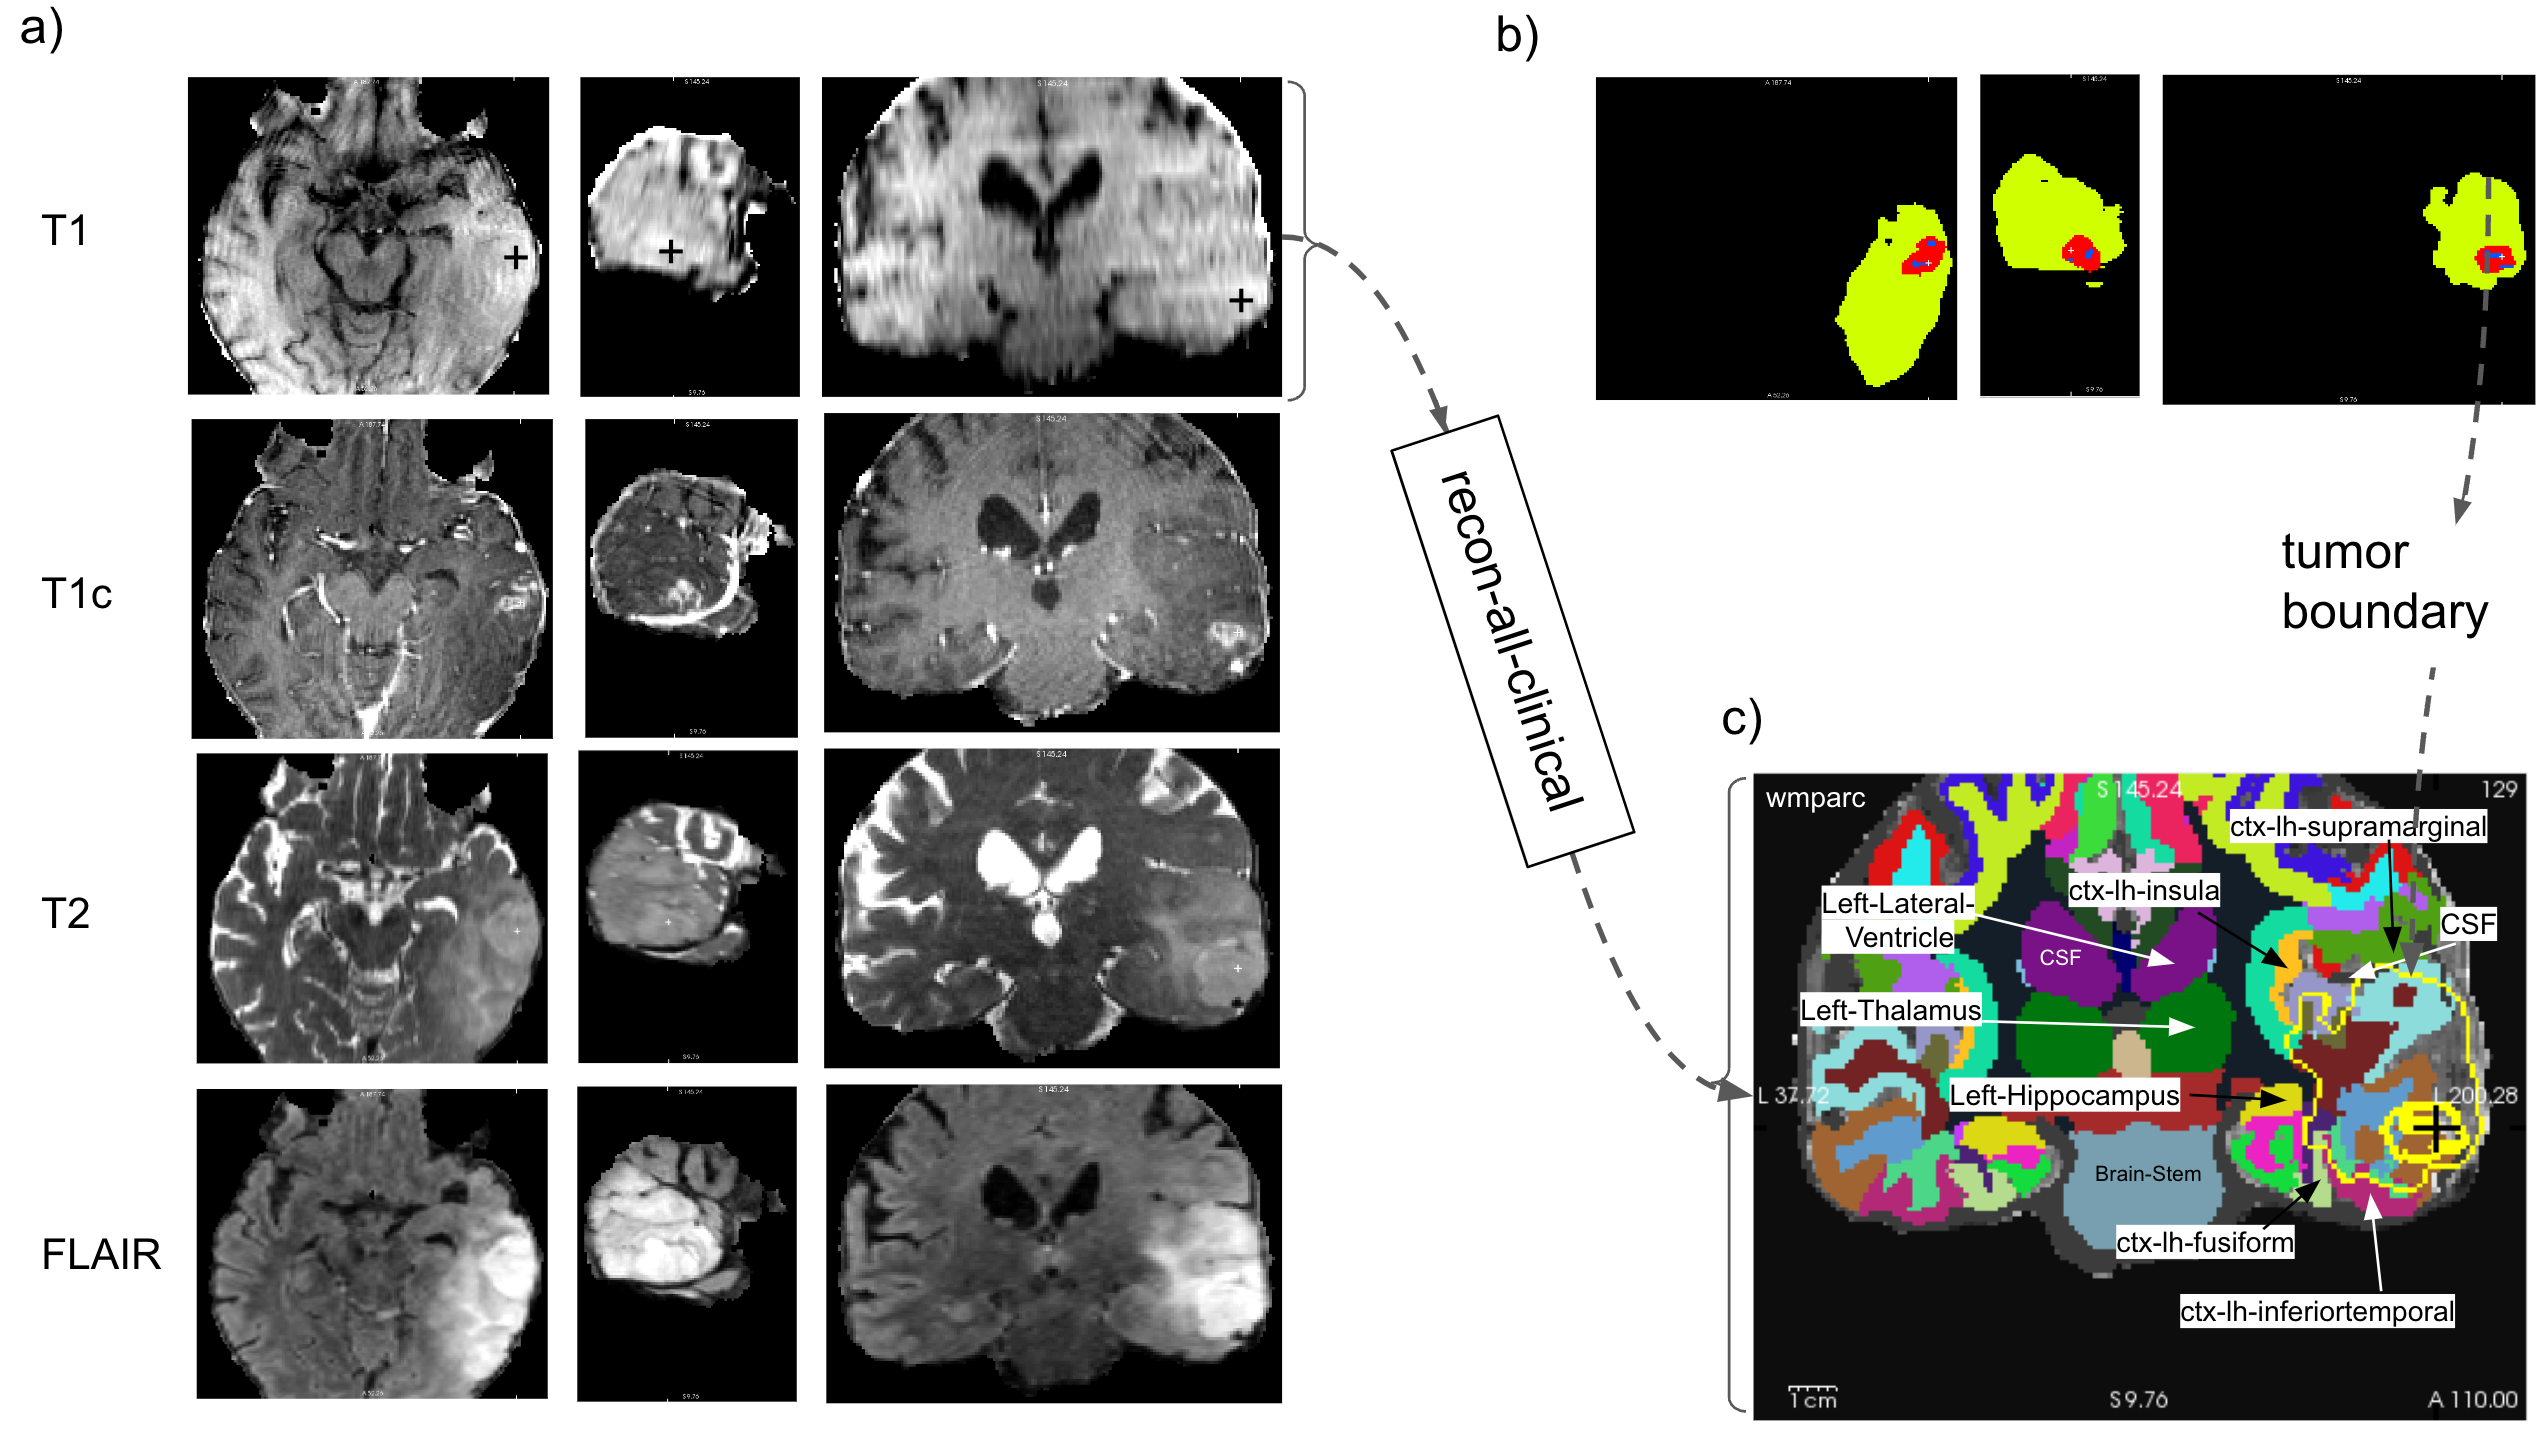
\includegraphics[width=0.92\textwidth]{figs/glioma-localization-figs-UCSF-PDGM-0085-pipeline.png}
\end{tabular}
\vspace{-1mm}
\caption{\textbf{The pipeline for anatomical tumor localization and profiling}.
a) The skull-stripped and coregistered mpMRI recording (T1, T1c, T2, FLAIR) from UCSF-PDGM-0085. The black crosshair has a center [\texttt{i=182}, \texttt{j=129}, \texttt{k=71}] (fixed for all images) located in the central part of the tumor (value 4 = ET);
b) The color-coded, three-compartment tumor segmentation mask provided by UCSF-PDGM and used as a reference mask;
c) \texttt{wmparc} segmentation. Visualization of normal and abnormal tissue in a
coronal plane shown as annotated color-coded overlays, together with the tumor compartment boundaries, using the \texttt{Freeview} interactive visualization tool
and the \texttt{FreeSurferColorLUT} lookup table.}
\label{fig:UCSF-PDGM-0085-pipeline}
\end{figure}

\vspace{-2mm}

For visual, interactive inspection of the mpMRI recordings and the
corresponding segmentations, i.e.,
{\small \texttt{mpMRI= [T1, T1c, T2, FLAIR, tumor\_segmentation, synthseg]}}, where\\
{\small \texttt{mpMRI.shape=(240,240,155,5)}}, and
for producing figures, we used \texttt{FreeView}, the data viewer provided by
\texttt{FreeSurfer}. For labeling \texttt{SynthSeg} and \texttt{wmparc} segmented regions
(cf. Figure~\ref{fig:UCSF-PDGM-0085-pipeline}), we used the\\ \texttt{FreeSurferColorLUT.txt} nomenclature for the anatomical regions
in the left and right hemispheres. For anatomical profiling we compute per-subject Hit-Plots as combinatorial voxel counts between each BraTS compartment (NCR, ED, ET) and each non-empty \texttt{wmparc} label ($172$ labels including brain-stem and CSF). Overlap volumes are reported in mL and, where noted, as fractions of intracranial volume (ICV).
For a cohort-level summary of where in the brain the leak-safe
$n=50$ UCSF-PDGM evaluation cohort sits anatomically, we bin every
\texttt{wmparc} label into 11 anatomical lobes (frontal, cingulate,
insula, parietal, temporal, occipital, sub-cortical deep,
sub-cortical limbic, cerebellum, brainstem, other) using a canonical
mapping, and aggregate the per-subject Hit-Plot CSVs by summing the
per-(label, compartment) overlap volume within each lobe. Across the
cohort, the whole-tumor compartment intersected the frontal lobe in
$90\,\%$ of subjects ($45/50$), the parietal lobe in $90\,\%$
($45/50$), the insula in $80\,\%$ ($40/50$), the sub-cortical deep
nuclei (thalamus, basal ganglia, ventral DC) in $80\,\%$ ($40/50$),
the temporal lobe in $70\,\%$ ($35/50$), the occipital lobe in
$48\,\%$ ($24/50$), the sub-cortical limbic structures (hippocampus,
amygdala) in $52\,\%$ ($26/50$), and infratentorial structures
(cerebellum and brain-stem) in $20\,\%$ ($10/50$) and $22\,\%$
($11/50$) respectively, consistent with the supratentorial-dominant
incidence distribution of adult diffuse glioma reported by
Larjavaara et~al.~\cite{Larjavaara2007}. A per-region
anatomical-profile sunburst representation is readable at the
single-subject level but aggregates poorly across the cohort. We therefore deliberately do not render the sunburst as a manuscript
figure here. Instead, the Appendix reports a compact
functional-anatomy Hit-Plot summary that keeps the analysis
descriptive: the same per-subject \texttt{wmparc} Hit-Plot CSVs are
aggregated into pre-defined label groups (lobar footprint,
motor-adjacent cortex, left language-adjacent cortex, and
deep-midline / commissural structures), with prevalence of any
overlap and median share of compartment volume reported for WT, TC,
and ET, including exploratory OS-tertile panels. These groups are
anatomical-label adjacency summaries, not tractography,
individualized eloquence mapping, fMRI, organ-at-risk proximity,
treatment-planning validation, or outcome prediction
(Discussion~\S~\emph{Limitations and translational scope},
item~(vii)).\\

\vspace{2mm}


\noindent \emph{Tumor segmentation: reference masks and the unified deep-learning engine}

\vspace{2mm}

The canonical tumour-segmentation engine for both reported
datasets is the MONAI~Bundle BraTS three-compartment SegResNet, run
behind a thin Python adapter that exposes a single
\{T1, CT1, T2, FLAIR\} $\rightarrow$ \{NCR, ED, ET\} contract on a
canonical-RAS grid. The three resulting compartments use the BraTS
label scheme (NCR$=1$, ED$=2$, ET$=4$) and are aggregated downstream
into the BraTS sub-regions WT (NCR$\,\cup\,$ED$\,\cup\,$ET),
TC (NCR$\,\cup\,$ET), and ET. The dataset-provided UCSF-PDGM masks
are retained as a per-subject \emph{reference} for the
segmentation-accuracy reporting in Table~\ref{table:dl-vs-gt}, not
as a substitute engine. For the LUMIERE longitudinal subject, two
LUMIERE-team segmentations are kept as \emph{comparators} only:
HD-GLIO-AUTO (two-compartment) and
DeepBraTumIA-native (three-compartment); their per-(timepoint,
compartment) agreement against the unified engine is reported in
Table~\ref{table:lumiere-p048-comparator-agreement}.\\

\vspace{1mm}

All processing was performed in Python~3.11 using the pinned
software stack declared in \texttt{pyproject.toml} and
\texttt{environment.yml} (NumPy, Pandas, Matplotlib, Nibabel, MONAI,
ANTsPyX, FreeSurfer~8.2.0). Deep-learning segmentation on the
$n=50$ evaluation cohort used the MONAI~Bundle 0.4.8 BraTS-3 SegResNet
backend on the stated hardware (Table~\ref{table:runtime}). The
repository and full stack are cited in \emph{Code and data availability}.



\newpage

\section{Results}

\vspace{2mm}

We first report cohort-level
segmentation accuracy of the unified MONAI~Bundle pipeline against
the UCSF-PDGM reference masks across all $n=50$ subjects
(Table~\ref{table:dl-vs-gt}), and then illustrate end-to-end
pipeline behaviour (segmentation, parcellation, anatomical
neighbourhood, and Hit-Plot) on representative cases from the
UCSF-PDGM cohort and on the LUMIERE longitudinal subject
(Patient-048). The remaining three UCSF-PDGM cases are shown in
the Appendix.

\vspace{2mm}

\noindent \emph{Quantitative segmentation accuracy on the $n=50$
UCSF-PDGM cohort}

\vspace{2mm}

The unified MONAI~Bundle BraTS three-compartment SegResNet
(Methods § \emph{Tumor segmentation}) was run on all $n=50$ subjects
of the leak-safe UCSF-PDGM evaluation cohort
(Table~\ref{table:ucsf-pdgm-cohort50}). Per-subject DL outputs were
compared against the dataset-provided tumor masks using the
operational definition of segmentation accuracy fixed in Methods §
\emph{Terminology}, sense~(i): Dice similarity coefficient, $95$th-percentile
Hausdorff distance (HD$_{95}$), absolute volumetric error
($|\mathrm{VE}|$), sensitivity and specificity, computed per BraTS
compartment (whole tumor WT, tumor core TC, enhancing tumor ET).
Cohort-level distributions are summarised as median followed by the
$[$Q1, Q3$]$ inter-quartile range in Table~\ref{table:dl-vs-gt}.
Median Dice is $0.901$, $0.941$, $0.862$ for WT, TC, ET respectively,
i.e.\ above the BraTS-2018 strict operating-point band (WT $\geq$ $0.85$,
TC $\geq$ $0.75$, ET $\geq$ $0.70$ Dice) on the cohort median. The
pre-registered outlier audit on these per-subject metrics (Methods §
\emph{Per-subject outlier audit on Table~\ref{table:dl-vs-gt}};
Limitations item~(vi)) flagged $16/50$ subjects against the same
strict band, and visual adjudication retained all sixteen.

\begin{table}[H]
\centering
\begin{tabular}{l c c c}
\toprule
Metric & WT & TC & ET \\
\midrule
Dice & 0.901 [0.850, 0.932] & 0.941 [0.900, 0.963] & 0.862 [0.793, 0.898] \\
HD$_{95}$ (mm) & 4.12 [2.45, 6.87] & 2.24 [1.00, 4.30] & 2.00 [1.41, 3.45] \\
$|\mathrm{VE}|$ (mm$^3$) & 8170 [3534, 15288] & 1385 [619, 2618] & 2430 [1065, 5741] \\
Sensitivity & 0.875 [0.784, 0.902] & 0.927 [0.864, 0.955] & 0.793 [0.729, 0.842] \\
Specificity & 1.000 [1.000, 1.000] & 1.000 [1.000, 1.000] & 1.000 [1.000, 1.000] \\
\bottomrule
\end{tabular}

\vspace{2mm}
\caption{\textbf{Per-subject segmentation accuracy of the unified
MONAI~Bundle pipeline against the UCSF-PDGM reference masks ($n=50$).}
Each cell reports the cohort-level median followed by the
$[$Q1, Q3$]$ inter-quartile range across $n=50$ subjects. WT, TC, ET
refer to the BraTS subregions (whole tumor, tumor core, enhancing
tumor). HD$_{95}$ in millimetres, $|\mathrm{VE}|$ (absolute
volumetric error) in cubic millimetres. Per-voxel specificity is reported for completeness but saturates at
$1.000$ in every cell: the denominator
$\mathrm{TN}+\mathrm{FP}$ is dominated by non-tumour brain voxels
($\sim\!10^6$ background vs.\ $\sim\!10^3$ false positives per
subject), so even substantially over-segmenting predictions round
to the same value and the metric is not discriminative for this task. Dice, HD$_{95}$, $|\mathrm{VE}|$, and sensitivity carry the
substantive comparison. The dataset-provided tumor
masks are treated as a \emph{reference} rather than ground truth
(Limitations item~(vi); the worst-case cross-segmenter
boundary-disagreement exemplar sub-0396 is discussed there).}
\label{table:dl-vs-gt}
\end{table}

\vspace{2mm}

\subsection*{Per-pipeline-stage runtime on stated hardware}

Wall-clock runtime for the two computational stages of the
unified pipeline, measured on the same Apple~Silicon host that
processed the $n=50$ evaluation cohort, is summarised in
Table~\ref{table:runtime}. The MONAI~Bundle BraTS-3 SegResNet stage
runs in $\approx\!1.3$\,s per subject on the steady-state path
(Metal Performance Shaders, MPS), with a one-time first-call latency
of $\approx\!22$\,s per process for model-weight loading and
MPS-context initialisation. The FreeSurfer
\texttt{recon-all-clinical} anatomical parcellation stage runs
single-host, multi-threaded on CPU and is the dominant contributor
to total cohort runtime. Per-subject elapsed time is captured as a
structured field in every per-subject sidecar so the table is fully
regenerable from the on-disk derivatives, with a per-subject audit
CSV and a JSON companion that records the host fingerprint. The
pinned software stack and repository are cited in \emph{Code and data
availability}.

\begin{table}[H]
\centering
\begingroup\small
\begin{tabularx}{\textwidth}{>{\raggedright\arraybackslash}X >{\raggedright\arraybackslash}X l c >{\raggedright\arraybackslash}X}
\toprule
Stage & Backend & Device & $n$ & Wall-clock per subject (median [Q1, Q3]) \\
\midrule
DL segmentation (first-call latency) & MONAI Bundle 0.4.8 (BraTS-3 SegResNet) & MPS & 1 & 22.01\,s \\
DL segmentation (steady-state) & MONAI Bundle 0.4.8 (BraTS-3 SegResNet) & MPS & 49 & 1.29\,s [1.28\,s, 1.35\,s] \\
Anatomical parcellation & FreeSurfer 8.2.0 recon-all-clinical (wmparc) & CPU/10t & 50 & 35:25\,min [32:38\,min, 41:08\,min] \\
\bottomrule
\end{tabularx}
\endgroup

\vspace{2mm}
\caption{\textbf{Per-pipeline-stage wall-clock runtime on stated
hardware ($n=50$ evaluation cohort).} Auto-generated from the
per-subject elapsed-time fields in the on-disk derivatives. The DL
segmentation stage is split into a single
``first-call latency'' row (cold-start cost paid once per process
for MONAI~Bundle weight loading and MPS-context initialisation) and
a ``steady-state'' row (the remaining $n{-}1$ subjects). Cells
report median followed by the $[$Q1, Q3$]$ inter-quartile range,
auto-formatted as seconds, MM:SS, or HH:MM:SS depending on
magnitude. The $n$ column reports cells where data are present out
of the cohort total ($n_{\text{used}}/n_{\text{expected}}$ when
different); a partial-cohort denominator on the parcellation row
indicates that the long-running FreeSurfer fan-out was still in
flight when this table was last regenerated. Re-running the runtime
benchmark after the fan-out completes refreshes all cells in
place.}
\label{table:runtime}
\end{table}

\vspace{2mm}

\subsection*{Spatial-pattern agreement: Hit-Plot panel
(DL vs UCSF-PDGM reference)}

Spatial-pattern agreement between the unified DL pipeline
and the dataset-provided reference masks was assessed on a
per-(subject, anatomical region, BraTS compartment) basis using
the Hit-Plot regional-tumor-burden representation
(Methods § \emph{Methods for anatomical tumor localization and profiling}). With the FreeSurfer
\texttt{recon-all-clinical} parcellation acting as the
binning grid, every cell encodes the percentage of one parcel
occupied by one BraTS compartment, in one subject. Across all
$n=50$ subjects $\times$ $172$ wmparc regions $=$ $8\,600$ cells
per compartment, the concordance correlation coefficient (CCC)
between DL and reference is $0.974$ (WT), $0.992$ (TC), and
$0.951$ (ET); mean differences are $-0.53$, $-0.07$, and $-0.24$
percentage points of the underlying parcel volume, with $95$\%
Bland-Altman limits of agreement $[-7.73, +6.67]$ (WT),
$[-2.20, +2.06]$ (TC), and $[-3.47, +2.99]$ (ET) percentage
points; mean absolute volumetric differences per cell are
$80.9$, $17.1$, and $25.3$~mm$^3$, respectively.
Figure~\ref{fig:hitplot-agreement} renders the per-compartment
Bland-Altman scatter against the cell-mean.

Beyond the volumetric Hit-Plot reported here, the pipeline also
computes a probabilistic Hit-Plot that propagates the segmenter's
per-class sigmoid probabilities into a per-cell Poisson-binomial mean and standard
deviation. These per-subject outputs are produced by the released
build chain, and a dedicated analysis of the propagated per-cell
uncertainty is beyond the scope of the present feasibility report.

\begin{figure}[H]
\centering
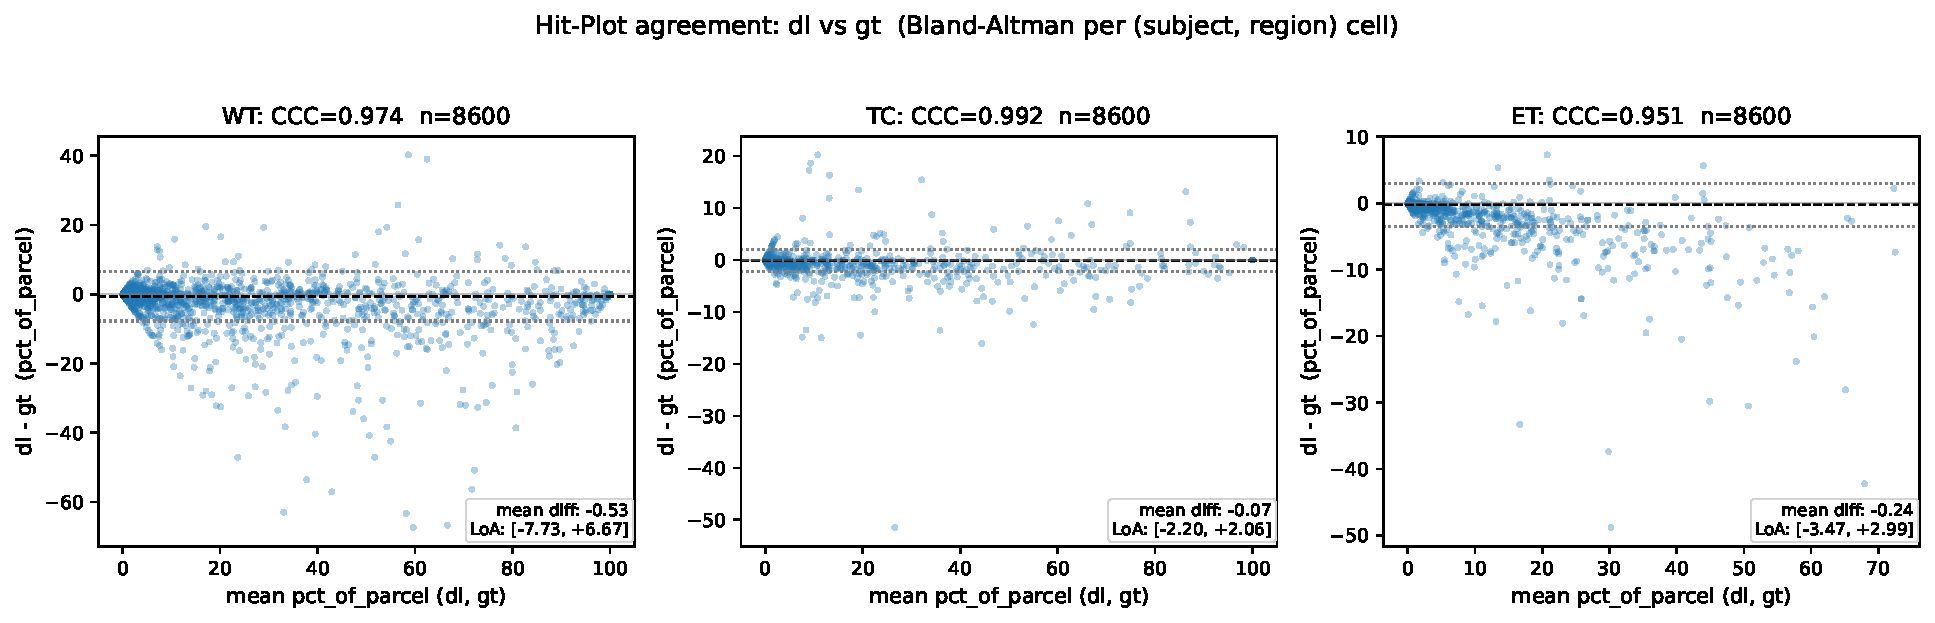
\includegraphics[width=\linewidth]{figs/fig_hitplot_agreement_dl_vs_gt.pdf}
\caption{\textbf{Cell-level spatial-pattern agreement between
the unified DL pipeline and the UCSF-PDGM reference masks
($n=50$ cohort, $172$ wmparc regions, three BraTS compartments;
$8\,600$ cells per compartment).}
Each panel is a Bland-Altman scatter of the per-(subject,
region) Hit-Plot cell value (percentage of the parcel occupied
by the BraTS compartment) for one compartment (WT, TC, ET).
Solid horizontal line: cohort mean difference
($-0.53$, $-0.07$, $-0.24$ pp for WT, TC, ET);
dashed lines: $95$\% limits of agreement
(mean $\pm 1.96\,\sigma_{\text{diff}}$;
$[-7.73, +6.67]$, $[-2.20, +2.06]$, $[-3.47, +2.99]$ pp).
Concordance correlation coefficient (CCC; $0.974$, $0.992$,
$0.951$) and mean absolute volumetric difference per cell
($|\Delta V|$; $80.9$, $17.1$, $25.3$~mm$^3$) are reported in the
panel headers. The companion audit CSV and machine-readable summary
sidecar are archived alongside the figure (cf.\ \emph{Code and data
availability}).}
\label{fig:hitplot-agreement}
\end{figure}

\vspace{2mm}

\subsection*{Functional-anatomy summary of the Hit-Plot}

To make the per-region Hit-Plot representation readable at the
cohort level without claiming individualized functional mapping, we
also aggregate the same $n=50$ \texttt{wmparc} Hit-Plot CSVs into
pre-defined anatomical-label groups (Appendix~4,
Figure~\ref{fig:functional-anatomy-hitplot}). The whole-tumor (WT)
compartment intersects motor-adjacent labels in $44/50$ subjects
($88\,\%$), with a median $7.97\,\%$ of WT volume falling in that
group; left language-adjacent labels in $27/50$ subjects ($54\,\%$),
median $0.79\,\%$ of WT volume; and deep-midline / commissural labels
in $40/50$ subjects ($80\,\%$), median $1.72\,\%$ of WT volume. The
same producer run on Hit-Plot-DL yields similar descriptive summaries
(motor-adjacent WT $43/50$, median $6.91\,\%$; left
language-adjacent WT $27/50$, median $0.71\,\%$; deep-midline /
commissural WT $42/50$, median $2.06\,\%$), consistent with the
cell-level DL-vs-reference agreement in
Figure~\ref{fig:hitplot-agreement}. A bounded \texttt{mri\_TumorSynth}
segmentation-backbone sensitivity run on the same $n=50$ staged
inputs gives the same qualitative functional-anatomy pattern
(Appendix~5): motor-adjacent WT $43/50$, median $6.27\,\%$; left
language-adjacent WT $27/50$, median $0.84\,\%$; and deep-midline /
commissural WT $41/50$, median $1.28\,\%$. These values are presented as an
appendix-level anatomical readability check of the Hit-Plot variants,
not as tractography, functional eloquence mapping, treatment-planning
validation, or outcome prediction. The OS-tertile panels in
Figure~\ref{fig:functional-anatomy-hitplot} demonstrate only that the
same descriptive summaries can be stratified by available clinical metadata. They are not a test of regional-burden/outcome association.

\vspace{2mm}

\noindent \emph{Cases from the UCSF-PDGM dataset}

\vspace{2mm}

We illustrate end-to-end pipeline behaviour on five \emph{illustrative}
UCSF-PDGM detail subjects (Methods, Table~\ref{table:ucsf-pdgm-subjects};
not the $n=50$ evaluation cohort). The pipeline is individually evaluated
and visually assessed with a detailed, interactive inspection of the
original recordings, the co-registered tumor masks (used as a reference),
and the normal tissue segmentation masks from \texttt{FreeSurfer},
including \texttt{SynthSeg}.

Figure~\ref{fig:UCSF-PDGM-0020_a_h} shows the segmentation results for a single subject (id=0020).
The segmentations and tumor localization profiles (``Hit-Plots'') for this and subject (id=0022)
are shown in Figures~\ref{fig:UCSF-PDGM-0020_countouring}, \ref{fig:UCSF-PDGM-0022_countouring}, respectively;
the corresponding figures for the three appendix subjects (id=0039, 0066, 0085) are
Figures~\ref{fig:UCSF-PDGM-0039_countouring}, \ref{fig:UCSF-PDGM-0066_countouring}, \ref{fig:UCSF-PDGM-0085_countouring}.
The bar-chart bottom half of each per-subject figure (panel~c of Figures~\ref{fig:UCSF-PDGM-0020_countouring}, \ref{fig:UCSF-PDGM-0022_countouring}, \ref{fig:UCSF-PDGM-0039_countouring}, \ref{fig:UCSF-PDGM-0066_countouring}, \ref{fig:UCSF-PDGM-0085_countouring}) is computed from the FreeSurfer~8.2.0 \texttt{recon-all-clinical} \texttt{wmparc} parcellation. Bars are stacked NCR (red, label~1) $+$ ED (green, label~2) $+$ ET (yellow, label~4); their sum equals the whole-tumor volume in each region, and per-region totals (mL) are annotated to the right of each bar (NCR $=$ Necroses, non-enhancing tumor; ED $=$ FLAIR abnormality, edema compartment; ET $=$ Enhancing tumor). These five detail subjects are leak-unsafe for our DL engine by construction (four of five sit in the BraTS21 Segmentation Training cohort and the fifth in Validation), so the per-subject Hit-Plot bars in the main text are reference-mask-based; the supplementary 5\,$\times$\,1 DL-vs-reference panel of APPENDIX~3 (Figure~\ref{fig:supp-legacy5-dlvsgt}) demonstrates per-subject DL-vs-reference agreement on five representative subjects from the leak-safe $n=50$ evaluation cohort.

\begin{figure}[H]
\begin{tabular}{cc}
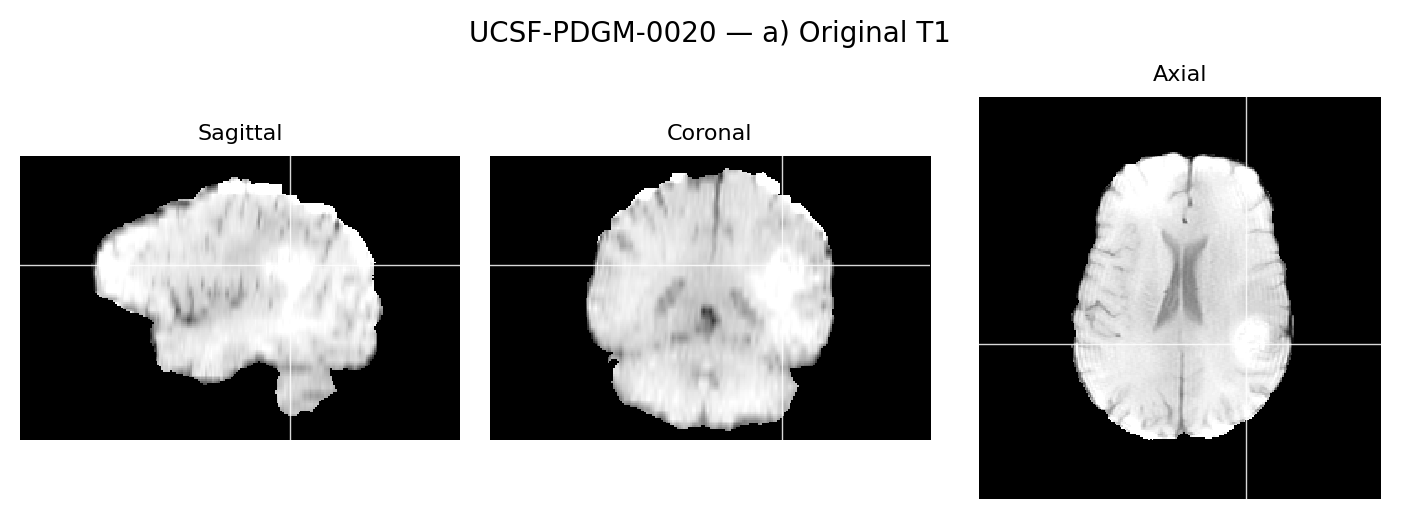
\includegraphics[width=0.48\textwidth]{figs/glioma-localization-figs-UCSF-PDGM-0020_panel_a.png} &
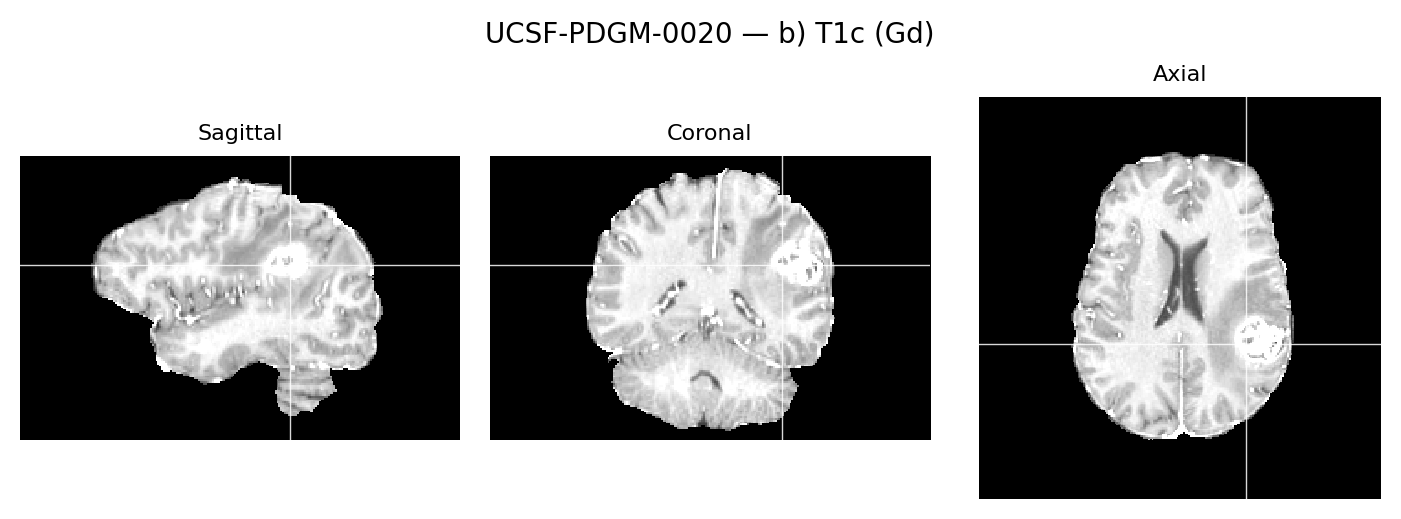
\includegraphics[width=0.48\textwidth]{figs/glioma-localization-figs-UCSF-PDGM-0020_panel_b.png} \\
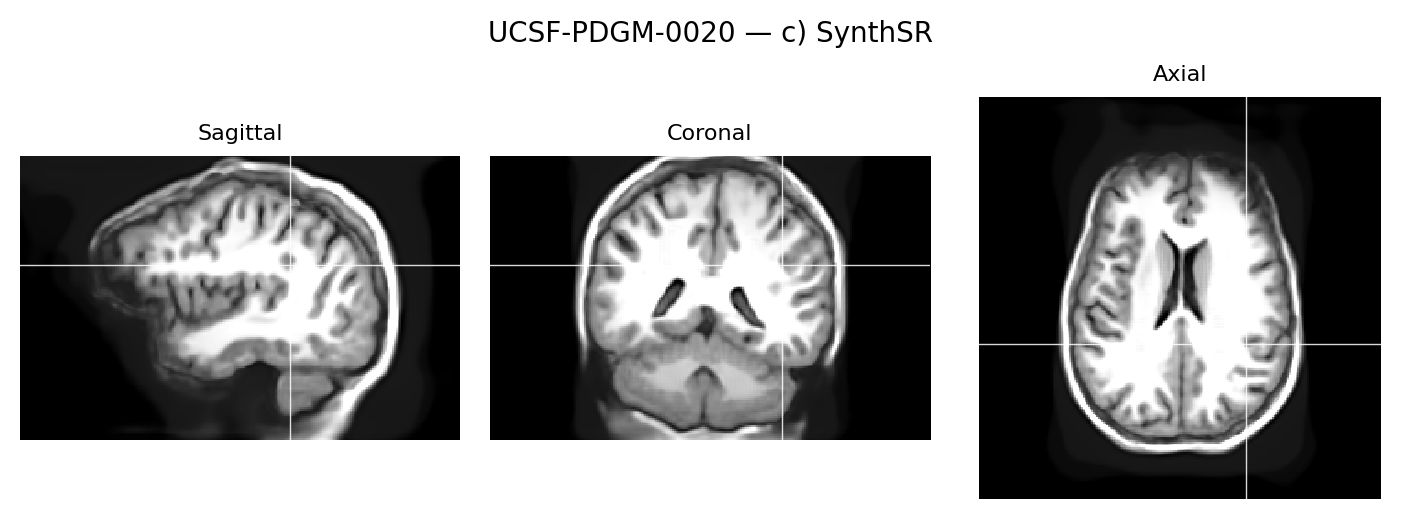
\includegraphics[width=0.48\textwidth]{figs/glioma-localization-figs-UCSF-PDGM-0020_panel_c.png} &
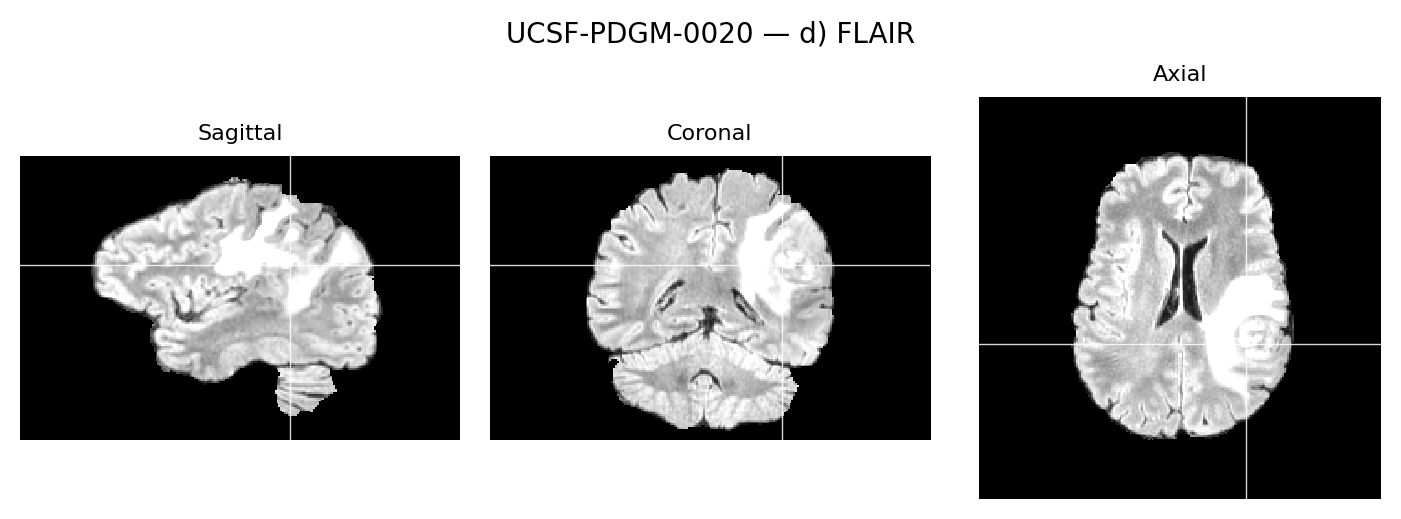
\includegraphics[width=0.48\textwidth]{figs/glioma-localization-figs-UCSF-PDGM-0020_panel_d.png} \\
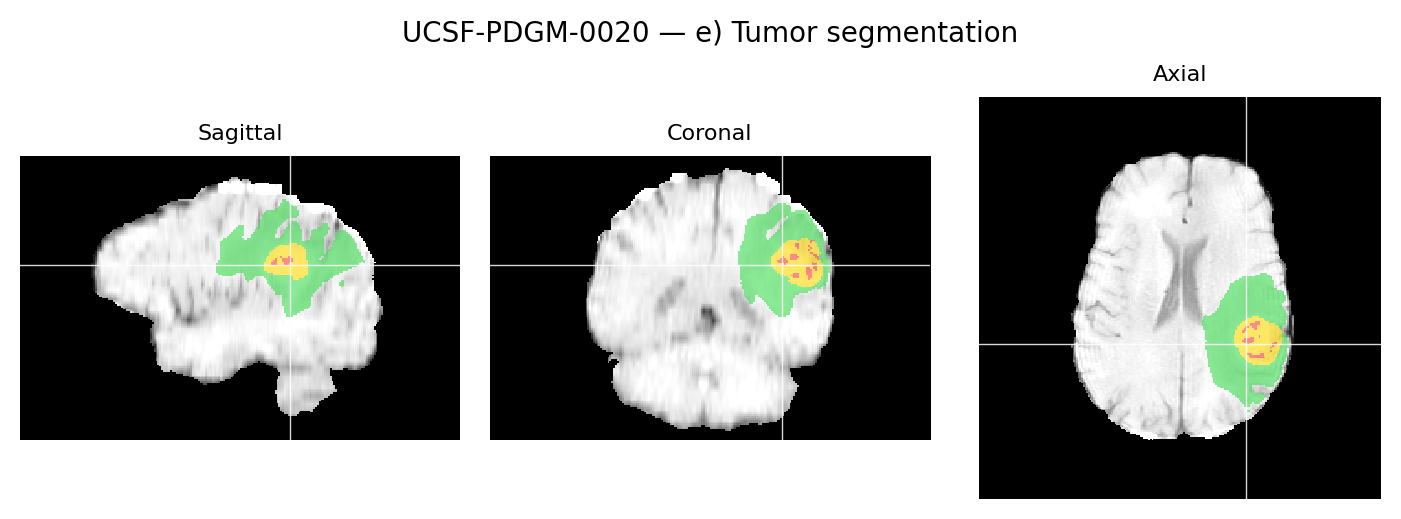
\includegraphics[width=0.48\textwidth]{figs/glioma-localization-figs-UCSF-PDGM-0020_panel_e.png} &
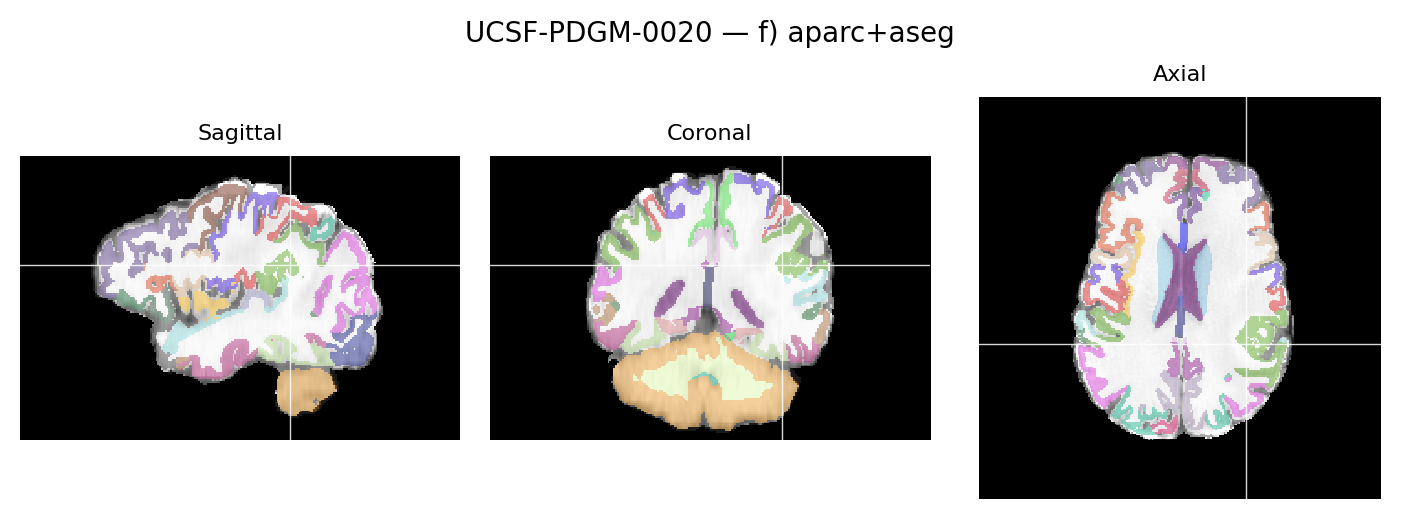
\includegraphics[width=0.48\textwidth]{figs/glioma-localization-figs-UCSF-PDGM-0020_panel_f.png} \\
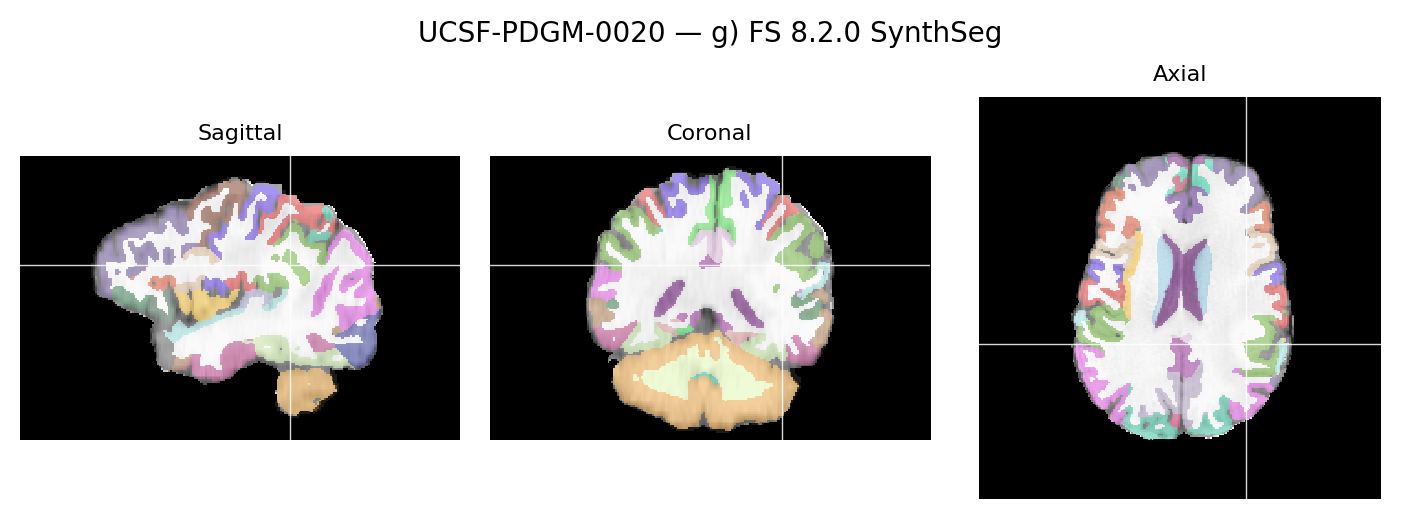
\includegraphics[width=0.48\textwidth]{figs/glioma-localization-figs-UCSF-PDGM-0020_panel_g.png} &
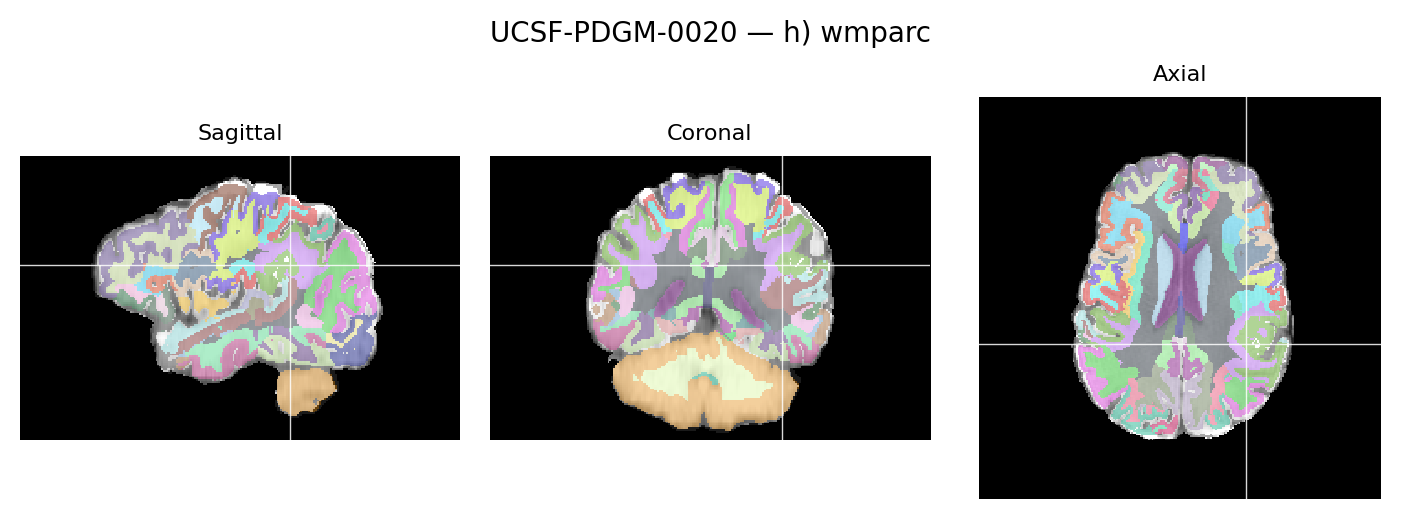
\includegraphics[width=0.48\textwidth]{figs/glioma-localization-figs-UCSF-PDGM-0020_panel_h.png}
\end{tabular}
\caption{\textbf{Segmentation of tumor (provided by the UCSF-PDGM team) and probable underlying anatomical regions in study UCSF-PDGM-0020}. All eight panels are produced end-to-end with the unified HPGS pipeline: \texttt{mri\_synthsr} produces the super-resolution T1; \texttt{recon-all-clinical.sh} (FreeSurfer~8.2.0) produces \texttt{aparc+aseg} and \texttt{wmparc}; and \texttt{mri\_synthseg --robust --parc} produces the SynthSeg parcellation. The FS outputs are resampled back to the native mpMRI grid with \texttt{mri\_convert -rl} for voxel-aligned display. All panels are displayed in the conventional \emph{radiological} orientation on canonical-RAS data (image-left $=$ patient-right for the axial and coronal planes; anterior-left for the sagittal plane; superior up for the axial and sagittal planes).
a) Original T1. The black crosshair is fixed at [\texttt{i=159}, \texttt{j=147}, \texttt{k=95}] in all panels and is centred in the tumor;
b) Original Gadolinium-contrast enhanced T1-weighted image (T1c);
c) SynthSR~\cite{Iglesias2023} super-resolution 1\,mm MPRAGE synthesised from the original T1;
d) Original FLAIR image;
e) Three-compartment tumor segmentation mask (NCR=1, ED=2, ET=4) overlaid on the bias-corrected T1 used by HPGS;
f) \texttt{aparc+aseg} from \texttt{recon-all-clinical.sh};
g) FreeSurfer 8.2.0 \texttt{SynthSeg} parcellation from the same subject's T1;
h) \texttt{wmparc} from \texttt{recon-all-clinical.sh}. Color-coded label overlays follow the \texttt{FreeSurferColorLUT} lookup table.}
\label{fig:UCSF-PDGM-0020_a_h}
\end{figure}

\begin{figure}[H]
\begin{tabular}{c}
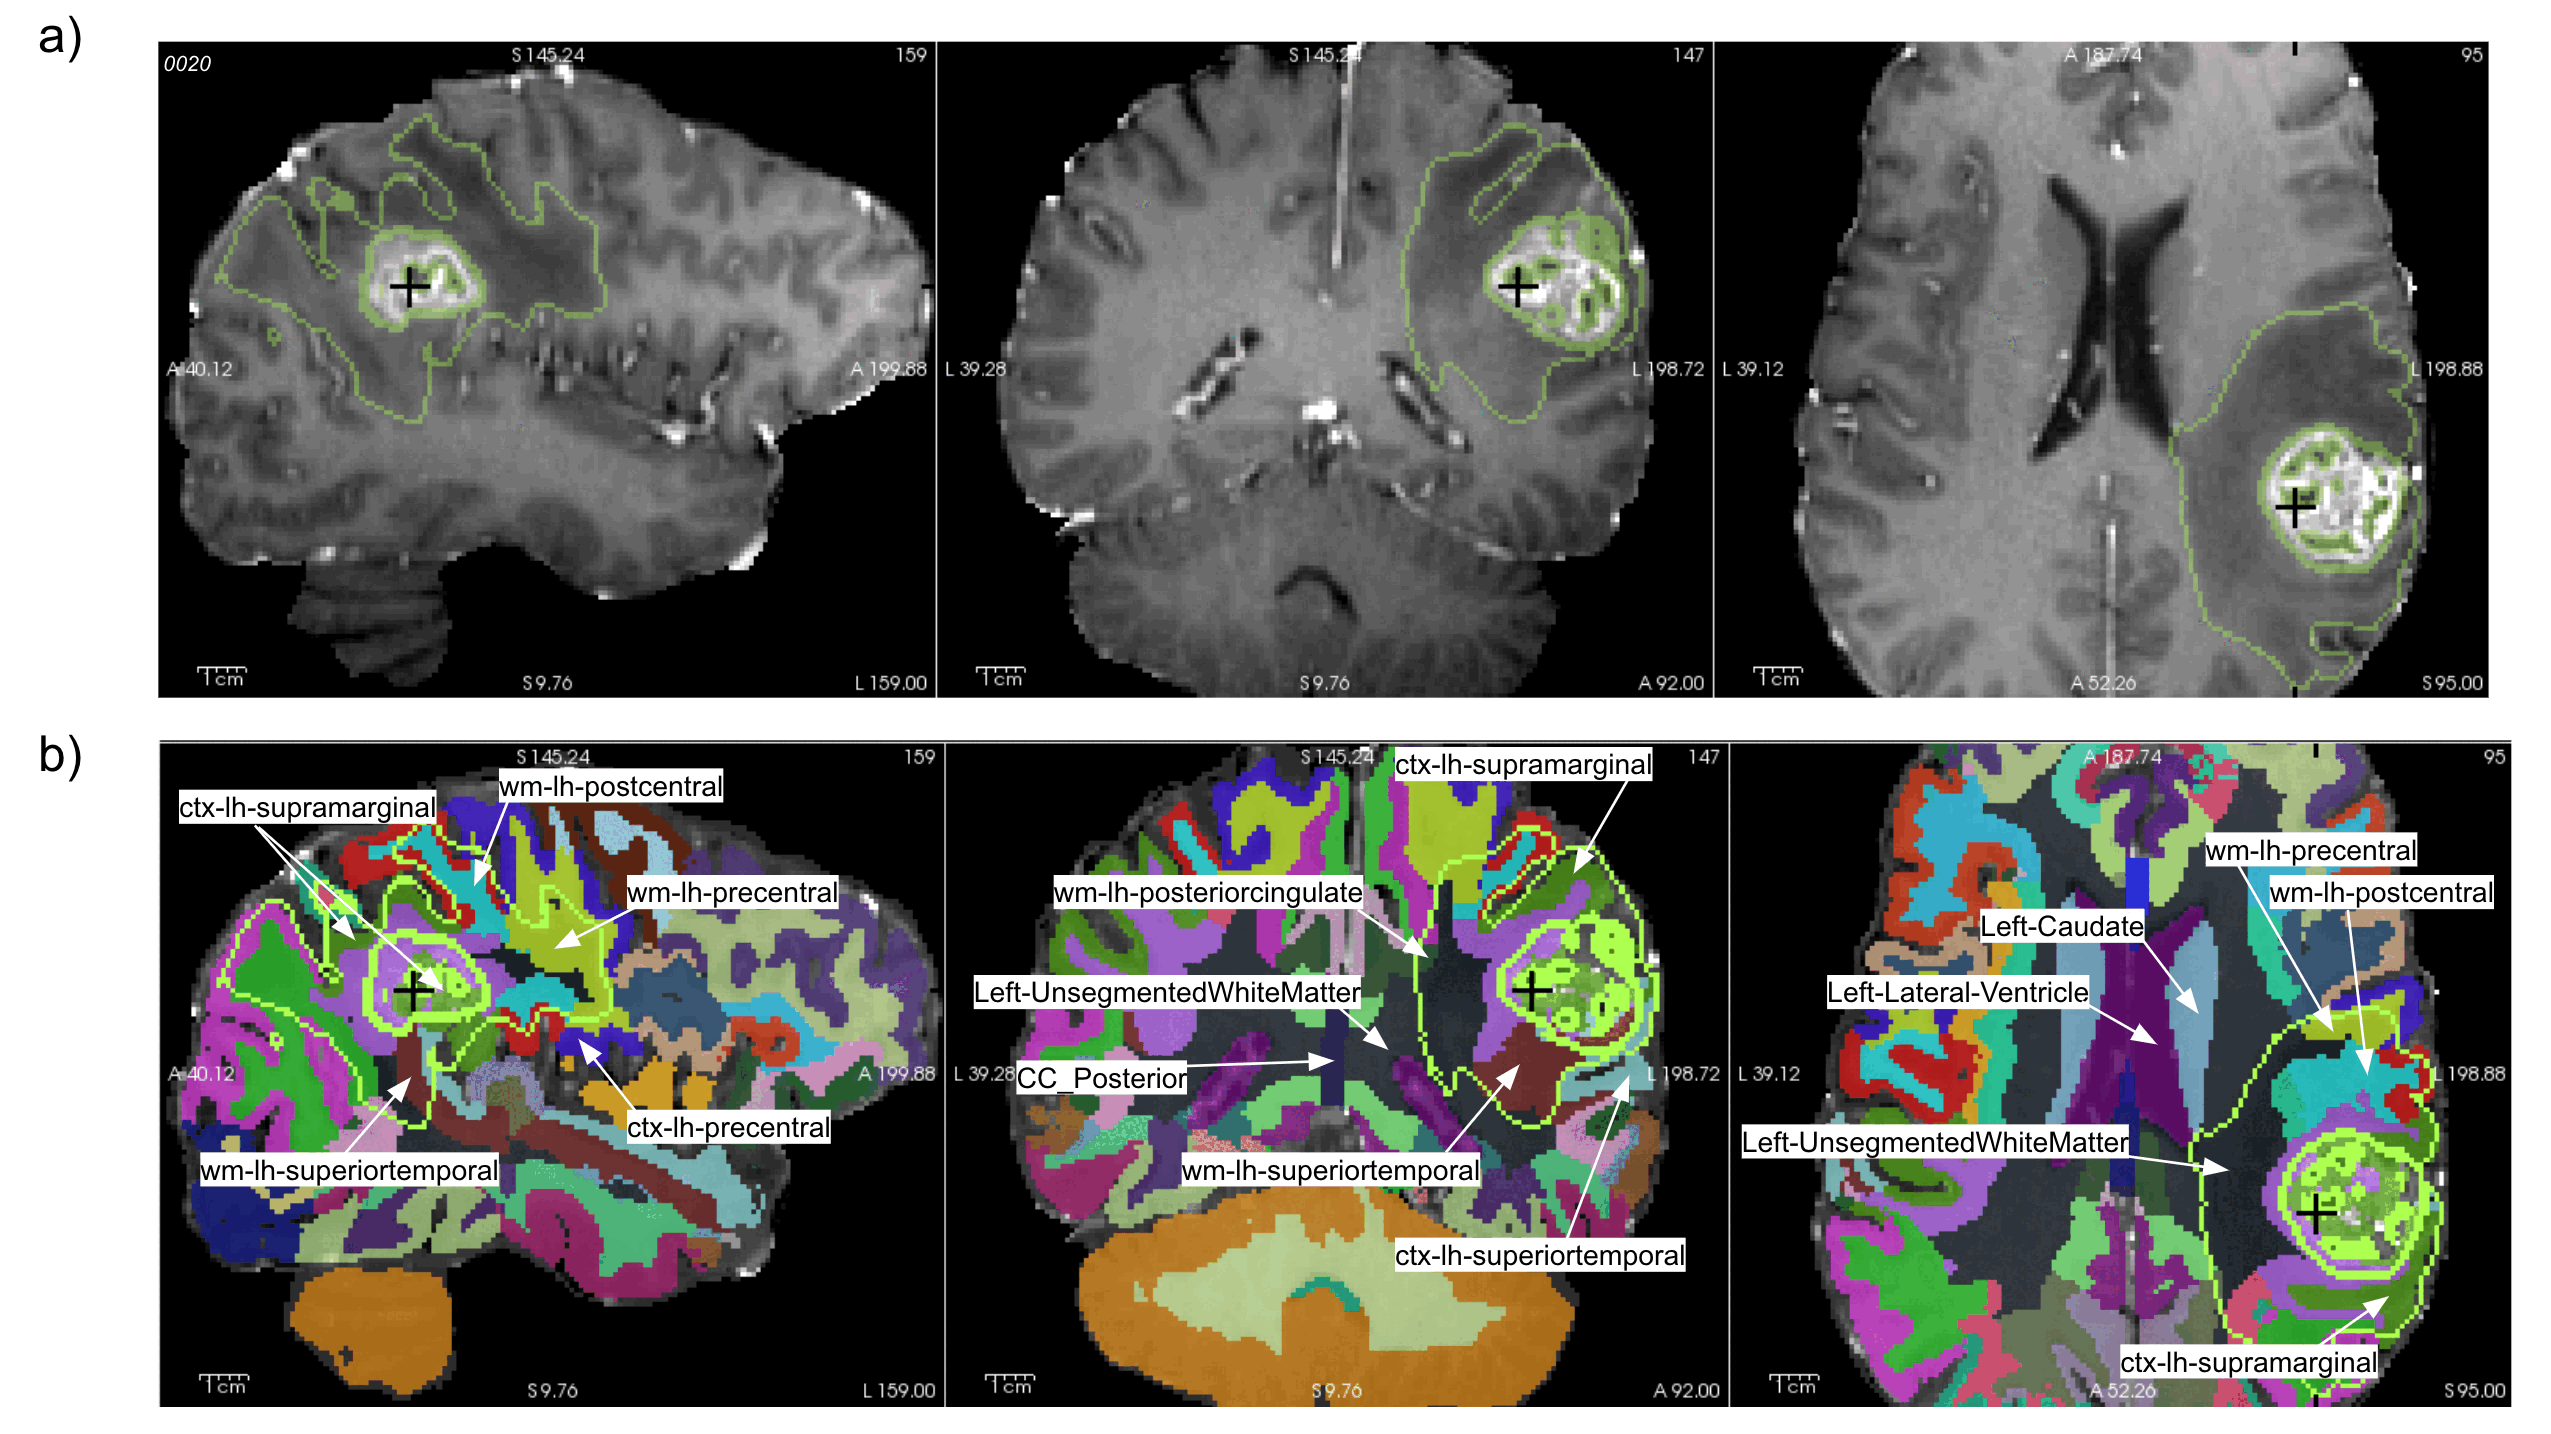
\includegraphics[width=0.92\textwidth]{figs/glioma-localization-figs-UCSF-PDGM-0020-tumor-contours-on-wmparc.png} \\
\vspace{-2mm}
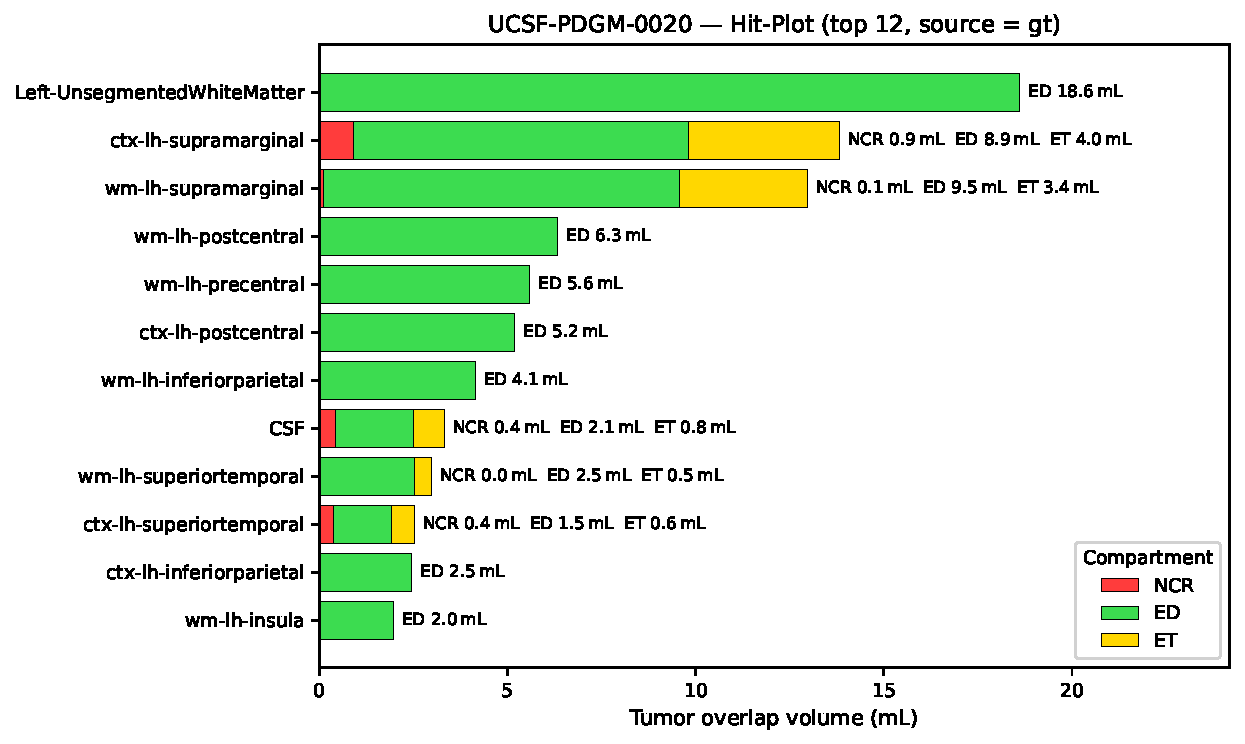
\includegraphics[width=0.80\textwidth]{figs/sub-0020_panel_i_hitplot_gt.pdf}
\end{tabular}
\vspace{-2mm}
\caption{\textbf{Tumor location and anatomical neighborhoods from the study UCSF-PDGM-0020.}\\ a) The original Gadolinium-contrast enhanced T1-weighted image (T1c) with an overlay of tumor region boundaries. b) The \texttt{wmparc} segmentation with an overlay of tumor compartment boundaries and annotation of selected anatomical structures and regions in the tumor surroundings. The black crosshair center is located at [\texttt{i=159}, \texttt{j=147}, \texttt{k=95}]. Visualization of normal and abnormal tissue in the sagittal, coronal, and axial planes are made with \texttt{Freeview} and color-coded labels according to the \texttt{FreeSurferColorLUT} lookup table. \\c) Tumor compartment ``Hit-Plot'' for the top-12 \texttt{wmparc} parcels of this subject.}
\label{fig:UCSF-PDGM-0020_countouring}
\end{figure}


\begin{figure}[H]
\begin{tabular}{c}
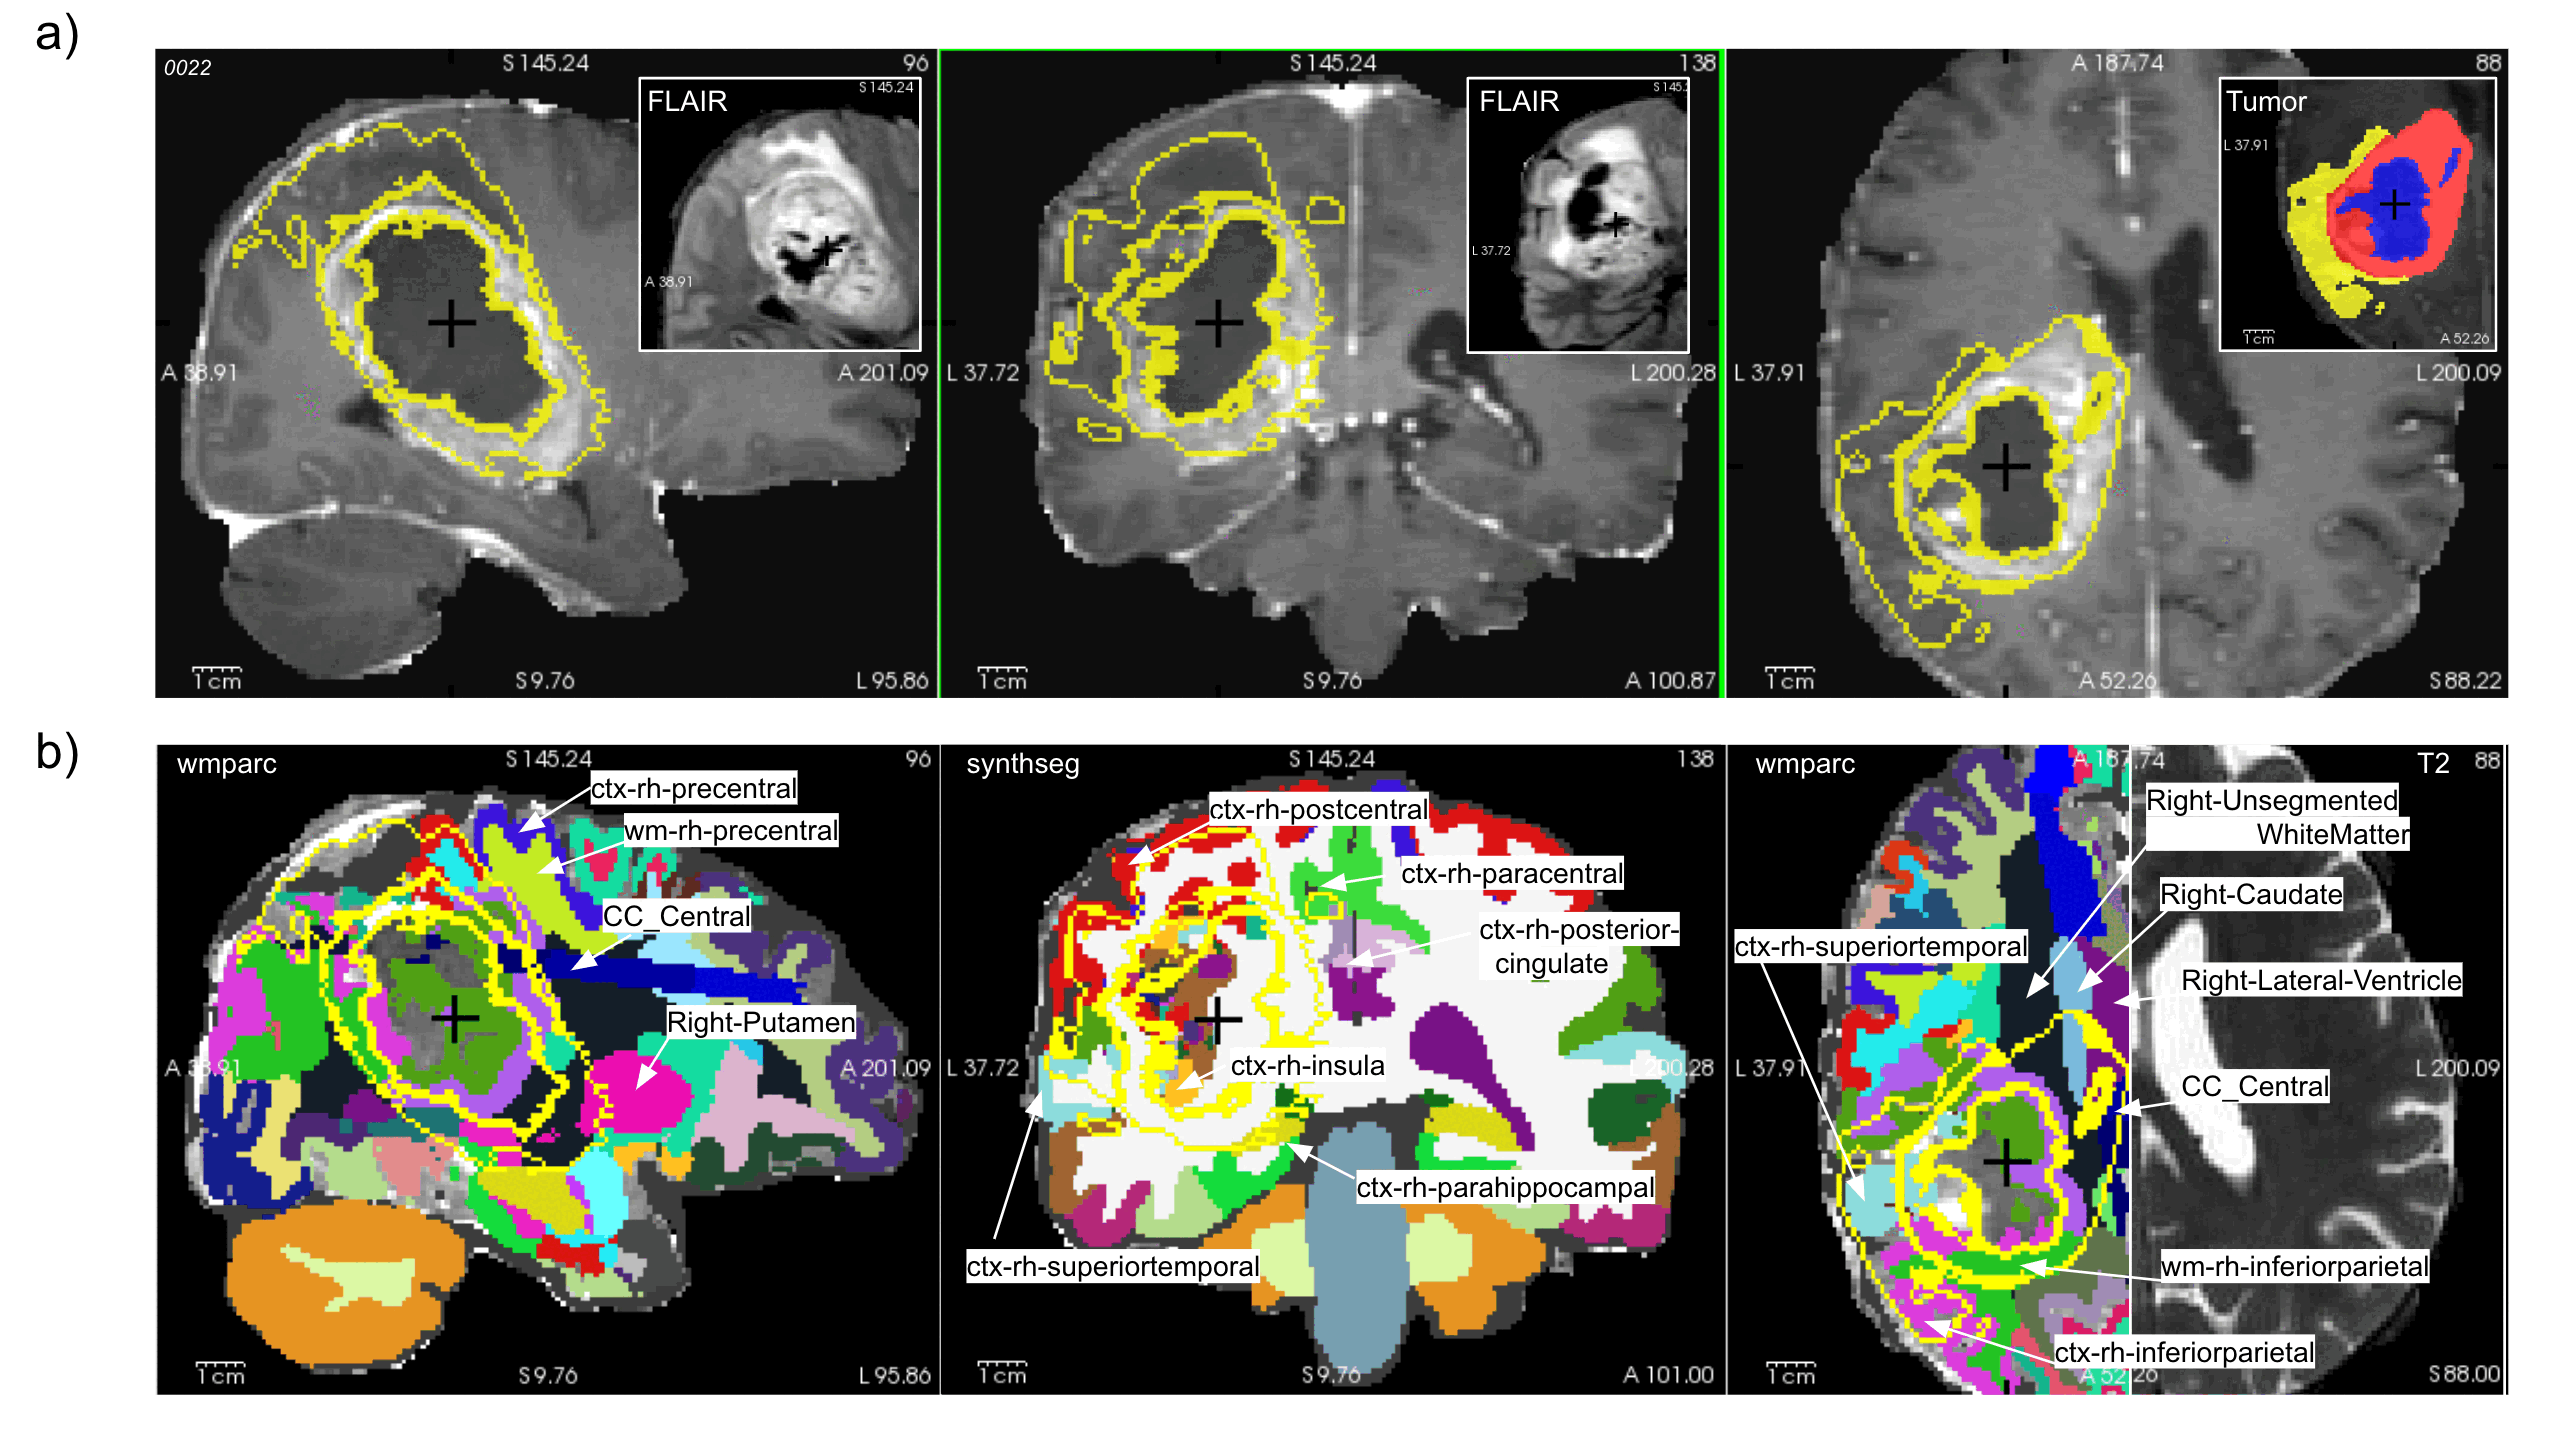
\includegraphics[width=0.70\textwidth]{figs/glioma-localization-figs-UCSF-PDGM-0022-tumor-contours-on-wmparc.png} \\
\vspace{-2mm}
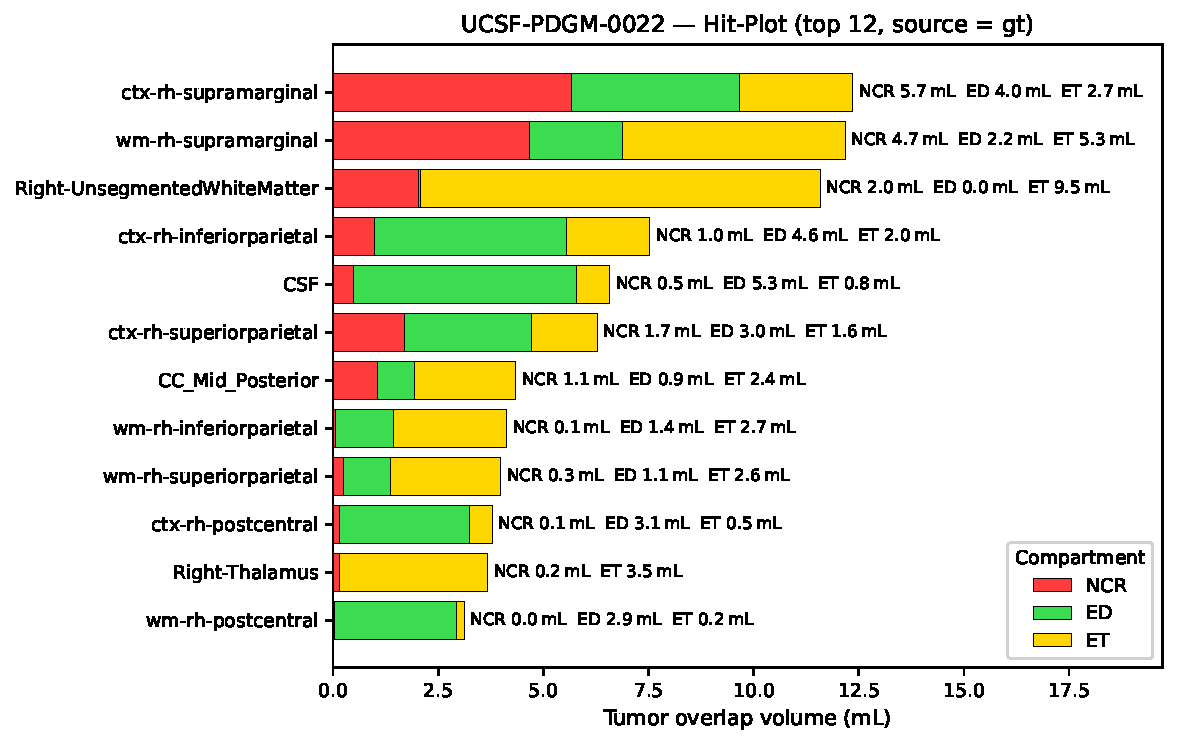
\includegraphics[width=0.64\textwidth]{figs/sub-0022_panel_i_hitplot_gt.pdf}
\end{tabular}
\vspace{-4mm}
\caption{\textbf{Tumor location and anatomical neighborhoods from the study UCSF-PDGM-0022.}\\ a) The original Gadolinium-contrast enhanced T1-weighted image (T1c) with an overlay of tumor region boundaries. Inserts covering the tumor region in the left and middle panel show the corresponding FLAIR channel. Insert in the right panel shows the corresponding three-compartment tumor segmentation using our extended \texttt{FreeSurferTumorColorLUT} lookup table. b) The \texttt{wmparc} segmentation with an overlay of tumor compartment boundaries and annotation of selected anatomical structures and regions in the tumor surroundings. In the right panel, the left hemisphere (not containing the segmented tumor) is shown as the T2 channel. The black crosshair center is located at [\texttt{i=96}, \texttt{j=138}, \texttt{k=88}]. Visualization of normal and abnormal tissue in the sagittal, coronal, and axial planes are made with \texttt{Freeview} and color-coded labels according to the \texttt{FreeSurferColorLUT} lookup table. c) Tumor compartment ``Hit-Plot'' for the top-12 \texttt{wmparc} parcels of this subject.}
\label{fig:UCSF-PDGM-0022_countouring}
\end{figure}


\newpage

\noindent \emph{One case from the LUMIERE dataset with longitudinal examinations}

\vspace{2mm}

We process all six mpMRI examinations of Patient-048 in the
LUMIERE collection (cf.\ Figure~\ref{fig:Suter2022_fig2}) under the
unified evaluation framework: per-timepoint rigid coregistration into
a single pre-operative reference space (Methods~\S~\emph{The LUMIERE
dataset}), then per-timepoint segmentation by the unified
MONAI~Bundle BraTS three-compartment SegResNet on the registered
\{T1,~CT1,~T2,~FLAIR\} stack. The resulting BraTS three-compartment
trajectory (NCR, ED, ET, plus the derived TC$=$NCR$+$ET and
WT$=$NCR$+$ED$+$ET) is shown in
Figure~\ref{fig:fig6-lumiere-p048-volumes}, on a continuous
day-resolved time axis with the LUMIERE-anonymisation disclosure
propagated into the caption. Quantitatively, the trajectory recovers
the expected RANO-aligned dynamics for this subject: a maximal-tumour
pre-operative scan (WT $=140.1$\,mL, ET $=24.0$\,mL at day~0), a
post-operative drop in enhancing tumour (ET $=3.7$\,mL at day~3, a
$\sim\!85\%$ reduction), a mid-treatment trough at week-013 (SD;
ET $=0.7$\,mL, WT $=31.5$\,mL) followed by a CR plateau at week-023
(ET $=1.0$\,mL), and a clear recurrence by week-049 (PD;
ET $=22.7$\,mL, WT $=100.0$\,mL).

Agreement between the unified-engine segmentation and the two
LUMIERE-team reference segmentations (HD-GLIO-AUTO and the native
CT1-grid DeepBraTumIA mask, both warped through the same per-timepoint
rigid transform) is summarised compartment-by-compartment in
Table~\ref{table:lumiere-p048-comparator-agreement}. Two qualitative
patterns are worth noting. (a)~Whole-tumour (WT) and tumour-core (TC)
agreement against DeepBraTumIA is consistently high at the
high-burden timepoints (WT~Dice $0.85$ pre-op, $0.86$ post-op, $0.90$
at week-049; TC~Dice $0.95$, $0.72$, $0.92$ at the same three
timepoints) and degrades, as expected, at the low-burden CR/SD
mid-trajectory where the absolute number of tumour voxels is small
and the Dice denominator becomes noise-sensitive. (b)~Enhancing-tumour
(ET) Dice tracks the absolute ET volume rather than segmenter
identity: it is high when ET is genuinely present
(${\rm Dice} \geq 0.77$ at the pre-op and PD scans for both
comparators) and collapses when ET essentially vanishes
(${\rm Dice} \leq 0.13$ at week-000-2 / week-013 / week-023, where
the ET volume is below $\sim\!4$\,mL across all three segmenters and
HD-GLIO-AUTO in particular reports near-zero ET). This is a
volume-floor artefact of the Dice metric, not a discrepancy in the
underlying clinical reading: all three engines agree, on these three
timepoints, that there is essentially no enhancing tumour.

\begin{figure}[H]
\begin{tabular}{c}
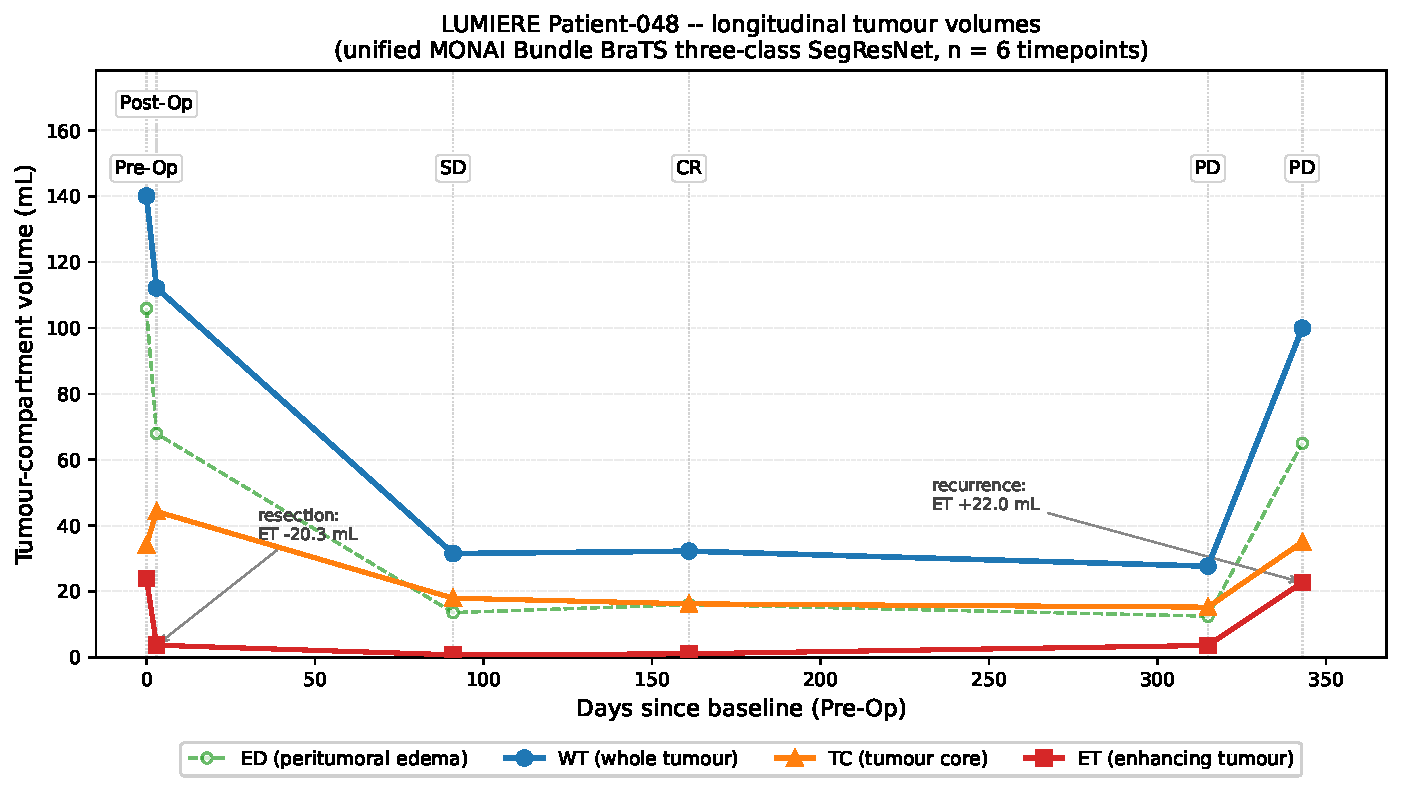
\includegraphics[width=0.99\textwidth]{figs/fig6_lumiere_p048_volumes.pdf}
\end{tabular}
\caption{\textbf{LUMIERE Patient-048 -- longitudinal tumour
volumes from the unified MONAI~Bundle BraTS three-compartment
SegResNet ($n=6$ timepoints).} Per-compartment volume (mL) on a
continuous day-resolved time axis: enhancing tumour (ET, red),
necrotic core (NCR, blue), tumour core (TC = NCR + ET, dashed),
edema (ED, green), and whole tumour (WT = NCR + ED + ET, black).
RANO labels (Pre-Op, Post-Op, SD, CR, PD, PD) and selected clinical
event annotations (post-operative ET drop; recurrence trough/peak)
are shown above the trajectories. \emph{LUMIERE anonymisation
disclosure:} the two baseline scans (week-000-1, week-000-2) carry
day-resolution from the LUMIERE archive ($0$ and $3$ days,
respectively); from week-013 onward LUMIERE reports timepoints as
floor-weeks~\cite{Suter2022}, so days for week-013\,/\,-023\,/\,-045
\,/\,-049 are computed as $\mathrm{week}\times 7$ and carry a
$\pm 3$\,day uncertainty.}
\label{fig:fig6-lumiere-p048-volumes}
\end{figure}

\begin{table}[H]
\centering
\small
\space{}\begin{tabular}{lcccccc}
\hline
& \multicolumn{2}{c}{\textbf{HD-GLIO-AUTO}} & \multicolumn{3}{c}{\textbf{DeepBraTumIA (native CT1)}} & \\
\textbf{Timepoint (RANO, day)} & \textbf{WT} & \textbf{ET} & \textbf{WT} & \textbf{TC} & \textbf{ET} & \textbf{ET vol.\ (mL)} \\
\hline
week-000-1 (Pre-Op, d~0)   & 0.80 & 0.45 & 0.85 & 0.95 & 0.90 & 24.0 \\
week-000-2 (Post-Op, d~3)  & 0.73 & 0.00 & 0.86 & 0.72 & 0.11 & ~3.7 \\
week-013 (SD, d~91)        & 0.17 & 0.03 & 0.70 & 0.76 & 0.11 & ~0.7 \\
week-023 (CR, d~161)       & 0.33 & 0.27 & 0.76 & 0.76 & 0.13 & ~1.0 \\
week-045 (PD, d~315)       & 0.40 & 0.37 & 0.78 & 0.85 & 0.61 & ~3.6 \\
week-049 (PD, d~343)       & 0.81 & 0.77 & 0.90 & 0.92 & 0.88 & 22.7 \\
\hline
\end{tabular}
\space{}\caption{\textbf{LUMIERE Patient-048: agreement between the
unified MONAI~Bundle BraTS three-compartment SegResNet and the two
LUMIERE-team comparator segmentations, per timepoint and per
compartment (Dice).} HD-GLIO-AUTO is two-compartment (WT, ET only);
DeepBraTumIA (native CT1-grid variant) is three-compartment
(WT, TC, ET). The right-hand column reports the unified-engine ET
volume in mL at each timepoint as a context for reading the ET-Dice
column: ET-Dice tracks ET burden rather than segmenter identity
(${\rm Dice} \geq 0.77$ when ET volume $> 20$\,mL,
${\rm Dice} \leq 0.13$ when ET volume $< 4$\,mL across all three
engines), a known volume-floor artefact of Dice on small
reference masks.}
\label{table:lumiere-p048-comparator-agreement}
\end{table}

\begin{figure}[H]
\begin{tabular}{c}
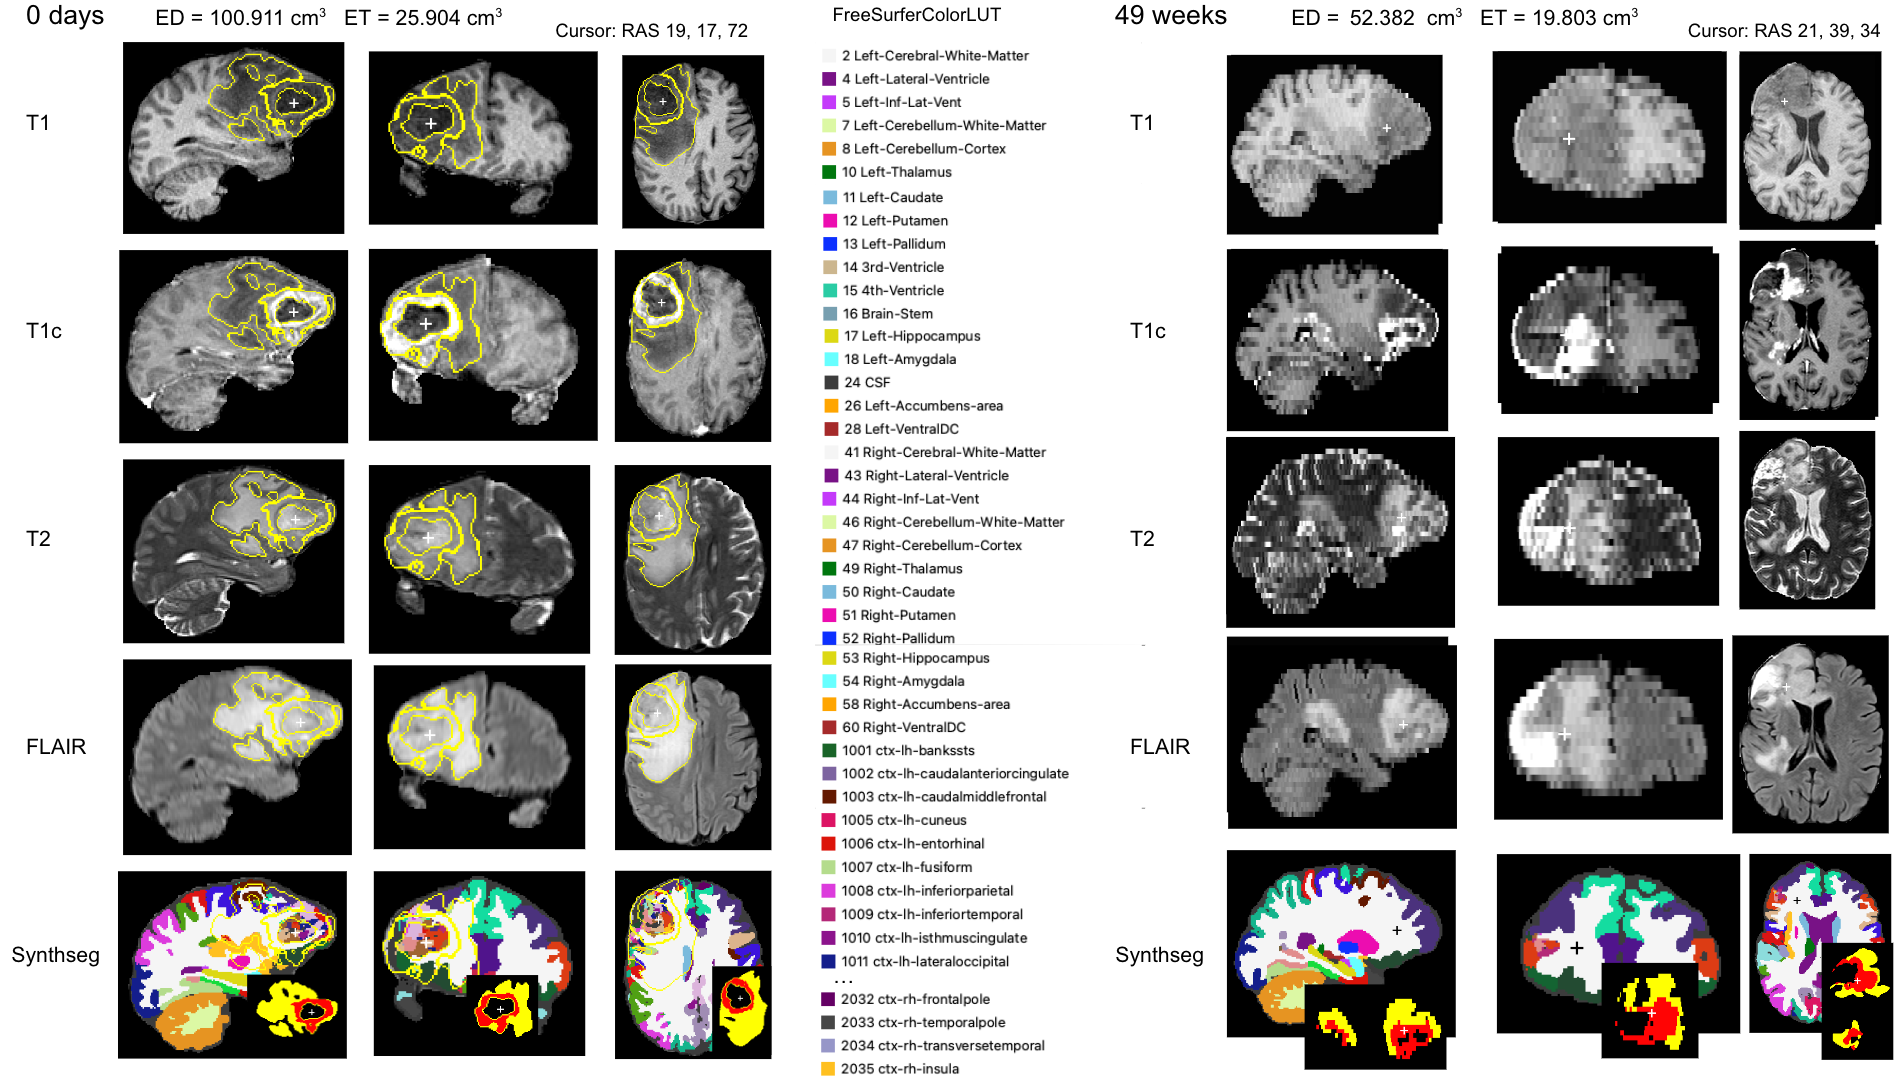
\includegraphics[width=0.99\textwidth]{figs/LUMIERE-Patient-048-hd-glio-synthseg.png}
\end{tabular}
\caption{\textbf{Segmentations of the tumor located in the right frontal lobe and probable underlying anatomical regions in the longitudinal examinations of Patient-048}. For this case the \texttt{FreeSurfer} 7.4.1 \texttt{recon-all-clinical} pipeline was applied to the
T1-weighted acquisitions in in each of the longitudinal examinations of the patient (cf. Figure~\ref{fig:Suter2022_fig2}).
Data from the first visit (day 0) is shown in the left panel,
data from the last visit (week 49) is shown in the right panel.
Visualization of normal and abnormal tissue in the sagittal,
coronal, and axial planes are provided by color-coded overlays using \texttt{Freeview}
and the \texttt{FreeSurferColorLUT} lookup table. The two-compartment tumor segmentations, obtained from HD-GLIO-AUTO, were provided by the LUMIERE team. \emph{Provenance:} the HD-GLIO-AUTO tumor segmentations are courtesy of the LUMIERE consortium~\cite{Suter2022}, and the underlying longitudinal mpMRI examinations are part of the publicly released LUMIERE dataset (\url{https://github.com/ysuter/gbm-data-longitudinal}). The per-subject anatomical overlays in this figure were rendered manually in \texttt{Freeview} on FreeSurfer~7.4.1 \texttt{recon-all-clinical} outputs and provide qualitative context only; the quantitative longitudinal counterpart, computed end-to-end with the unified pipeline (DL segmentation $\cap$ FreeSurfer~8.2.0 \texttt{recon-all-clinical} \texttt{wmparc}), is the longitudinal Hit-Plot of Figure~\ref{fig:lumiere-p048-hitplot-longitudinal}.}
\label{fig:LUMIERE-Patient-048-hd-glio-synthseg}
\end{figure}

\begin{figure}[H]
\centering
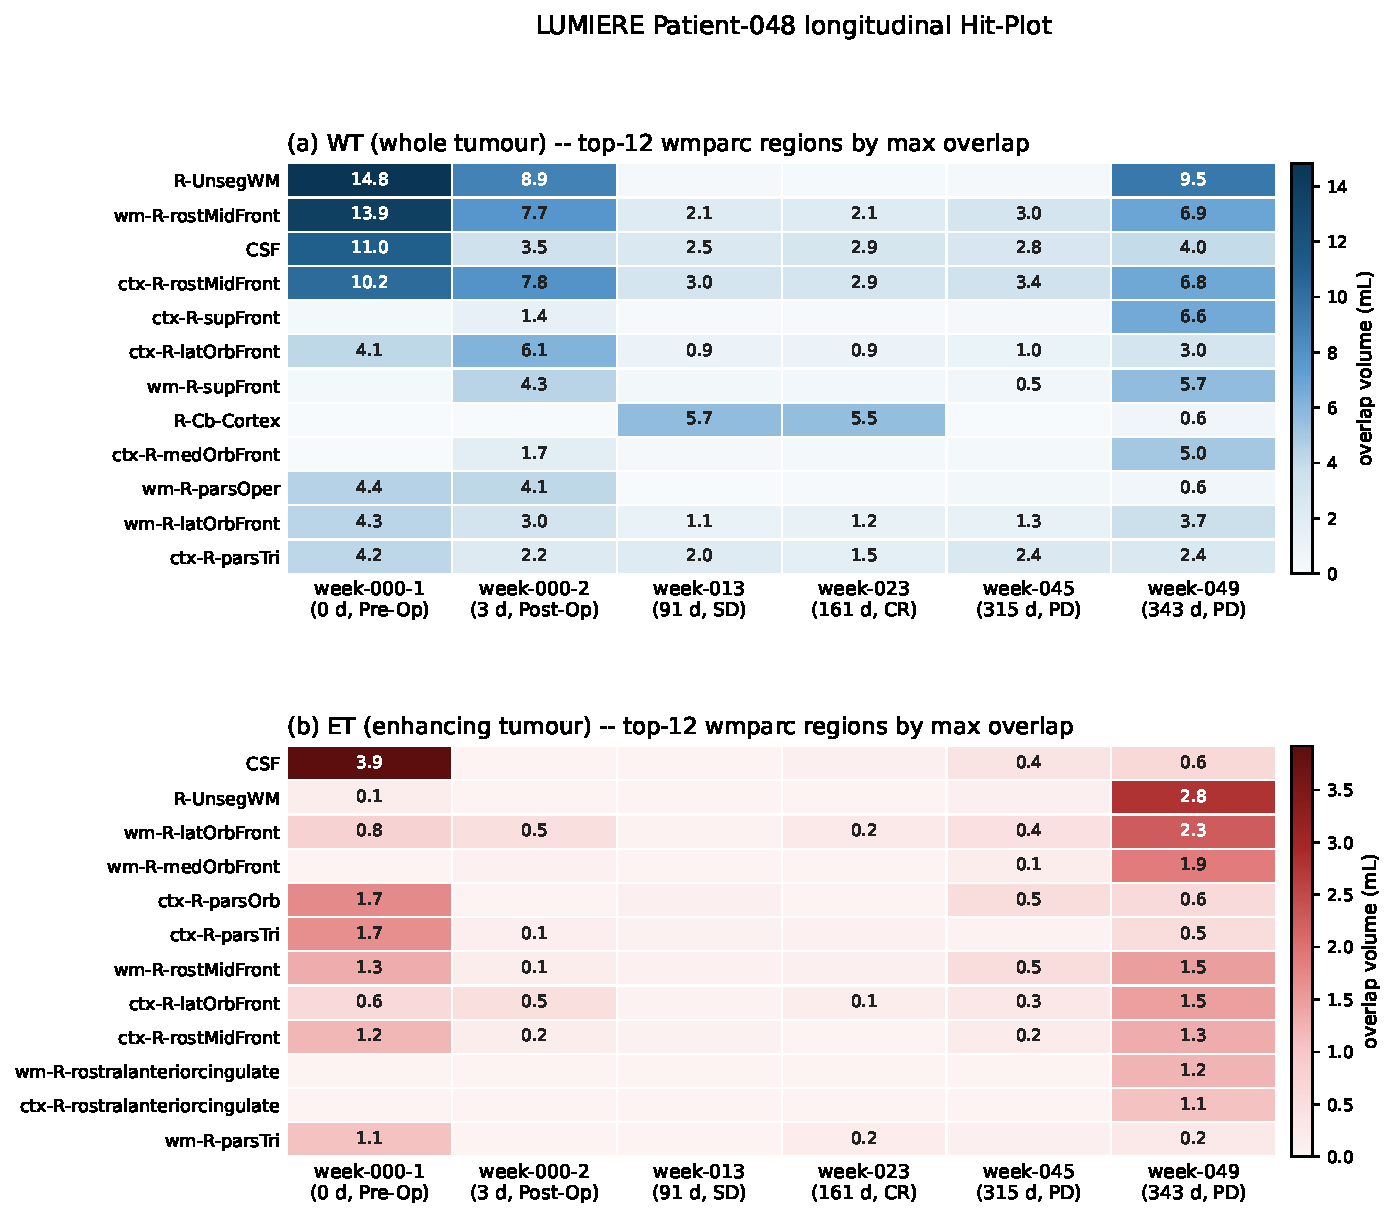
\includegraphics[width=0.70\textwidth]{figs/fig11_lumiere_p048_hitplot.pdf}
\caption{\textbf{LUMIERE Patient-048: longitudinal Hit-Plot across the six examinations.} The anatomy-aware Hit-Plot representation that powers the cohort-level DL-vs-GT agreement panel (Figure~\ref{fig:hitplot-agreement}) is here applied across the Patient-048 longitudinal arc, closing the loop opened by the volume trajectories of Figure~\ref{fig:fig6-lumiere-p048-volumes}: the unified MONAI~Bundle BraTS three-compartment SegResNet (Methods~\S~\emph{Evaluation framework}) is intersected with the FreeSurfer~8.2.0 \texttt{recon-all-clinical} \texttt{wmparc} parcellation on the registered RAS grid of each timepoint. \emph{Top panel} (a) shows the top-12 \texttt{wmparc} regions ranked by maximum WT (whole-tumour) overlap volume across the six visits; cell colour and annotation give the per-cell overlap volume in mL. The Pre-Op (week-000-1, day~0) burden is dominated by right-hemispheric frontal white matter and cortex (\texttt{wm-rh-rostralmiddlefrontal}, \texttt{ctx-rh-rostralmiddlefrontal}, and the FreeSurfer \texttt{Right-UnsegmentedWhiteMatter} catch-all that aggregates tumour-cavity-adjacent white matter), drops sharply at the immediate Post-Op visit (week-000-2, day~3), stabilises through the SD/CR window (week-013, week-023; days~91/161), and recovers in the same anatomical territory at the terminal PD scan (week-049, day~343). \emph{Bottom panel} (b) shows the top-12 \texttt{wmparc} regions for the ET (enhancing-tumour) compartment: the SD and CR visits show near-zero ET across the board (consistent with the radiologically reported clinical CR), and the PD recurrence at week-049 is anatomically colocalised with the original tumour bed, confirming that the right-frontal compartmentalisation is preserved end-to-end through resection $\to$ chemoradiation $\to$ recurrence. The \texttt{Unknown} (FreeSurfer label~0, the catch-all for tumour-cavity\,/\,mass-effect-distorted territory that did not receive a specific anatomical assignment) is omitted from both panels because it carries no anatomical interpretation. \emph{Anonymisation disclosure:} the LUMIERE consortium~\cite{Suter2022} releases visit identifiers as floor-week stamps for re-identification protection; the days-since-baseline labels on the x-axis use the manifest-canonical (0,~3,~91,~161,~315,~343) sequence.}
\label{fig:lumiere-p048-hitplot-longitudinal}
\end{figure}


\vspace{5mm}








\vspace{2mm}


\section{Discussion}


In this feasibility study, we have demonstrated detailed quantitative and automated anatomical profiling
from mpMRI in a leak-safe sample of $n=50$ adult subjects with
IDH-wildtype WHO grade~4 glioblastoma drawn from UCSF-PDGM~v5
(Methods~\S~\emph{Evaluation framework};
Table~\ref{table:ucsf-pdgm-cohort50}), complemented by the LUMIERE
longitudinal subject Patient-048 under the same unified evaluation
framework. This is done to assess macroscopic tumor proliferation
and how the tumor alters and intersects with brain architecture. The pipeline involves
combined 3D segmentation of (i) brain tumor compartments and (ii) the
possible underlying and adjacent brain structures for each tumor
component. A major tool in this profiling was the use of \texttt{SynthSeg}, a
deep learning tool for the segmentation of brain scans of any contrast and
resolution.

Our contribution differs in several ways from the methodological
approach implemented in \texttt{Raidionics} \cite{Bouget2023a}. For the non-local openly available data, the most significant differences
are: (\textbf{i}) We use tumor segmentations that are pre-computed. In case of UCSF-PDGM, the dataset-provided masks (treated as a
per-subject \emph{reference} rather than ground truth, see Methods
~\S~\emph{Evaluation framework} and Limitations item~(vi)), depending jointly on the multiple channels
in the mpMRI recordings (Figures~\ref{fig:UCSF-PDGM-0020-mpMRI} and \ref{fig:Suter2022_fig2}). This provides three biologically different
tumor compartments: ET, NCR, and ED. For the LUMIERE
longitudinal subject (Patient-048) we segment all six examinations
with the unified MONAI~Bundle BraTS three-compartment SegResNet
(Methods~\S~\emph{The LUMIERE dataset};
Figure~\ref{fig:fig6-lumiere-p048-volumes}) and treat the
LUMIERE-team HD-GLIO-AUTO and native CT1-grid DeepBraTumIA masks as
comparators only
(Table~\ref{table:lumiere-p048-comparator-agreement}).
\texttt{Raidionics} computes segmentation of glioblastoma by its pre-trained AGU-Net models.
For preoperative scans it provides a model that produces essentially the same ("BRATS-complient") ET, ED, and NCR compartments as in the UCSF-PDGM dataset.
For postoperative scans, it provides, in the case of GBM, a residual tumor segmentation model that gives a single-valued (one-compartment) mask as output.
(\textbf{ii}) Our pipeline performs direct
segmentation of the native T1 volume without registration to an atlas
template, using the \texttt{recon-all-clinical} pipeline implemented in the
recent version of the open-source \texttt{Freesurfer} software suite. The
pipeline incorporates \texttt{SynthSeg} for segmentation of brain MRI scans of
any contrast and resolution without retraining, and \texttt{SynthSR}, that turn
heterogeneous clinical brain scans into high-resolution T1-weighted
images for 3D morphometry. In effect, these tools provide similar
segmentation results as the \emph{virtual brain grafting} technique by
Radwan and coworkers \cite{Radwan2021}  %
({\small \url{https://github.com/KUL-Radneuron/KUL_VBG}}) enabling whole-brain
parcellation in the presence of large lesions using classical segmentation methods such as the \texttt{recon-all} pipeline in Freesurfer. For obtaining tumor location profiles of cortical and subcortical structures, \texttt{Raidionics} uses (diffeomorphic) imaging registration to a collection of standardized atlases in MNI space, covering cortical and subcortical regions with
different granularity.
This approach typically results in
labeled regions that are only roughly aligned to the patient-specific
sulci and gyri of the cortical sheet, including gray matter, white
matter, and CSF, and only roughly approximating the fine details in
subcortical brain structures of
the underlying and the neighboring anatomy of tumor growth.
(\textbf{iii}) The canonical segmentation engine for all reported
subjects is the MONAI~Bundle BraTS three-compartment SegResNet
(Methods~\S~\emph{Evaluation framework}), with \texttt{segment\_glioma}
and \texttt{Raidionics} as compatible alternatives. The pipeline
enables substitution with any state-of-the-art or new brain tumor
segmentation method
\cite{Alam2021, Bouget2023a, Latif2022, Liu2023, Menze2021, Ranjbarzadeh2022, Thomas2022, Tillmanns2022, WuCao2023}.
The engine runs behind a thin Python adapter that decouples the choice of backbone from
downstream Hit-Plot code.
Per-subject Dice, Hausdorff-95, and volumetric error of the unified
engine against the dataset-provided reference masks are reported in Table~\ref{table:dl-vs-gt}. Hit-Plot-GT versus Hit-Plot-DL agreement is reported per cell as a quantitative measure of the 
Hit-Plot's sensitivity to segmentation variability. A head-to-head
benchmark of the unified engine against \texttt{Raidionics} and
\texttt{segment\_glioma} on the same $n=50$ cohort is methodologically
non-trivial: \texttt{Raidionics} is an atlas-warped pipeline
operating in MNI space whereas HPGS evaluates in native subject
space, so a single-cohort comparison would either resample
\texttt{Raidionics} masks back to native space (and bias
\texttt{Raidionics} downward via interpolation artefacts) or move
HPGS to MNI space (abandoning the native-space architecture argued
for elsewhere in the paper); and the preoperative
\texttt{segment\_glioma} model is trained and deployed on the PICTURE
preprocessing contract (multiparametric MRI rigidly registered to T1c,
N4-corrected, skull-stripped, and affine-registered to SRI-24), whereas
HPGS evaluates on the dataset-provided native co-registered UCSF-PDGM
volumes without re-running that pipeline, so a same-cohort paired
comparison would confound segmenter identity with preprocessing and
operating-space differences rather than isolate backbone quality. We 
leave a methodology-matched comparison to future work. As an
additional bounded sensitivity analysis, we therefore ran
\texttt{mri\_TumorSynth} / nnU-Net~v1.7 on the same $n=50$ staged
mpMRI inputs and report the paired voxel-space metrics
(Table~\ref{table:tumorsynth-agreement}, Figure~\ref{fig:hitplot-agreement-dl-vs-tumorsynth}) and
functional-anatomy Hit-Plot summary (Figure~\ref{fig:functional-anatomy-hitplot-tumorsynth}) in Appendix~5. The TumorSynth
documentation expects skull-stripped inputs registered to the SRI-24
template, whereas this input-matched comparison deliberately uses the
same staged mpMRI inputs as the MONAI~Bundle run. Under these matched-input conditions, Appendix~5 measures the pipeline's sensitivity to the segmentation backbone rather than TumorSynth's best-case accuracy.

A pre-registered outlier audit on the
Table~\ref{table:dl-vs-gt} metrics flagged 16/50 subjects against
the BraTS-2018 strict operating-point band
(WT~$\geq$~0.85, TC~$\geq$~0.75, ET~$\geq$~0.70 Dice; HD95~$>$~20\,mm
on any compartment). Visual adjudication using canonical-RAS
T1c\,/\,reference\,/\,DL panels retained all sixteen: the
dominant flag mode is the MONAI~Bundle's known mild under-segmentation
of the enhancing-tumor boundary (DL\,/\,reference ET-volume ratios in
the 0.55--0.90 range for 15/16 flagged subjects, with WT and TC ratios
mostly in 0.85--1.10), and no flagged case meets a pre-registered
hard-failure rule (lobar miss, contralateral hallucination, or
artefact-dominated mask). Table~\ref{table:dl-vs-gt} is therefore reported over the full $n=50$
cohort with no QC-driven exclusions. The single substantive boundary-disagreement case is documented separately under
Limitations (\S~\emph{Limitations and translational scope}, item~vi).
Using a multicompartment tumor segmentation, as in our case,
facilitates quantitative assessment of the relationship between tumor
enhancement, edema, partial T2-FLAIR mismatch sign, IDH mutational
status, MGMT promoter methylation, and survival in glioblastoma, which
might be of interest in large-scale studies
\cite{Carrillo2012, Lee2023, Pope2005}.\\



\noindent \emph{Strengths and challenges}

\vspace{2mm}

Using the \texttt{SynthSeg} algorithm, producing detailed anatomical parcellations,
covering the whole intracranial 3D space, together with high-quality tumor
segmentation that provides the boundaries of the complex, subject-specific geometry of tumor compartments in 3D, their intersection (\textit{anatomical parcellation} $\cap$ \textit{tumor region})  will have great potential for spatio-temporal
characterization of brain tumor and tumor growth. For each of these
segmented regions and their intersections, the corresponding
spatially restricted multiparametric signal intensity distributions can
be integrated with other methods and software tools, such as
\emph{radiomics} (\cite{Hooper2023}), tumor \emph{growth modeling} (\cite{Mang2020}), or radiation therapy
\emph{planning}.
One challenge for our anatomical profiling features
using mpMRI consisting of (T1, T1c, T2,
FLAIR) only, is that they do not capture information processing neuronal substrate specifically, or the
functional and structural connectivity between different parts of the
brain - the regions and networks that are active during
specific tasks (e.g., perception, motor, speech, working memory,
reasoning). Before resecting a glioblastoma, or in photon or proton therapy, it can be crucial to know
structural connections  and functional areas around the tumor,
especially if it is located near critical regions like those responsible
for language or motor function. Diffusion MRI with fiber-tracking (\cite{Witulla2020}) and
BOLD-fMRI with task-related or resting-state activations (\cite{Nieberlein2023}) can help map
these regions, potentially aiding in preserving them during surgery or radiotherapy.

\vspace{5mm}


\noindent \emph{Future perspectives}

\vspace{2mm}

Building on the recent deep learning approaches to neuro-oncological
imaging, the present methods and case studies introducing anatomical
localization and profiling as shown in this feasibility study, might also influence the evolution
of RANO criteria
\cite{Leao2020, Moon2021, Wen2010, Youssef2023}
for accurate and reproducible radiologic
assessment in patients with glioblastoma.
A possible follow-up of our approach is to more extensively address and evaluate our pipeline to
the large-scale longitudinal LUMIERE dataset,
which is well documented (\cite{Suter2022}) %
and openly available data (on {\small \texttt{figshare.com}})
and code ({\small \url{https://github.com/ysuter/gbm-data-longitudinal}}). On a larger multi-centre grade-4 glioma cohort, our group has recently shown that deep-learning-derived tumour-compartment volumetrics and anatomical tumour trajectories carry independent prognostic information and may inform personalized radiotherapy margin determination \cite{Hannisdal2026}, illustrating the outcome-coupled analyses that the present feasibility pipeline is intended to enable.

There is also accelerated research within \emph{imaging-based
computational oncology} regarding integrating data-driven methods
(machine learning) with model-driven approaches (biophysical priors and
statistical inversion) for predictive modeling of brain tumor growth,
cf. Mang et al. \cite{Mang2020} and the Dagstuhl
Seminar ``Inverse Biophysical Modeling and Machine Learning in
Personalized Oncology" ({\small \url{https://www.dagstuhl.de/23022}}). In this context,
Ezhov and coworkers \cite{Ezhov2023} %
have recently introduced a deep learning-based methodology for inferring
patient-specific spatial distribution of brain tumors from T1-Gd and
FLAIR MRI scans with calibration of their partial differential equation (PDE)
models of glioblastoma growth causing deformation  of
brain tissue ("mass effect").
The growth (forward) models were based on PDEs that describe the evolution of
tumor cell density
in the brain anatomy. The inverse model aims to identify free parameters
of the forward model that best matches the observation, e.g., tumor
outlines from medical imaging and tumor-surrounding tissue types,
anatomical regions, and barriers. In this framework, detailed anatomical mapping of tumor
heterogeneity and tumor environment for use as spatial conditions and
parameter estimates can provide better mathematical modeling of glioma
invasion. Such computational neuro-oncology approaches to personalized
medicine involving spatiotemporal assessment and prediction of brain
tumor growth has opened new avenues of research,
\cite{Alfonso2017,Ezhov2023, Hormuth2022, Lipkova2019, Lipkova2022, Scheufele2019},
where detailed anatomical tumor profiling will be important.

As the field of artificial intelligence increasingly turns its attention
to generative AI and foundation models, neuro-oncological AI is following suit.
In the future, we will likely see
imaging data, their segmentations, anatomical profiling, metadata (tabular), and
the referral information (text) as a single \emph{multimodal document}.
Based on the emergence of multimodal foundation models %
\cite{Moor2023}, this perspective is also expressed within the field of bioimage
analysis \cite{Ma2023, Royer2023}. %
Incorporating image data, free
text descriptions, and quantitative imaging-derived tumor biomarkers into large language models (LLMs) will enable powerful,
case-based Q\&A applications that can be instrumental for
multidisciplinary diagnostics and treatment-planning teams
\cite{Cao2021}  %
and also facilitate patient involvement and understanding.

\vspace{3mm}

A final observation and comment to our anatomical profiling endeavor is related to the highly
influential Brain Tumor Segmentation (\texttt{BraTS}) challenges, which have
focused on the generation of a benchmarking environment and dataset for
the delineation of adult brain gliomas since 2012 \cite{Menze2021, Menze2015}:
\begin{normalsize}
\begin{quote}
\emph{\ldots{} For brain tumor patients, the image acquisition time
series typically starts with an already pathological scan. This poses
problems, as many algorithms are designed to analyze healthy brains and
provide no guarantees for images featuring lesions. Examples include but
are not limited to algorithms for brain anatomy parcellation, tissue
segmentation, and brain extraction. To solve this dilemma, we introduce
the BraTS inpainting challenge \ldots{}}
\end{quote}
\end{normalsize}

These statements further indicate the importance and relevance of our
contribution in the direction of computational oncology and precision
imaging.

\subsection*{Limitations and translational scope}

The present study is a feasibility and infrastructure report: it
establishes a reproducible, native-space anatomy-profiling pipeline and
quantifies its segmentation and Hit-Plot behaviour, but it does not test
clinical utility. We therefore explicitly delimit the claims it can
support. (i)~\textbf{Cohort and generalisability.} The
evaluation cohort is n=50 GBM
(IDH-wildtype, WHO grade~4) subjects from a single public dataset
(UCSF-PDGM~v5, Sex $\times$ OS-tertile stratified, leak-safe with respect
to BraTS21 Training, see Methods § \emph{The UCSF-PDGM dataset} and
Table~\ref{table:ucsf-pdgm-cohort50}). Although the cohort is sufficient
to characterise the pipeline's per-compartment segmentation and
parcellation behaviour, multi-centre, prospective, treatment-stratified
data (ideally including paired baseline / post-operative / follow-up
exams from independent institutions) will be required before any
generalisability statement to routine neuro-oncology practice can be
made.

(ii)~\textbf{Radiotherapy claims.} The
phrase ``sculpt dose distributions'' (Introduction, in reference to
modern IMRT/VMAT delivery~\cite{Niyazi2023,Palma2019}) describes the capability of
the radiotherapy delivery technology, not of our pipeline. Our pipeline
contributes a more detailed, subject-specific anatomical substrate over
which a treatment planner could in principle reason. It does not itself generate, modify, or validate dose distributions, and we have not
performed any dosimetric or treatment-planning evaluation in this work.
A prospective evaluation against a dosimetric end-point (e.g.\ NTCP for
a defined organ-at-risk such as the contralateral hippocampus) is the
appropriate next step and is outside the scope of the present
manuscript.

(iii)~\textbf{Margin-reduction claims.}
The ESTRO--EANO 2023 reduction of the post-operative CTV margin from
20\,mm to 15\,mm cited in the Introduction is a clinical
guideline change reported by Niyazi et~al.~\cite{Niyazi2023}. We do not claim that our pipeline justifies, enables,
or quantifies a further reduction of the CTV/PTV margin in any patient.
Investigating whether anatomy-aware target-volume editing (e.g.\
restricting CTV expansion at known anatomical barriers identified by
\texttt{recon-all-clinical} parcellations) can be performed safely will
require a dedicated planning study with explicit recurrence-pattern
analysis.

(iv)~\textbf{Translational and outcome claims.} We do not report any patient-outcome end-point (overall
survival, progression-free survival, neurocognitive performance,
quality-of-life). The Hit-Plot / regional-tumour-burden representation
is descriptive and is presented as an exploratory anatomical profile
suitable for hypothesis generation, not as a clinically actionable
biomarker. This applies equally to the functional-anatomy appendix
summary and its OS-tertile small multiples: they show readability and
metadata stratification of the same Hit-Plot quantities, not an
association between regional burden and survival. Statements in the
Introduction and Discussion concerning
``preserving cognitive function'' or ``new therapeutic strategies'' refer
to the broader literature on tumour--neuron interactions
(e.g.~\cite{Krishna2023, Ibrahim2023}) and are not conclusions of this
study. A formal translational claim would require: (a)~prospective,
multi-centre validation of the segmentation and parcellation against
expert manual reference for each compartment with standardised metrics
(Dice, HD95, volumetric error, sensitivity, specificity; reported in Table~\ref{table:dl-vs-gt} for our evaluation cohort); (b)~a planning- or
outcome-coupled study with predefined end-points; and (c)~a regulatory
pathway appropriate for the intended clinical use.

(iv-bis)~\textbf{Hit-Plot-to-outcome as a named follow-up.}
The UCSF-PDGM metadata summarised in
Table~\ref{table:ucsf-pdgm-cohort50} include overall survival, OS
tertile, MGMT promoter status, and extent of resection for all
$n=50$ subjects of the evaluation cohort. A natural follow-up
question is whether the per-subject Hit-Plot, or a low-dimensional
summary of it (hemispheric asymmetry, lobar burden, or
functional-anatomy group burden, optionally stratified by
compartment), carries prognostic information beyond known clinical
covariates (age, EOR, MGMT, treatment intensity). We deliberately do not
perform that analysis in the present feasibility report. Under the
same metadata filters used here (GBM, IDH-wildtype, WHO grade~4;
known OS; no biopsy before imaging; exclusion of BraTS21 Training
subjects), the UCSF-PDGM metadata support an expanded leak-safe pool
of approximately 110 baseline subjects, with roughly balanced OS
tertiles and a larger event count. That pool is a sensible next
dataset for a pre-specified, low-dimensional regional-burden analysis,
but using it would require re-running the segmentation, parcellation,
Hit-Plot, QC, and manuscript-generation chain and is therefore a possible
dedicated follow-up study. An honest test would require: a pre-registered design with
dimensionality reduction applied before any per-region claim; a
regularised Cox proportional-hazards model with age, EOR, MGMT, and
treatment-intensity covariates forced in; FDR control over the
remaining anatomical predictors; internal cross-validation; and
external validation on an independent multi-centre cohort
(e.g.\ BraTS21 Survival, UPenn-GBM, or a prospective
multi-institutional set). At $n=50$ subjects with $\sim$300
candidate (region, compartment) features and $\sim$30 observed
events, the present cohort is statistically underpowered for a
primary survival analysis, and even the larger UCSF-PDGM-only
derivation pool would not by itself support a generalisability claim.
The \emph{Hit-Plot-to-outcome} variant is
the natural follow-up this analysis points to.

(v)~\textbf{Methodological scope.} The pipeline is built from
established open-source components (the MONAI~Bundle BraTS
three-compartment SegResNet for tumor segmentation, the unified
engine of Methods §~\emph{Evaluation framework}; FreeSurfer 8.2.0
\texttt{recon-all-clinical} for anatomical parcellation, with
SynthSeg and SynthSR as its contrast-/resolution-agnostic core
models; HD-BET for skull stripping; HD-GLIO-AUTO and DeepBraTumIA
retained as comparators against the unified engine on the LUMIERE
longitudinal subject,
Table~\ref{table:lumiere-p048-comparator-agreement}). The contribution of this work lies in the integration, the
anatomy-aware Hit-Plot representation, and the reproducible
end-to-end orchestration. The same unified engine plus
FreeSurfer~8.2.0 \texttt{recon-all-clinical} \texttt{wmparc}
pipeline drives both the cohort-level DL-vs-GT Hit-Plot agreement
panel for the $n=50$ UCSF-PDGM cohort
(Figure~\ref{fig:hitplot-agreement}) and the longitudinal
Patient-048 Hit-Plot
(Figure~\ref{fig:lumiere-p048-hitplot-longitudinal}), so the same
parcellation-$\cap$-segmentation framework is exercised end-to-end
on both the leak-safe cross-sectional cohort and the longitudinal
arc without methodological substitution. Discriminating the
relative contribution of each component to downstream features will
require ablation studies. A
methodology-matched head-to-head benchmark of the unified engine
against \texttt{Raidionics} and \texttt{segment\_glioma} (i.e.\ on
a cohort, modality set, and spatial frame of reference where each
comparator is on its own methodological home ground) is another
standing future-work item.

(vi)~\textbf{Reference-mask quality and cross-segmenter
disagreement.} The UCSF-PDGM tumor masks used as reference for the
$n=50$ segmentation evaluation (Table~\ref{table:dl-vs-gt}) are themselves the output of a
specific human-plus-algorithmic annotation protocol and are
treated as a \emph{reference} rather than ground truth. The
pre-registered outlier audit reported in Methods (\S~\emph{Per-subject
outlier audit on Table~\ref{table:dl-vs-gt}}) identifies one subject (sub-0396) as a
worst-case exemplar of cross-segmenter boundary disagreement: the
unified MONAI~Bundle pipeline labels a confluent necrotic-core +
enhancing-rim region (${\sim}17$\,cc) within the central lesion,
whereas the dataset-provided reference labels the same region
predominantly as edema (reference TC ${\sim}2$\,cc on a ${\sim}88$\,cc
total lesion). Without expert clinical adjudication beyond the scope
of this study, we cannot determine which segmentation is closer to
the underlying tumour biology. The case is rendered as a standalone
T1c\,/\,reference\,/\,DL panel in the supplementary material
(produced by the same canonical-RAS pipeline used for Figure~2),
and sub-0396 is retained in
Table~\ref{table:dl-vs-gt} to keep the reported distribution faithful
to the true cross-segmenter behaviour on this cohort.

(vii)~\textbf{Per-region sunbursts and functional-anatomy label
groups.} Per-region anatomical-profile sunbursts at single-subject
and cohort-stratified levels are descriptive at $n{=}1$ and aggregate
poorly when collapsed to coarse anatomical lobes (which discards the
per-region resolution that the rest of the Hit-Plot variants are
designed to expose). The cohort-level lobe distribution is therefore
reported as a quantitative prose statement in
Methods~\S~\emph{The UCSF-PDGM dataset} rather than as a sunburst.
The compact functional-anatomy summary in Appendix~4 is a more
readable aggregation, and is included because it fits as one
descriptive figure plus one cautious Results paragraph. Appendix~5 repeats the same aggregation after swapping the segmentation backbone
to \texttt{mri\_TumorSynth} / nnU-Net~v1.7 as a bounded sensitivity
check. Both appendices remain
anatomical-label adjacency analyses derived from \texttt{wmparc}: the
motor-adjacent, left-language-adjacent, and deep-midline /
commissural groups are not tractography, individualized eloquence
mapping, fMRI, organ-at-risk proximity, treatment-planning validation,
or outcome prediction.
Proper per-region sunbursts, tract / organ-at-risk proximity
profiles, and Hit-Plot-to-outcome models are deferred to follow-up
studies where cohort size, clinical annotations, and independent
validation can support those stronger claims.

\section{Code and data availability}
\begin{sloppypar}
The UCSF-PDGM dataset used in this study is publicly available from
The Cancer Imaging Archive (TCIA)
(\url{https://doi.org/10.7937/tcia.bdgf-8v37}). The LUMIERE dataset
is publicly available at
\url{https://github.com/ysuter/gbm-data-longitudinal}. All
processing code, the pinned software stack, the cohort-pinning
manifests for the $n=50$ UCSF-PDGM evaluation cohort and for the
six-timepoint LUMIERE Patient-048 longitudinal subject, and the
producer scripts that generate every figure and table reported
above end-to-end from the on-disk derivatives will be released at
\url{https://github.com/arvidl/high-precision-glioma-segmentation}.
The qualitative LUMIERE Patient-048 panel of
Figure~\ref{fig:LUMIERE-Patient-048-hd-glio-synthseg} was produced
manually in \texttt{Freeview} on FreeSurfer~7.4.1
\texttt{recon-all-clinical} outputs. The panel-composition recipe is available from the corresponding author on request.
\end{sloppypar}

\section*{Author contributions}
Conceptualization: A.L.\ and S.A.; methodology: A.L., A.S.L., and S.A.; software: A.L., A.S.L., and S.A.; validation: A.L.\ and S.A.; formal analysis: A.L.\ and A.S.L.; investigation: A.L., A.S.L., S.A., and M.H.H.; resources: A.L., A.S.L., and M.C.; data curation: A.L.; writing, original draft: A.L.; writing, review and editing: A.L., A.S.L., S.A., D.G., M.H.H., and M.C.; visualization: A.L.\ and S.A.; supervision: A.L., A.S.L., and M.C.; project administration: A.L.; funding acquisition: A.L., A.S.L., and M.C. All authors reviewed the manuscript and agreed to its submission.

\section*{Funding}
This work was supported by the Trond Mohn Research Foundation under Grant BFS2018TMT07; the Norwegian Cancer Society (Kreftforeningen) under Grant 190170; and the National Programme for Clinical Treatment Research in the Specialist Health Services (KLINBEFORSK).

\section*{Institutional review board statement}
The study was conducted in accordance with the Declaration of Helsinki. For the UCSF-PDGM dataset, imaging studies were approved by the University of California, San Francisco institutional review board with a waiver of informed consent, as described in the original dataset publication~\cite{Calabrese2022b}. The LUMIERE dataset was collected under institutional review board approval at the University Hospital of Bern, Switzerland~\cite{Suter2022}. No additional ethical approval was required for the re-analysis of these publicly available, anonymised datasets.

\section*{Declaration of generative AI use}
During preparation of this manuscript, the authors used Cursor (version 3.x) with the Composer~2.5 agent to assist with pipeline software development and language editing of the text. The tool was used to accelerate implementation and revision of analysis code and to improve clarity of the prose. It was not used to generate scientific results, figures, or reference lists without human verification. The authors reviewed and edited all AI-assisted output and take full responsibility for the content of the published article.

\setstretch{1.0}  %


\section*{Abbreviations}
The following abbreviations are used in this manuscript:\\

\noindent
\begin{tabular}{@{}ll}
ANTs & Advanced Normalization Tools (software toolkit) \\
ART & Adaptive radiotherapy planning \\
ASL & Arterial spin labeling (pMRI measurement technique) \\
BOLD & Blood oxygenation level-dependent (fMRI measurement technique)\\
BraTS & Brain Tumor Segmentation (challenges) \\
CCC & Concordance correlation coefficient \\
CSF & Cerebrospinal fluid \\
CTV & Clinical target volume \\
DCE-MRI & Dynamic susceptibility contrast MRI with the administration of a contrast agent \\
DR & Domain randomization \\
dMRI & Diffusion MRI \\
eTIV & Estimated total intracranial volume \\
fMRI & Functional MRI \\
ED  & Tumor region with edema \\
EOR & Extent of resection \\
ESTRO & European Society for Radiotherapy \& Oncology \\
ET & Enhancing tumor region \\
FA & Fractional anisotropy \\
FLAIR & Fluid attenuated inversion recovery (MRI measurement technique)\\
GBM & Glioblastoma\\
GSI-RADS & Glioblastoma Surgery Imaging Reporting And Data System \\
GTR & Gross total resection \\
GTV & Gross tumor volume \\
HARDI & High-angular-resolution diffusion imaging (MRI measurement technique) \\
HD$_{95}$ & 95th-percentile Hausdorff distance \\
HGG & High-grade glioma \\
ICV & Intracranial volume \\
IDH & Isocitrate dehydrogenase (enzyme)\\
IMRT &  Intensity-modulated radiotherapy \\
MGMT & O6-methylguanine-DNA methyltransferase (enzyme) \\
MNI & Montreal Neurological Institute \\
mpMRI & Multiparametric MRI \\
NCR & Necrotic tumor region \\
NET & Non-enhancing tumor region \\
NTCP & Normal tissue complication probability (models) \\
OAR & Organs at risk \\
OS & Overall survival \\
PCR & Polymerase Chain Reaction \\
PTV & Planning tumor volume \\
RANO & Response Assessment in Neuro-oncology (criteria) \\
scRNA-seq &  Single-cell RNA sequencing \\
STR & Subtotal resection \\
SWI & Susceptibility-weighted imaging (MRI measurement technique) \\
SyN & Symmetric normalization: Affine + deformable transformation \\
pMRI & Perfusion MRI \\
RT  & Radiotherapy \\
TC & Tumor core \\
TCGA & The Cancer Genome Atlas \\
TCIA & The Cancer Imaging Archive \\
TME & Tumor microenvironment\\
UCSF-PDGM & University of California San Francisco Preoperative Diffuse Glioma (dataset)\\
WT & Whole tumor or Wild type
\end{tabular}

\section*{Acknowledgements}
The UCSF-PDGM dataset was produced with data obtained under NIH Ruth L. Kirschstein Institutional National Research Service Award grants NCI U01CA242871 and T32EB001631, and RSNA Research \& Education Foundation grant RR2011.

\section*{Disclosure statement}
The authors report there are no competing interests to declare.

\newpage


\bibliography{references}


\bibliographystyle{abbrv}


\newpage


\section*{\large APPENDIX 1. Examples of image data from the UCSF-PDGM and LUMIERE datasets}

\vspace{15mm}

\subsection*{UCSF-PDGM}

\begin{figure}[H]
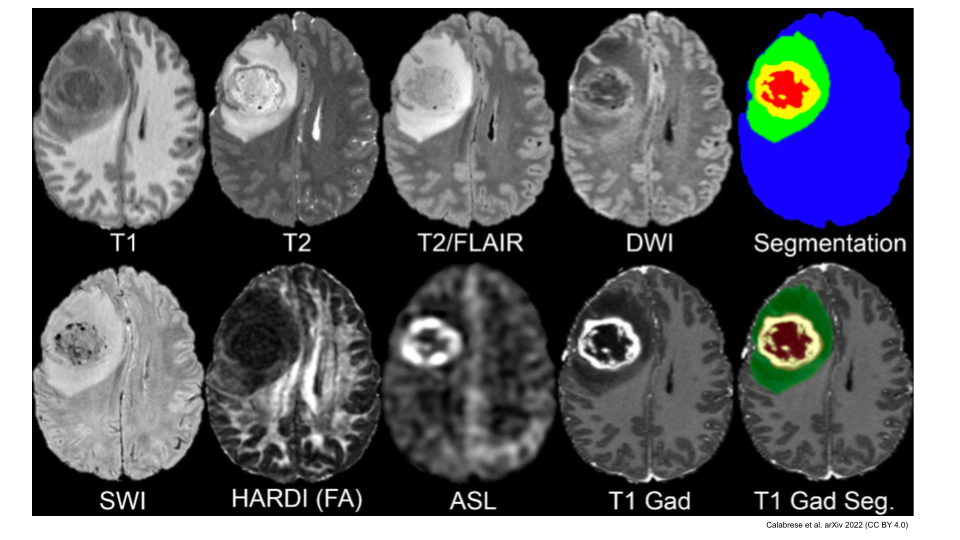
\includegraphics[width=0.99\textwidth]{figs/glioma-localization-figs-calabrese-2022.png}
\caption{\textbf{Example of multiparametric MRI examination in a 37-year-old man from the UCSF-PDGM dataset}. The original recordings have been subject to non-linear co-registration, resampling, and skull stripping.  T1: T1-weighted pre-contrast, T2: T2-weighted, T2/FLAIR: T2-weighted FLAIR, DWI: isotropic (trace) diffusion-weighted image, SWI: susceptibility-weighted image, HARDI (FA): fractional anisotropy derived from high-angular-resolution diffusion imaging (HARDI) data, ASL: arterial spin labeling perfusion, T1 Gad: T1-weighted post-contrast, Segmentation: multicompartment tumor segmentation (blue = brain, green = FLAIR abnormality, yellow = enhancing tumor, red = necrotic core), T1 Gad Seg.: tumor segmentation semitransparent overlay on T1-weighted post-contrast image. We used the mpMRI subset \{T1, T1 Gad, T2, T2/FLAIR, Segmentation\} for the present study.\\ From Calabrese et~al.~\cite{Calabrese2022b} {\small \url{https://arxiv.org/abs/2109.00356}} (CC BY 4.0).}
\label{fig:UCSF-PDGM-Calabrese-2022}
\end{figure}

\begin{figure}[H]
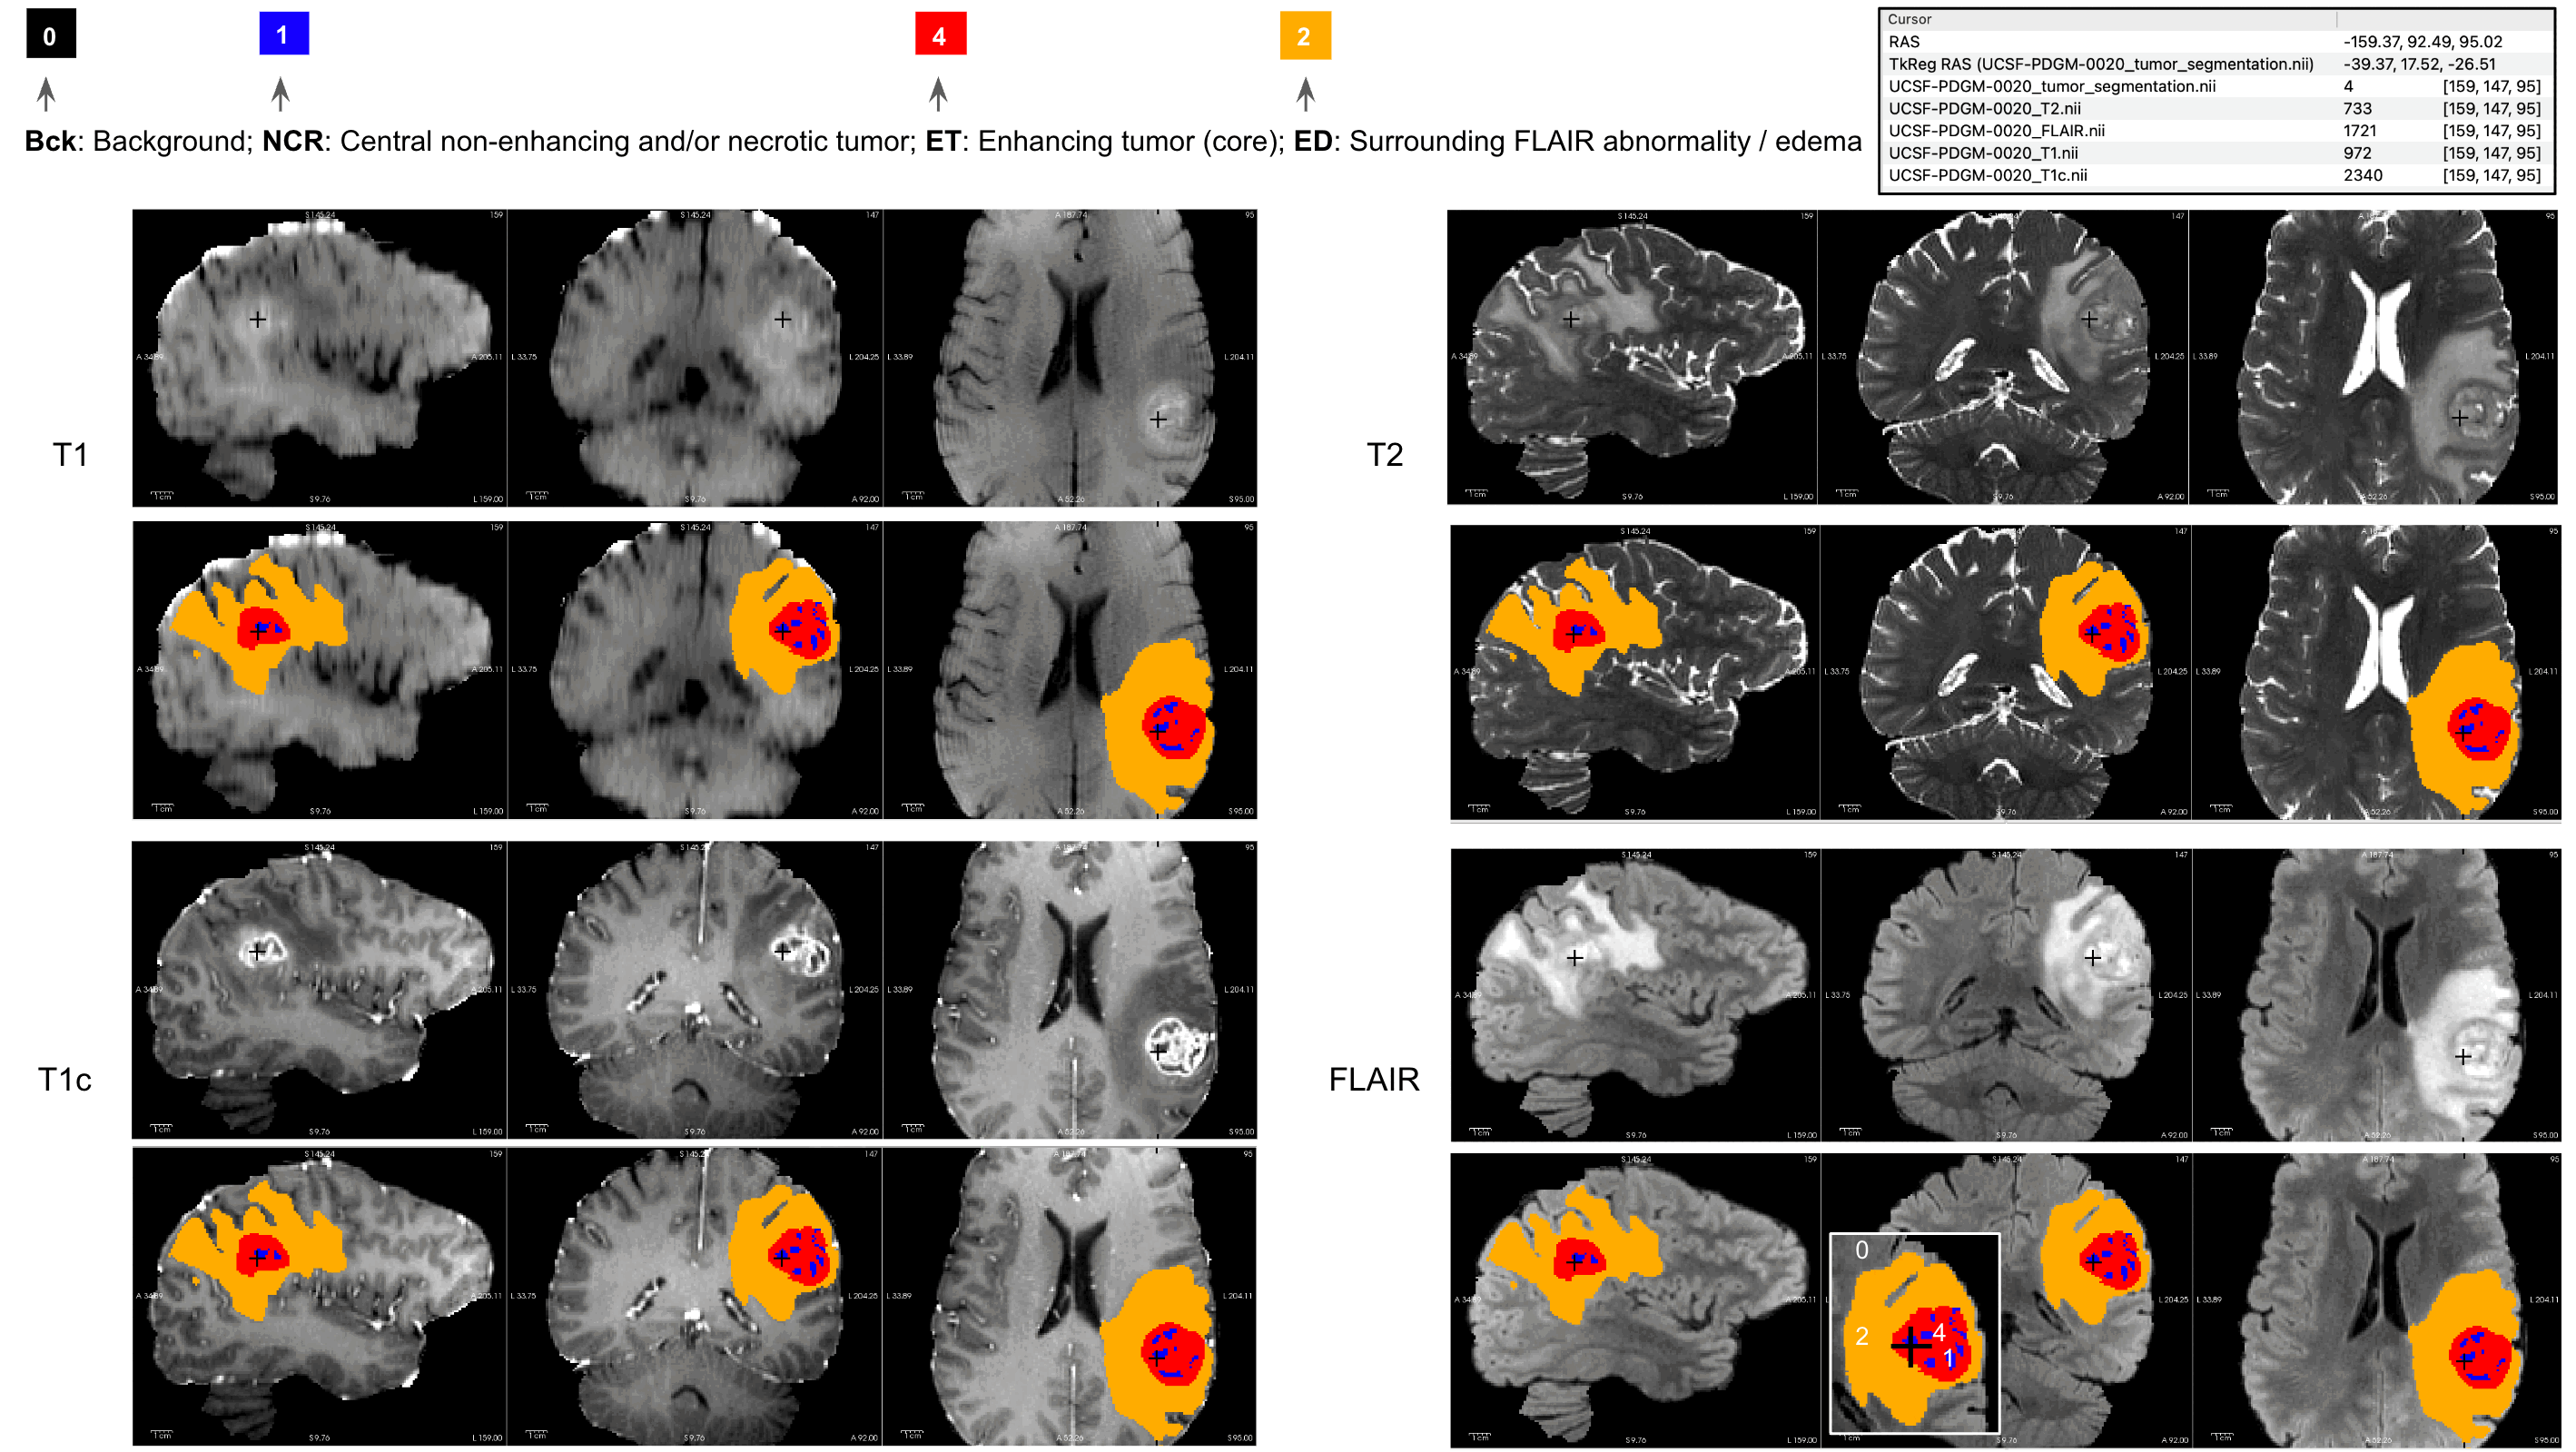
\includegraphics[width=0.98\textwidth]{figs/glioma-localization-figs-UCSF-PDGM-0020-mpMRI.png}
\caption{\textbf{Illustration of the mpMRI data and tumor segmentation using the UCSF-PDGM-0020 examination}. Each of the four channels (T1, T1c, T2, and FLAIR) is shown separately as rows in the panels, with the corresponding color-coded three-compartment tumor segmentation mask as an overlay, shown below. A sagittal, a coronal, and an axial slice are the columns in the panels. The center of the black crosshair is fixed at coordinates [\texttt{i=159}, \texttt{j=147}, \texttt{k=95}] in all panels, using the interactive \texttt{Freeview} tool. The mapping of tumor component labels (NCR, ED, ET) to integer values (1, 2, 4) and color-codes is shown in the upper panel.}
\label{fig:UCSF-PDGM-0020-mpMRI}
\end{figure}

\subsection*{LUMIERE}


\begin{figure}[H]
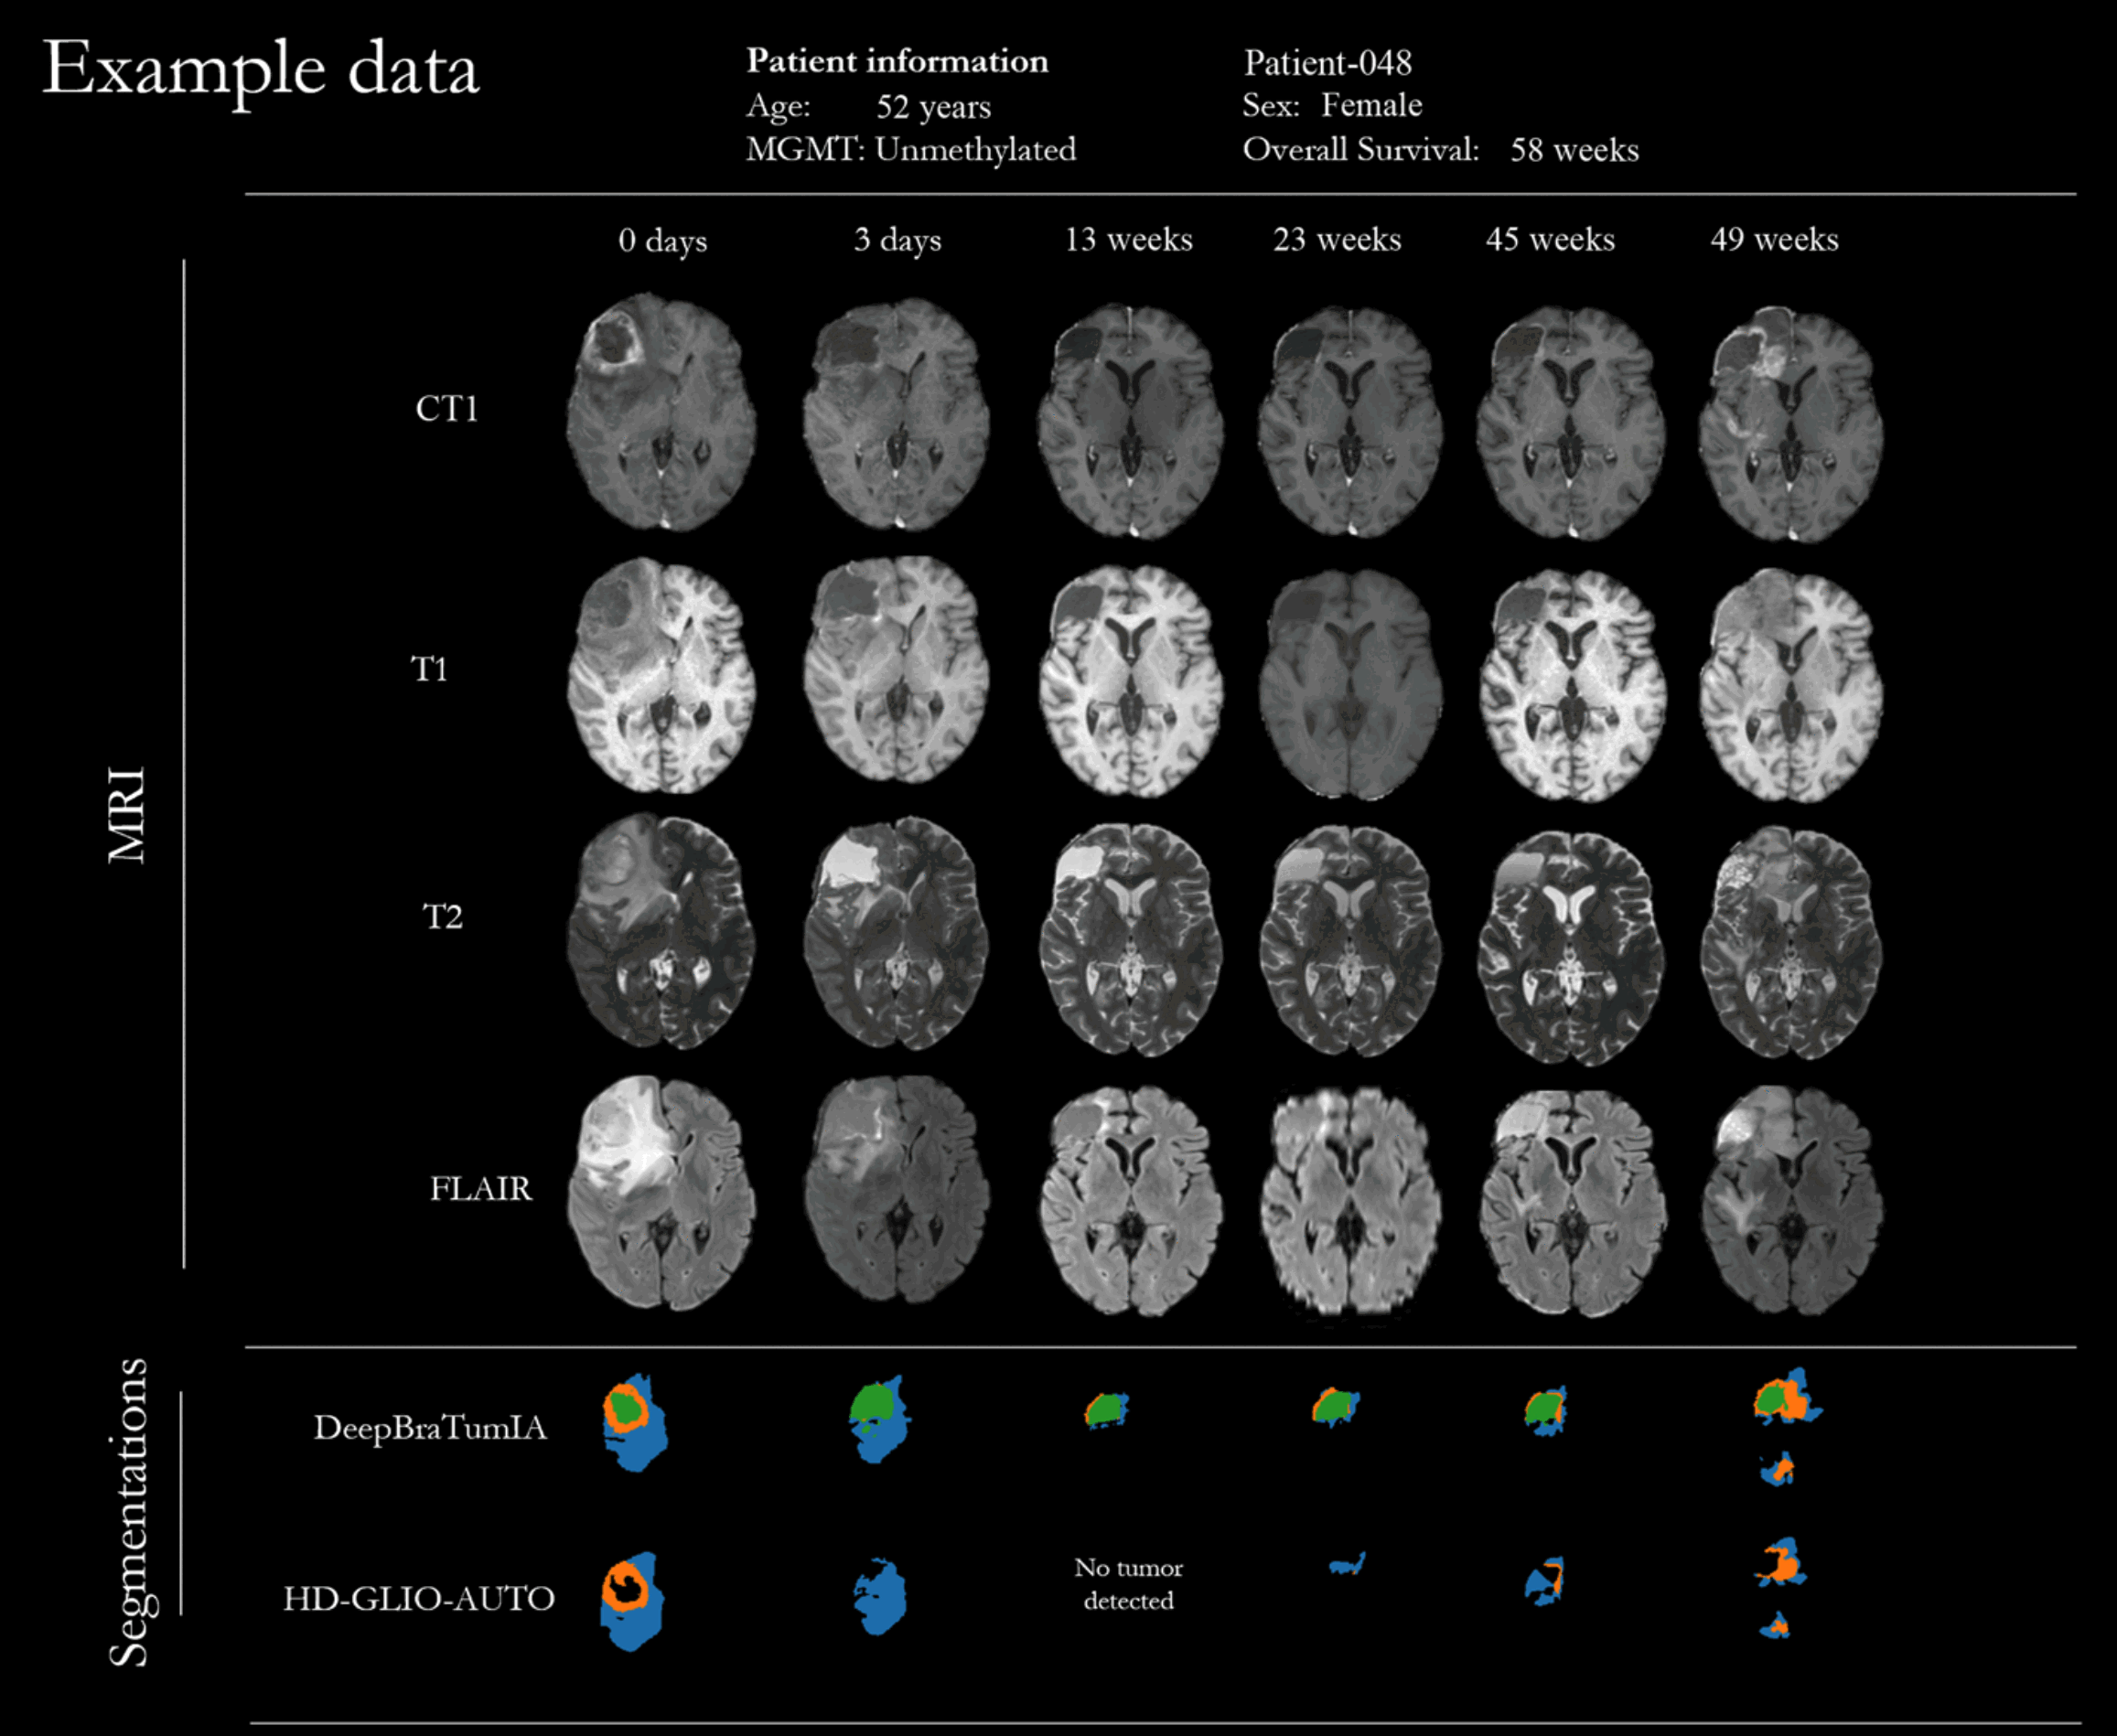
\includegraphics[width=0.99\textwidth]{figs/Suter2022_fig2.png}
\caption{\textbf{Example of longitudinal data on GBM from the LUMIERE collection}. CT1/T1: Post-/pre-contrast T1-weighted, T2-weighted, and fluid-attenuated inversion recovery (FLAIR). For this individual, the entire contrast enhancement was fully removed. Following a phase of complete response, there was a progression characterized by a highly rapid growth rate. In the present study we process all six mpMRI examinations of Patient-048 under the unified evaluation framework (Results, Figure~\ref{fig:fig6-lumiere-p048-volumes}). \\ From Suter et al. \cite{Suter2022} {\small \url{https://www.nature.com/articles/s41597-022-01881-7} (CC BY 4.0)}.}
\label{fig:Suter2022_fig2}
\end{figure}


\section*{\large APPENDIX 2. Anatomical profiling results from cases UCSF-PDGM-0039, -0066, and -0085}



\begin{figure}[H]
\begin{tabular}{c}
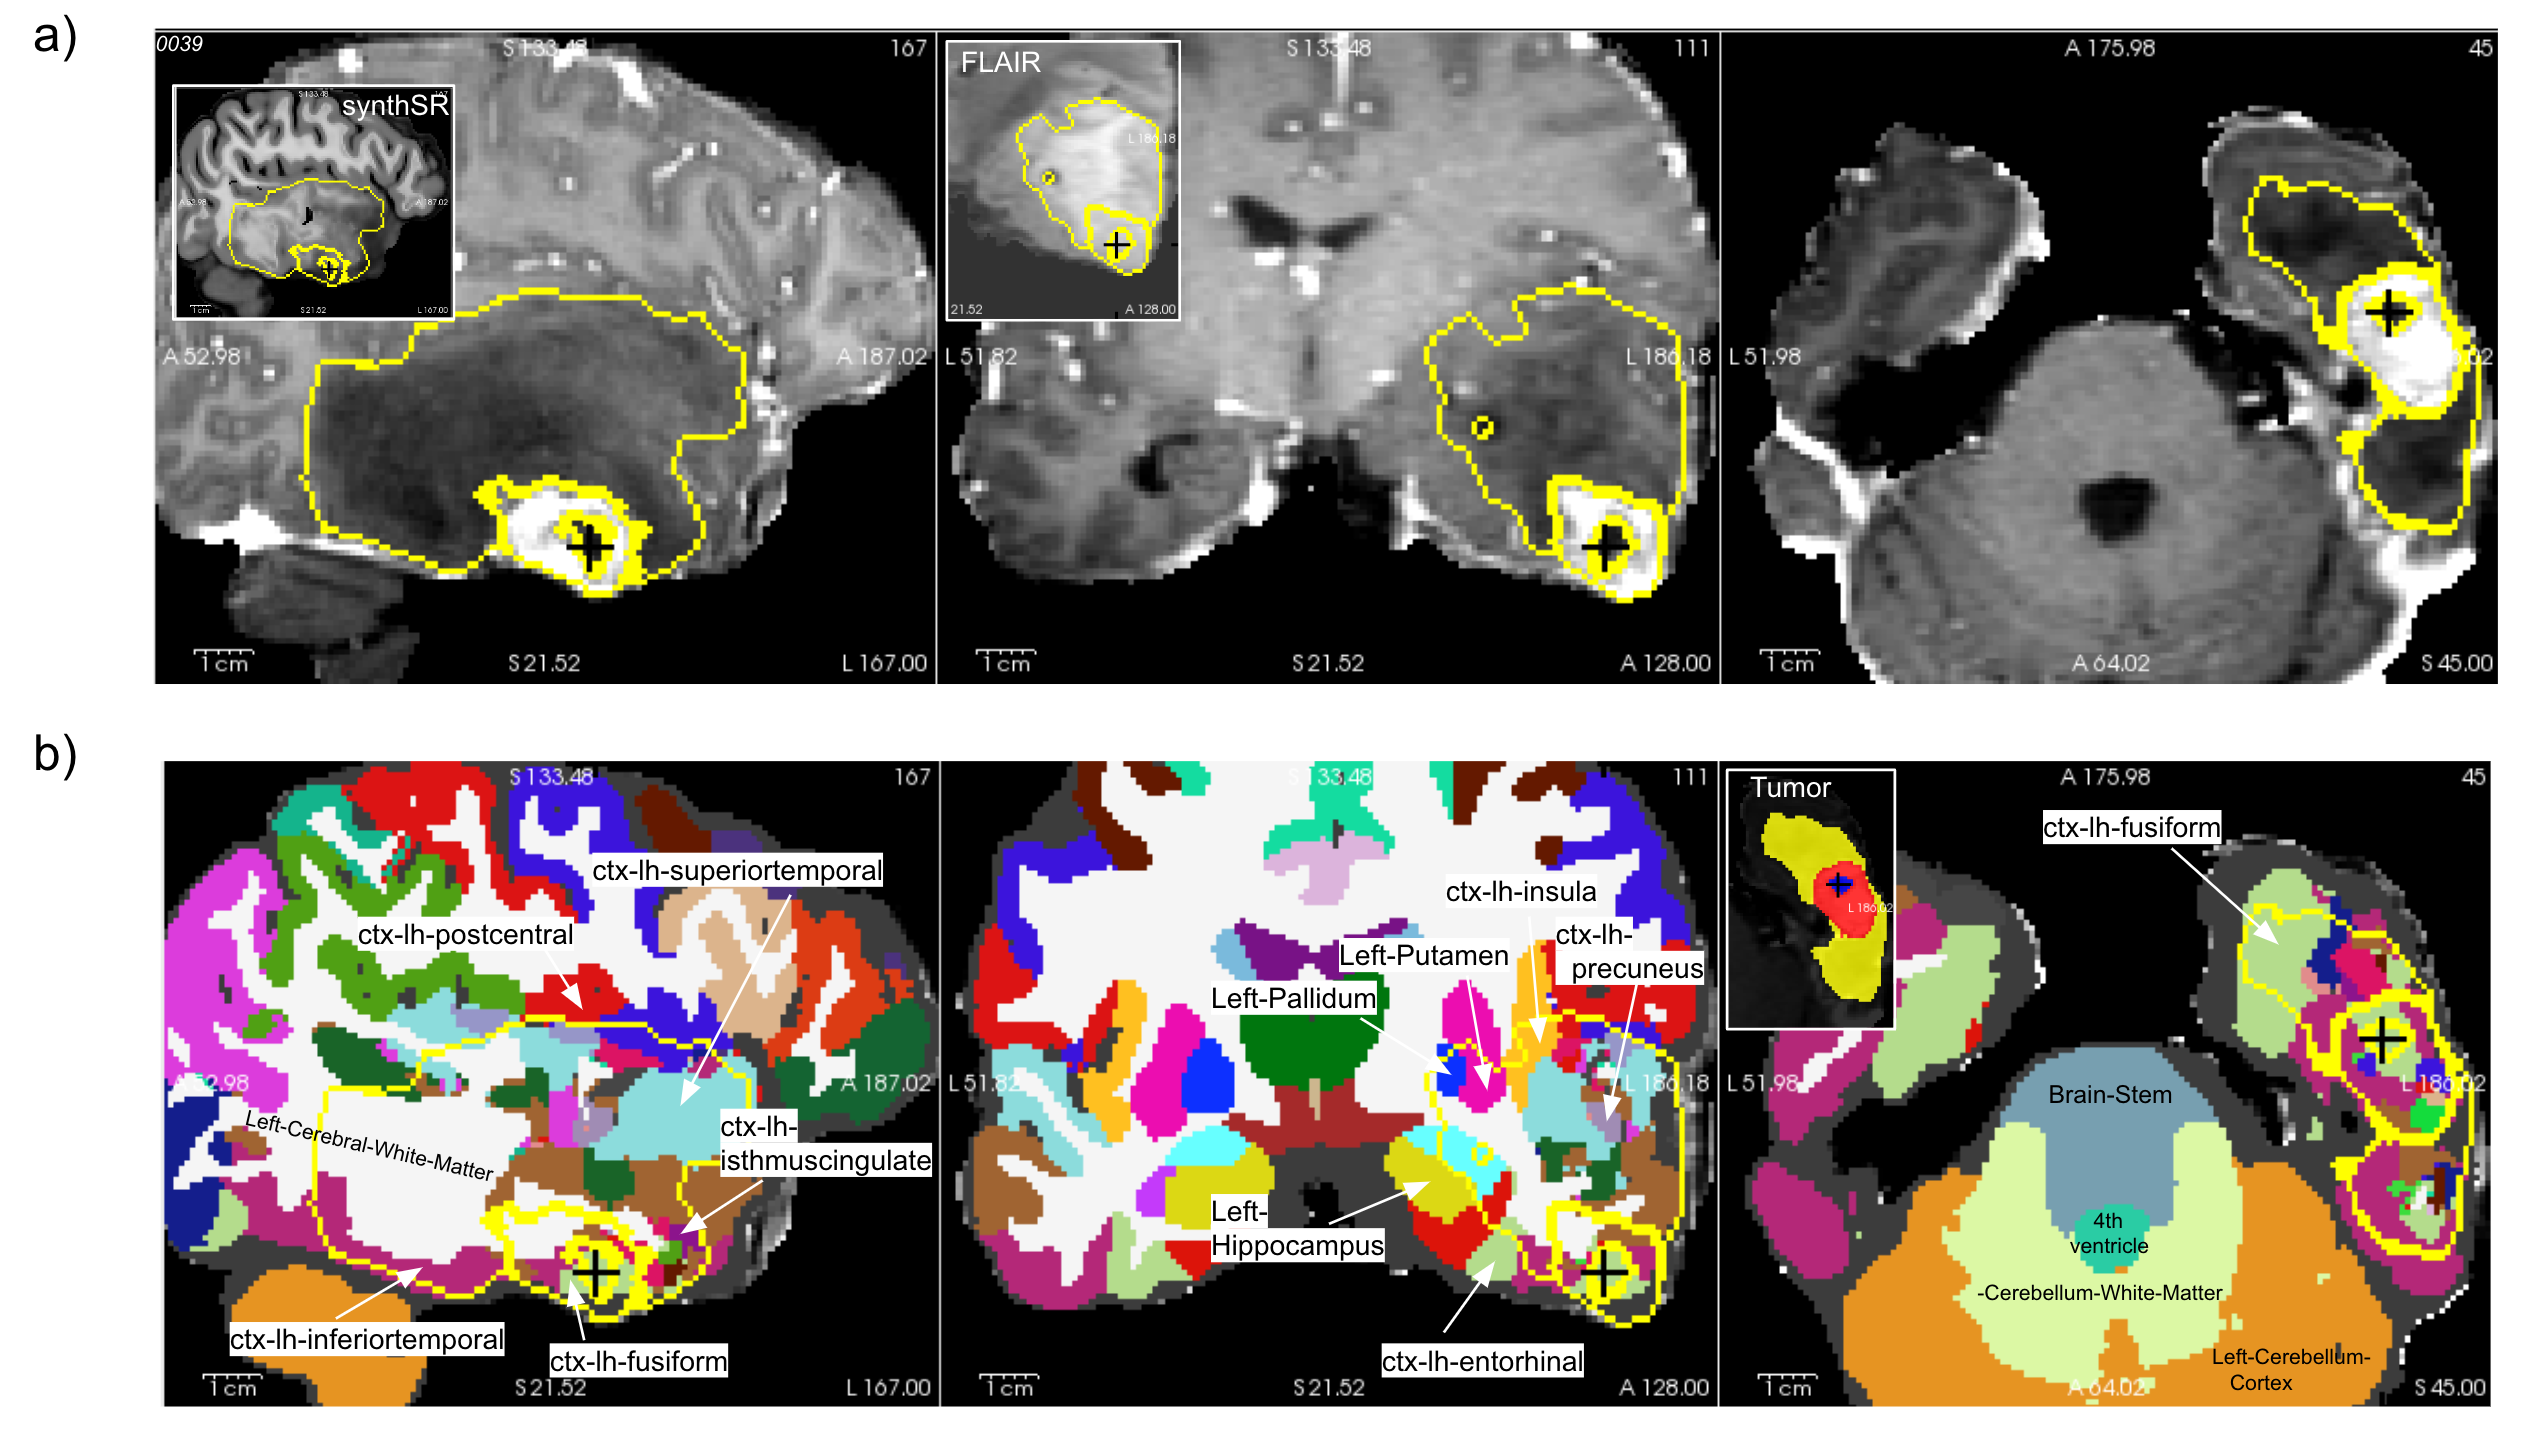
\includegraphics[width=0.98\textwidth]{figs/glioma-localization-figs-UCSF-PDGM-0039-tumor-contours-on-synthseg.png} \\
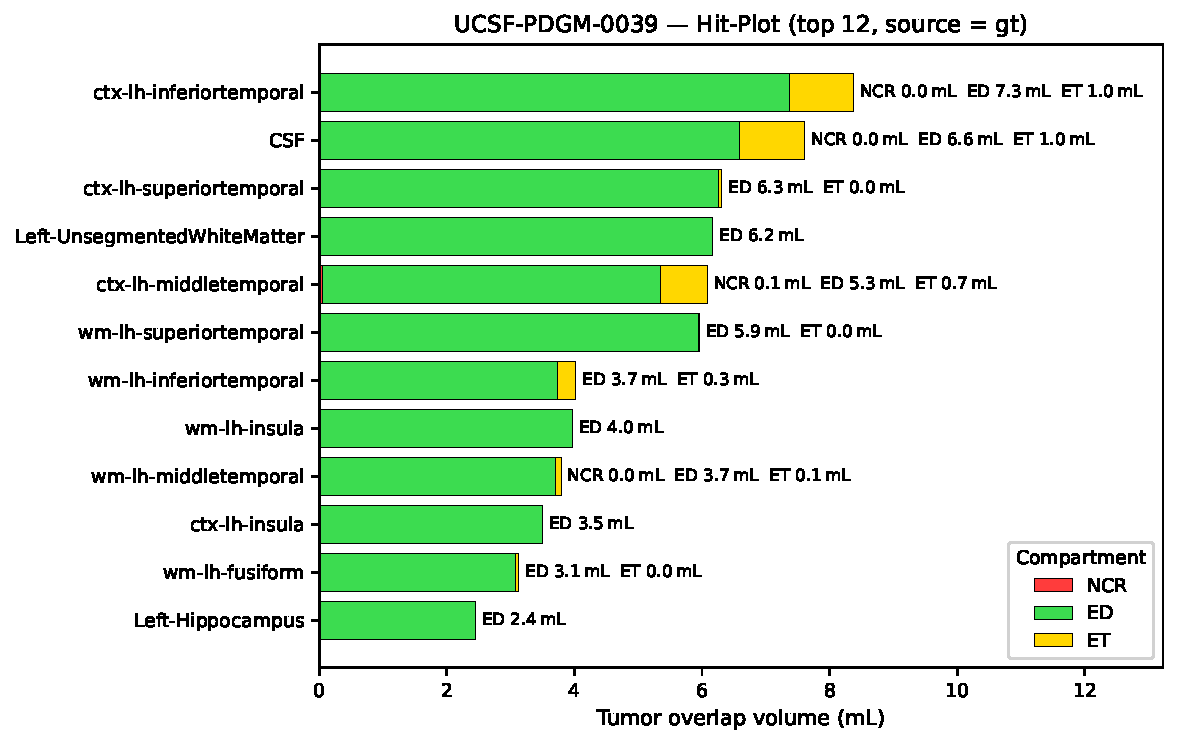
\includegraphics[width=0.88\textwidth]{figs/sub-0039_panel_i_hitplot_gt.pdf}
\end{tabular}
\vspace{-4mm}
\caption{Tumor location and anatomical neighborhoods from the study UCSF-PDGM-0039. a) The original Gadolinium-contrast enhanced T1-weighted image (T1c) with an overlay of tumor region boundaries. Insert in the left panel shows the corresponding synthesized super-resolution T1 MPRAGE image (\texttt{synthSR}) in a para-sagittal section. Insert in the middle panel, covering the tumor in a coronal section, showing the corresponding FLAIR channel.  b) The \texttt{synthseg} (not \texttt{wmparc}) segmentation with an overlay of tumor compartment boundaries and annotation of selected anatomical structures and regions in the tumor surroundings. Insert in the right panel shows the corresponding three-compartment tumor segmentation using our extended \texttt{FreeSurferTumorColorLUT} lookup table. The black crosshair center is located at [\texttt{i=167}, \texttt{j=111}, \texttt{k=45}]. Visualization of normal and abnormal tissue in the sagittal, coronal, and axial planes are made with \texttt{Freeview} and color-coded labels according to the \texttt{FreeSurferColorLUT} lookup table. c) Tumor compartment ``Hit-Plot'' for the top-12 \texttt{wmparc} parcels of this subject.}
\label{fig:UCSF-PDGM-0039_countouring}
\end{figure}

\begin{figure}[H]
\begin{tabular}{c}
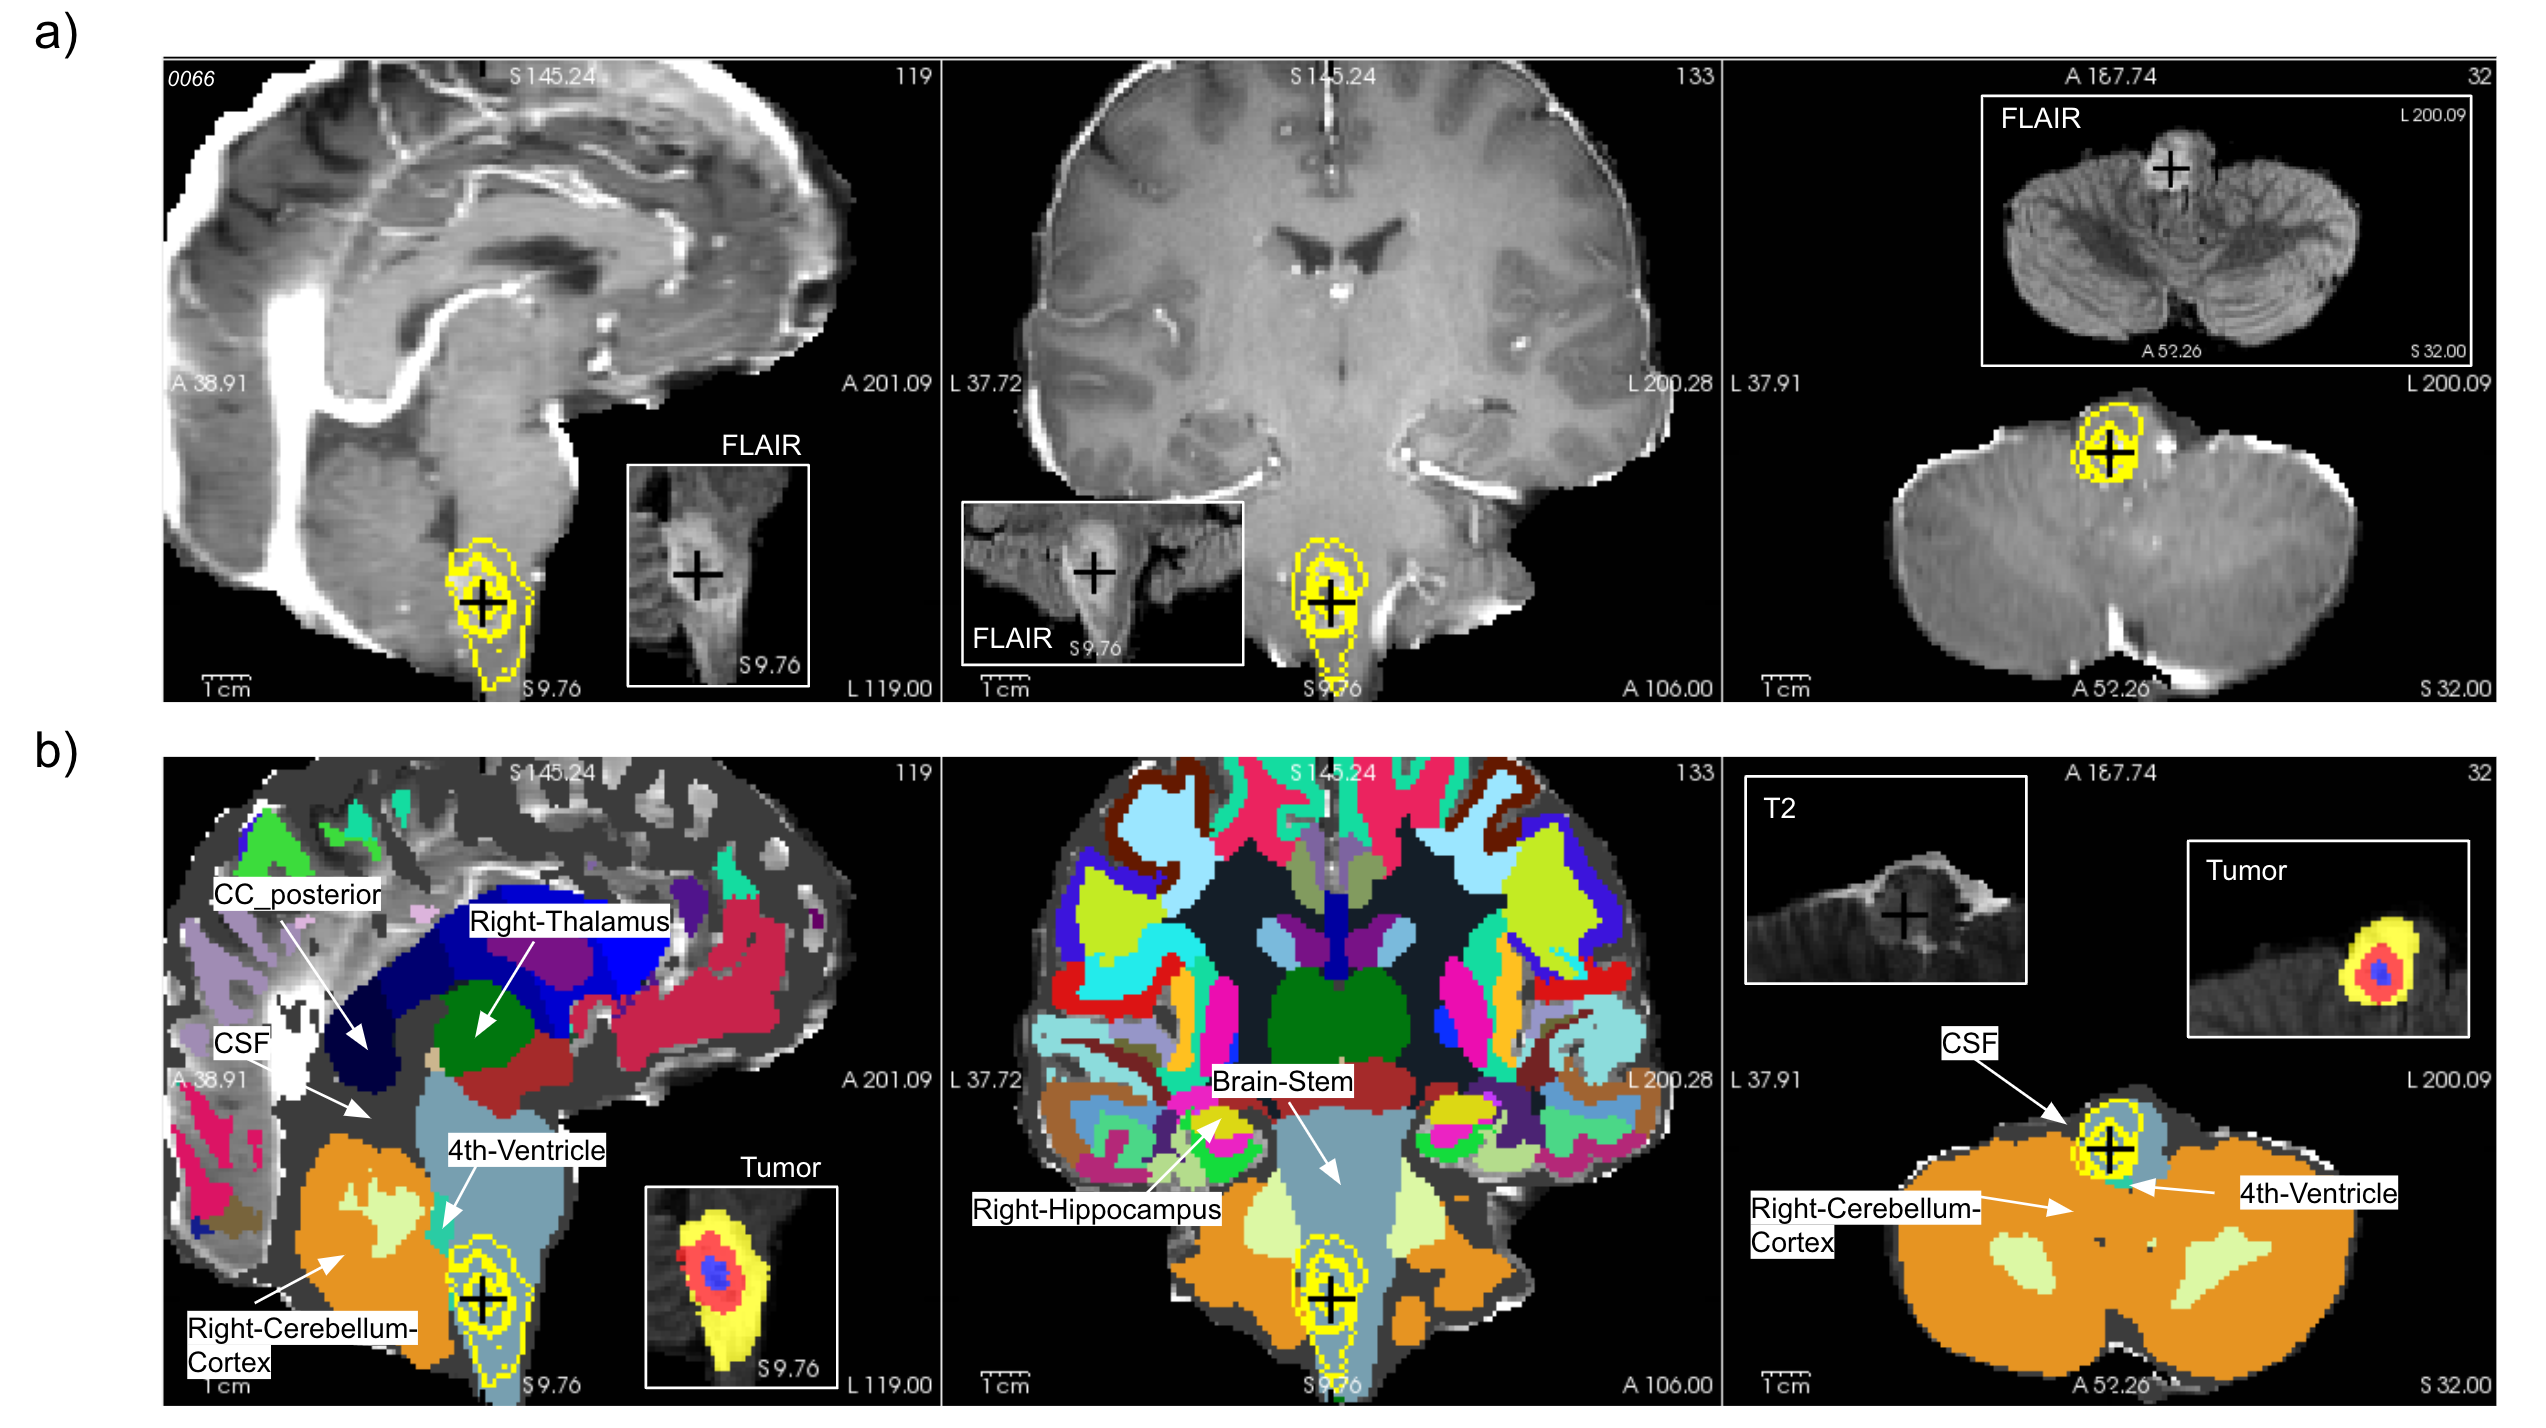
\includegraphics[width=0.84\textwidth]{figs/glioma-localization-figs-UCSF-PDGM-0066-tumor-contours-on-wmparc.png} \\
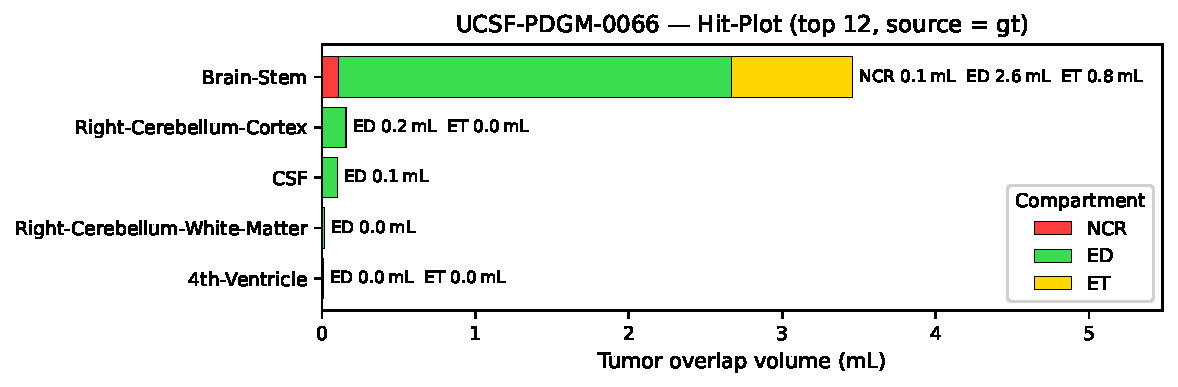
\includegraphics[width=0.84\textwidth]{figs/sub-0066_panel_i_hitplot_gt.pdf}
\end{tabular}
\vspace{-4mm}
\caption{Tumor location and anatomical neighborhoods from the study UCSF-PDGM-0066. a) The original Gadolinium-contrast enhanced T1-weighted image (T1c) with an overlay of tumor region boundaries. Inserts covering the tumor region show the corresponding FLAIR channel without the superposition of tumor region boundaries. b) The \texttt{wmparc} segmentation with an overlay of tumor compartment boundaries and annotation of selected anatomical structures and regions in the tumor surroundings. Inserts in the left and right panel show the corresponding three-compartment tumor segmentation using our extended \texttt{FreeSurferTumorColorLUT} lookup table. The right panel also shows an insert of the T2 channel with the small tumor partly surrounded by CSF. The black crosshair center is located at [\texttt{i=119}, \texttt{j=133}, \texttt{k=32}]. Visualization of normal and abnormal tissue in the sagittal, coronal, and axial planes are made with \texttt{Freeview} and color-coded labels according to the \texttt{FreeSurferColorLUT} lookup table. c) Tumor compartment ``Hit-Plot'' for the top-12 \texttt{wmparc} parcels of this subject (this small lesion is partly surrounded by CSF, which appears in the bar chart as a non-trivial CSF compartment overlap).}
\label{fig:UCSF-PDGM-0066_countouring}
\end{figure}


\begin{figure}[H]
\begin{tabular}{c}
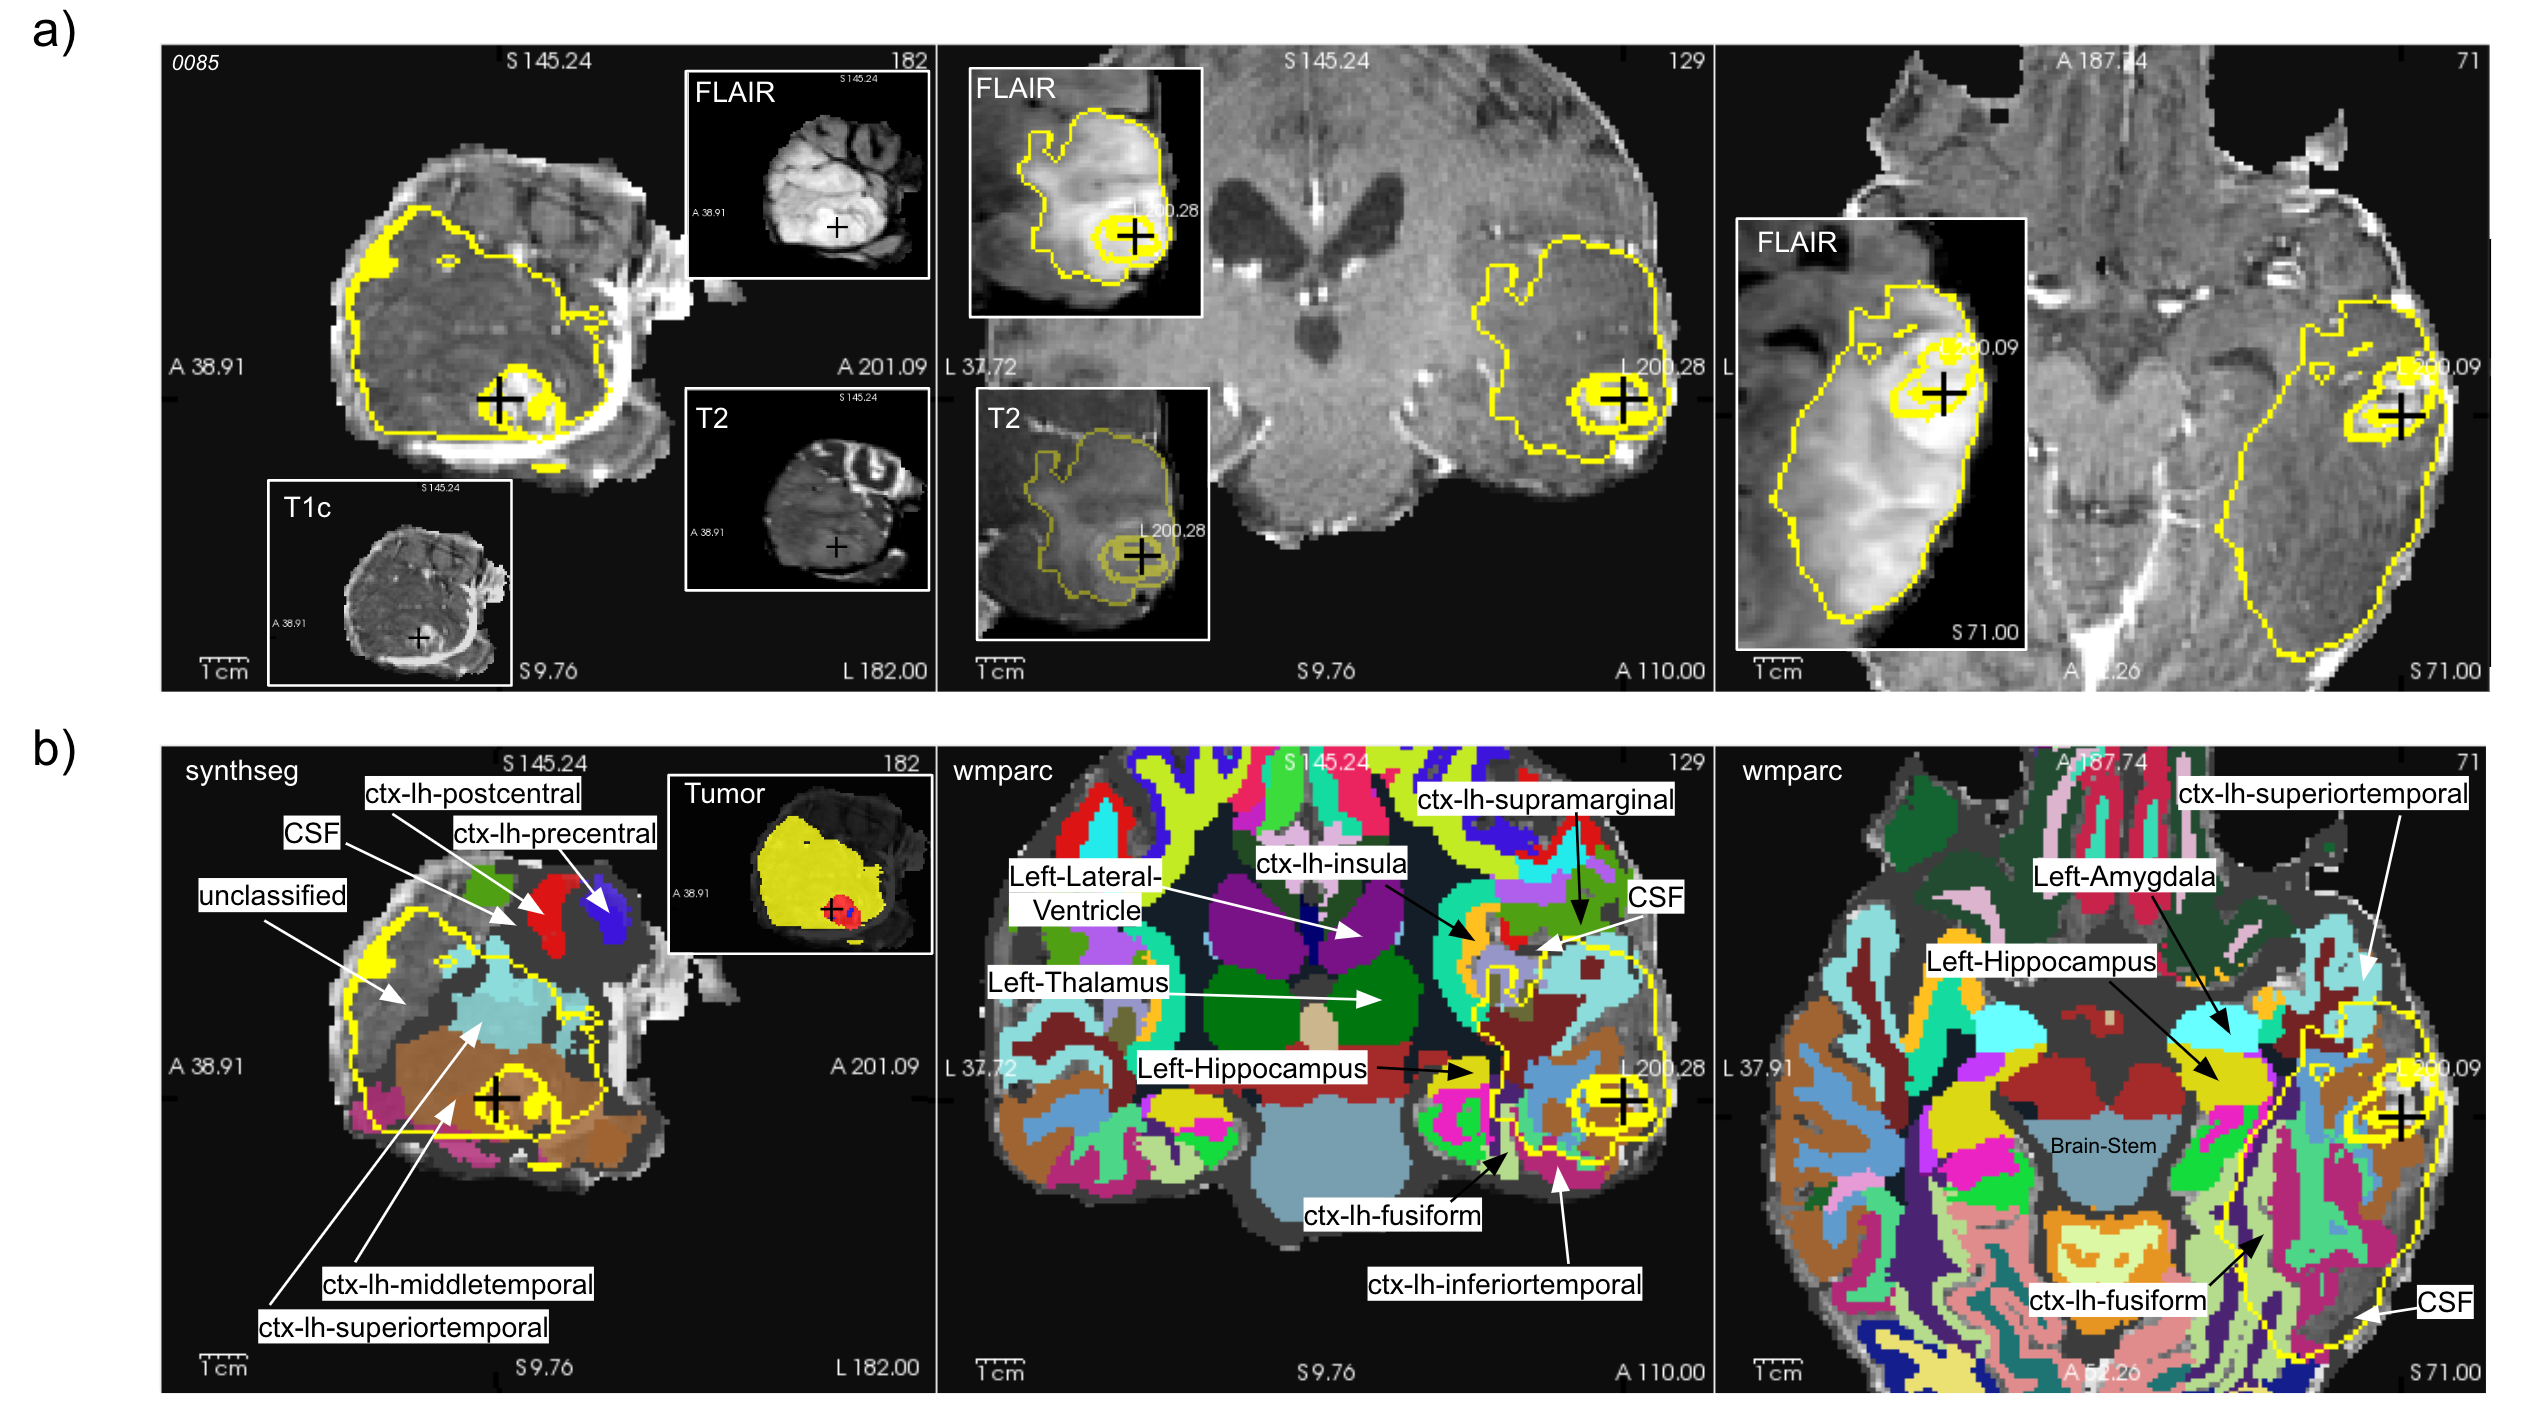
\includegraphics[width=0.72\textwidth]{figs/glioma-localization-figs-UCSF-PDGM-0085-tumor-contours-on-wmparc.png} \\
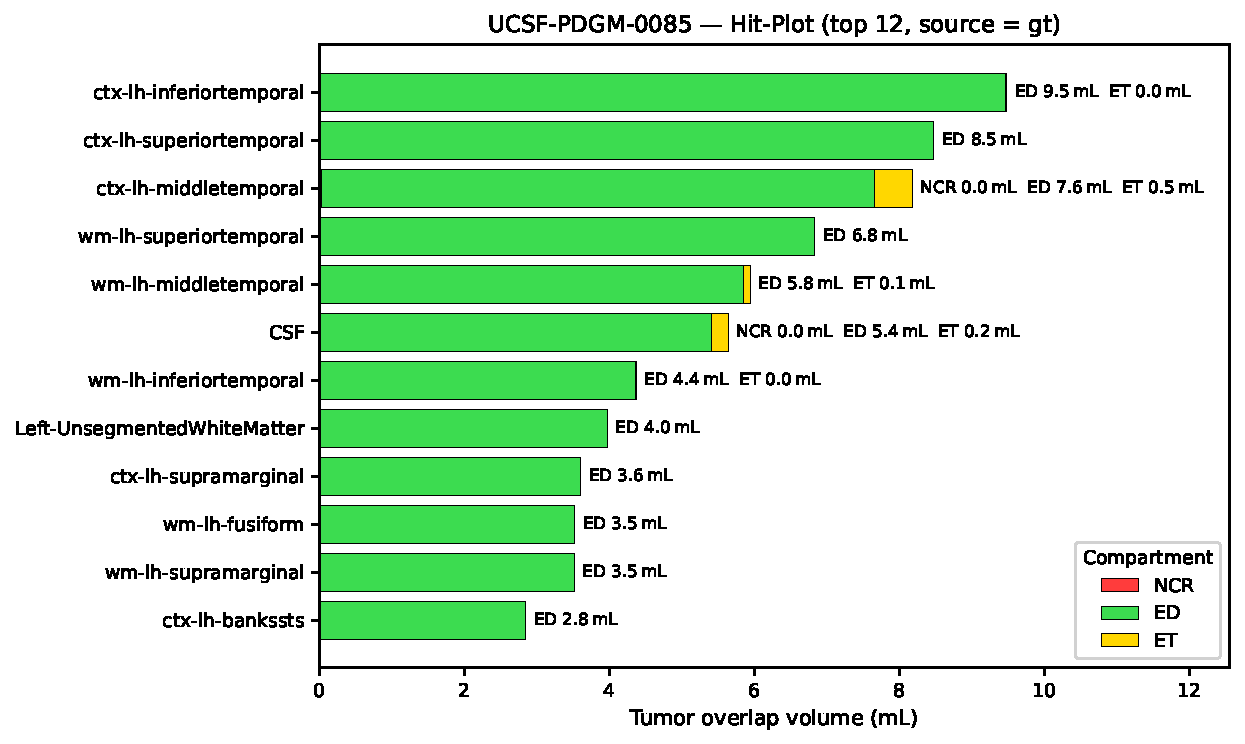
\includegraphics[width=0.66\textwidth]{figs/sub-0085_panel_i_hitplot_gt.pdf}
\end{tabular}
\vspace{-4mm}
\caption{Tumor location and anatomical neighborhoods from the study UCSF-PDGM-0085. a) The original Gadolinium-contrast enhanced T1-weighted image (T1c) with an overlay of tumor region boundaries. Insert in the right panel shows the corresponding FLAIR channel. b) The \texttt{wmparc} segmentation with an overlay of tumor compartment boundaries and annotation of selected anatomical structures and regions in the tumor surroundings. Insert in the right panel shows the corresponding three-compartment tumor segmentation using our extended \texttt{FreeSurferTumorColorLUT} lookup table. The black crosshair center is located at [\texttt{i=182}, \texttt{j=129}, \texttt{k=71}]. Visualization of normal and abnormal tissue in the sagittal, coronal, and axial planes are made with \texttt{Freeview} and color-coded labels according to the \texttt{FreeSurferColorLUT} lookup table. c) Tumor compartment ``Hit-Plot'' for the top-12 \texttt{wmparc} parcels of this subject.}
\label{fig:UCSF-PDGM-0085_countouring}
\end{figure}




\section*{\large APPENDIX 3. Per-subject DL-vs-reference Hit-Plot agreement on five representative leak-safe cohort subjects}
\label{sec:appendix-supp-dlvsgt}

The five detail subjects of \emph{APPENDIX~2} (UCSF-PDGM-0039, -0066, -0085) and Figures~\ref{fig:UCSF-PDGM-0020_countouring} and \ref{fig:UCSF-PDGM-0022_countouring} are leak-unsafe for the unified BraTS21-derived DL engine by construction (four of five sit in the BraTS21 Segmentation \emph{Training} cohort; the fifth in \emph{Validation}). To answer the per-subject form of ``how does the DL Hit-Plot compare to the reference Hit-Plot'' without violating the leak-safe evaluation paradigm, the supplementary panel below uses five \emph{representative} subjects drawn from the $n=50$ evaluation cohort (cohort manifest cited in Methods) where DL inference is legitimate test-set inference.

\paragraph{Selection rule (S-D).}
The five subjects shown are those whose mean absolute per-cell residual, averaged across all (parcel, compartment) cells of the per-cell residual table computed for Figure~\ref{fig:hitplot-agreement}, is closest to the cohort mean residual; ties are broken by subject id ascending. The pick is therefore deterministic and produces a representative slice of the cohort agreement distribution rather than a cherry-picked best/worst.

\begin{figure}[H]
\centering
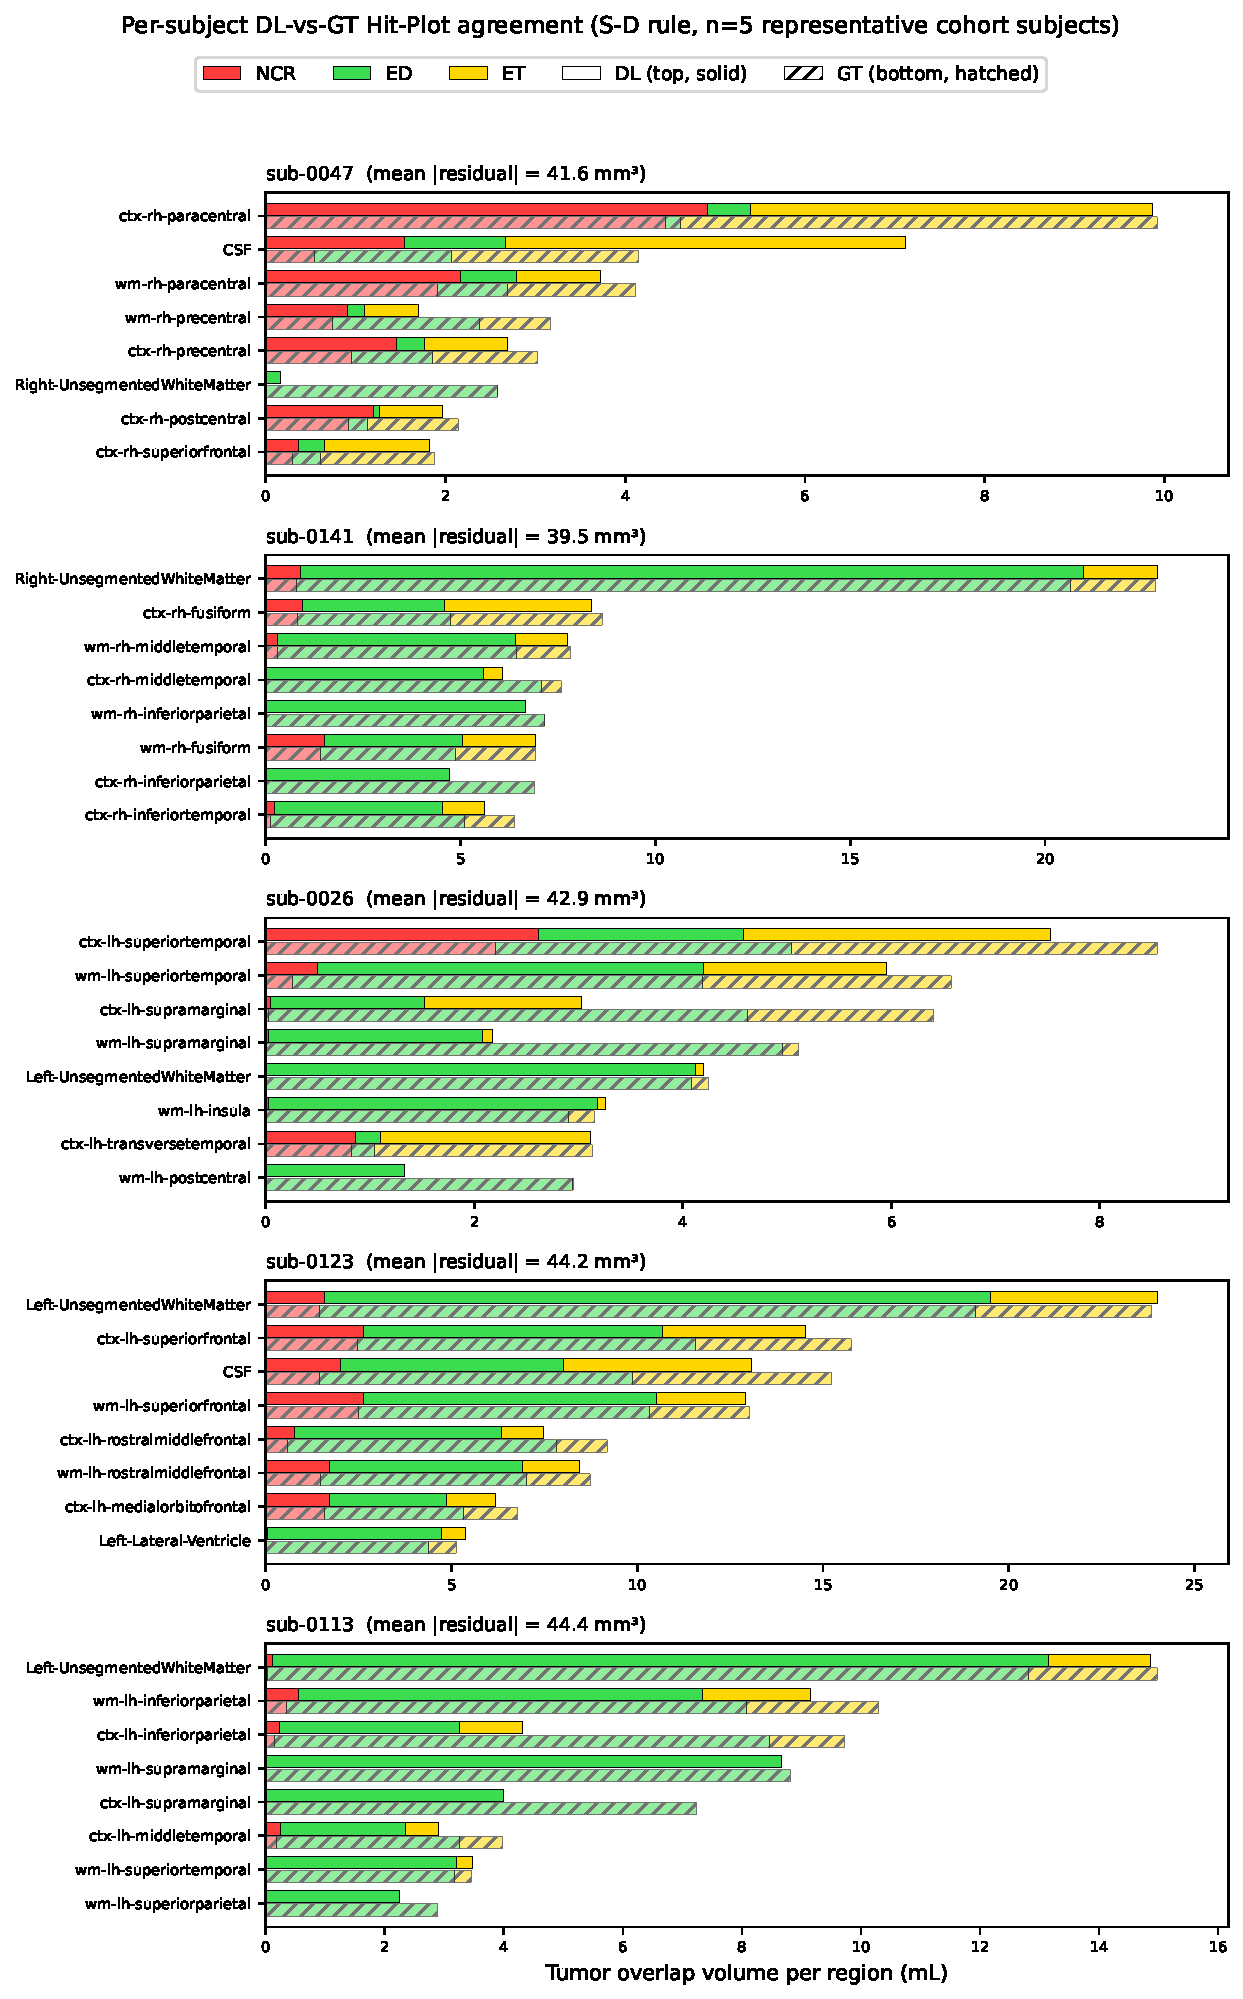
\includegraphics[width=0.78\textwidth]{figs/supp_legacy5_dlvsgt_panel.pdf}
\caption{Per-subject DL-vs-reference Hit-Plot agreement on five representative subjects from the $n=50$ evaluation cohort. Each row shows one subject; every region has two horizontal bars, the unified DL engine's Hit-Plot on top (solid colours, NCR + ED + ET stacked) and the dataset-provided reference Hit-Plot below (same colours, hatched). Top-8 \texttt{wmparc} regions per subject are shown, ranked by the maximum of DL- and reference-side total overlap volume. Subjects are picked by the deterministic S-D rule (\emph{Selection rule} above); the cohort mean absolute per-cell residual ($41.07$\,mm$^3$) and per-subject means appear in each subplot title. Compartment colours match Figure~\ref{fig:UCSF-PDGM-0020_a_h} panel~(e).}
\label{fig:supp-legacy5-dlvsgt}
\end{figure}

\section*{\large APPENDIX 4. Functional-anatomy Hit-Plot summary on the leak-safe cohort}
\label{sec:appendix-functional-anatomy-hitplot}

The panel below summarises the $n=50$ UCSF-PDGM Hit-Plot-GT
matrix after collapsing \texttt{wmparc} labels into a small set of
pre-defined anatomical groups. The top-left panel uses the full
cohort; the remaining panels repeat the same summary by OS tertile
(short, mid, long) as an exploratory stratified view.

\begin{figure}[H]
\centering
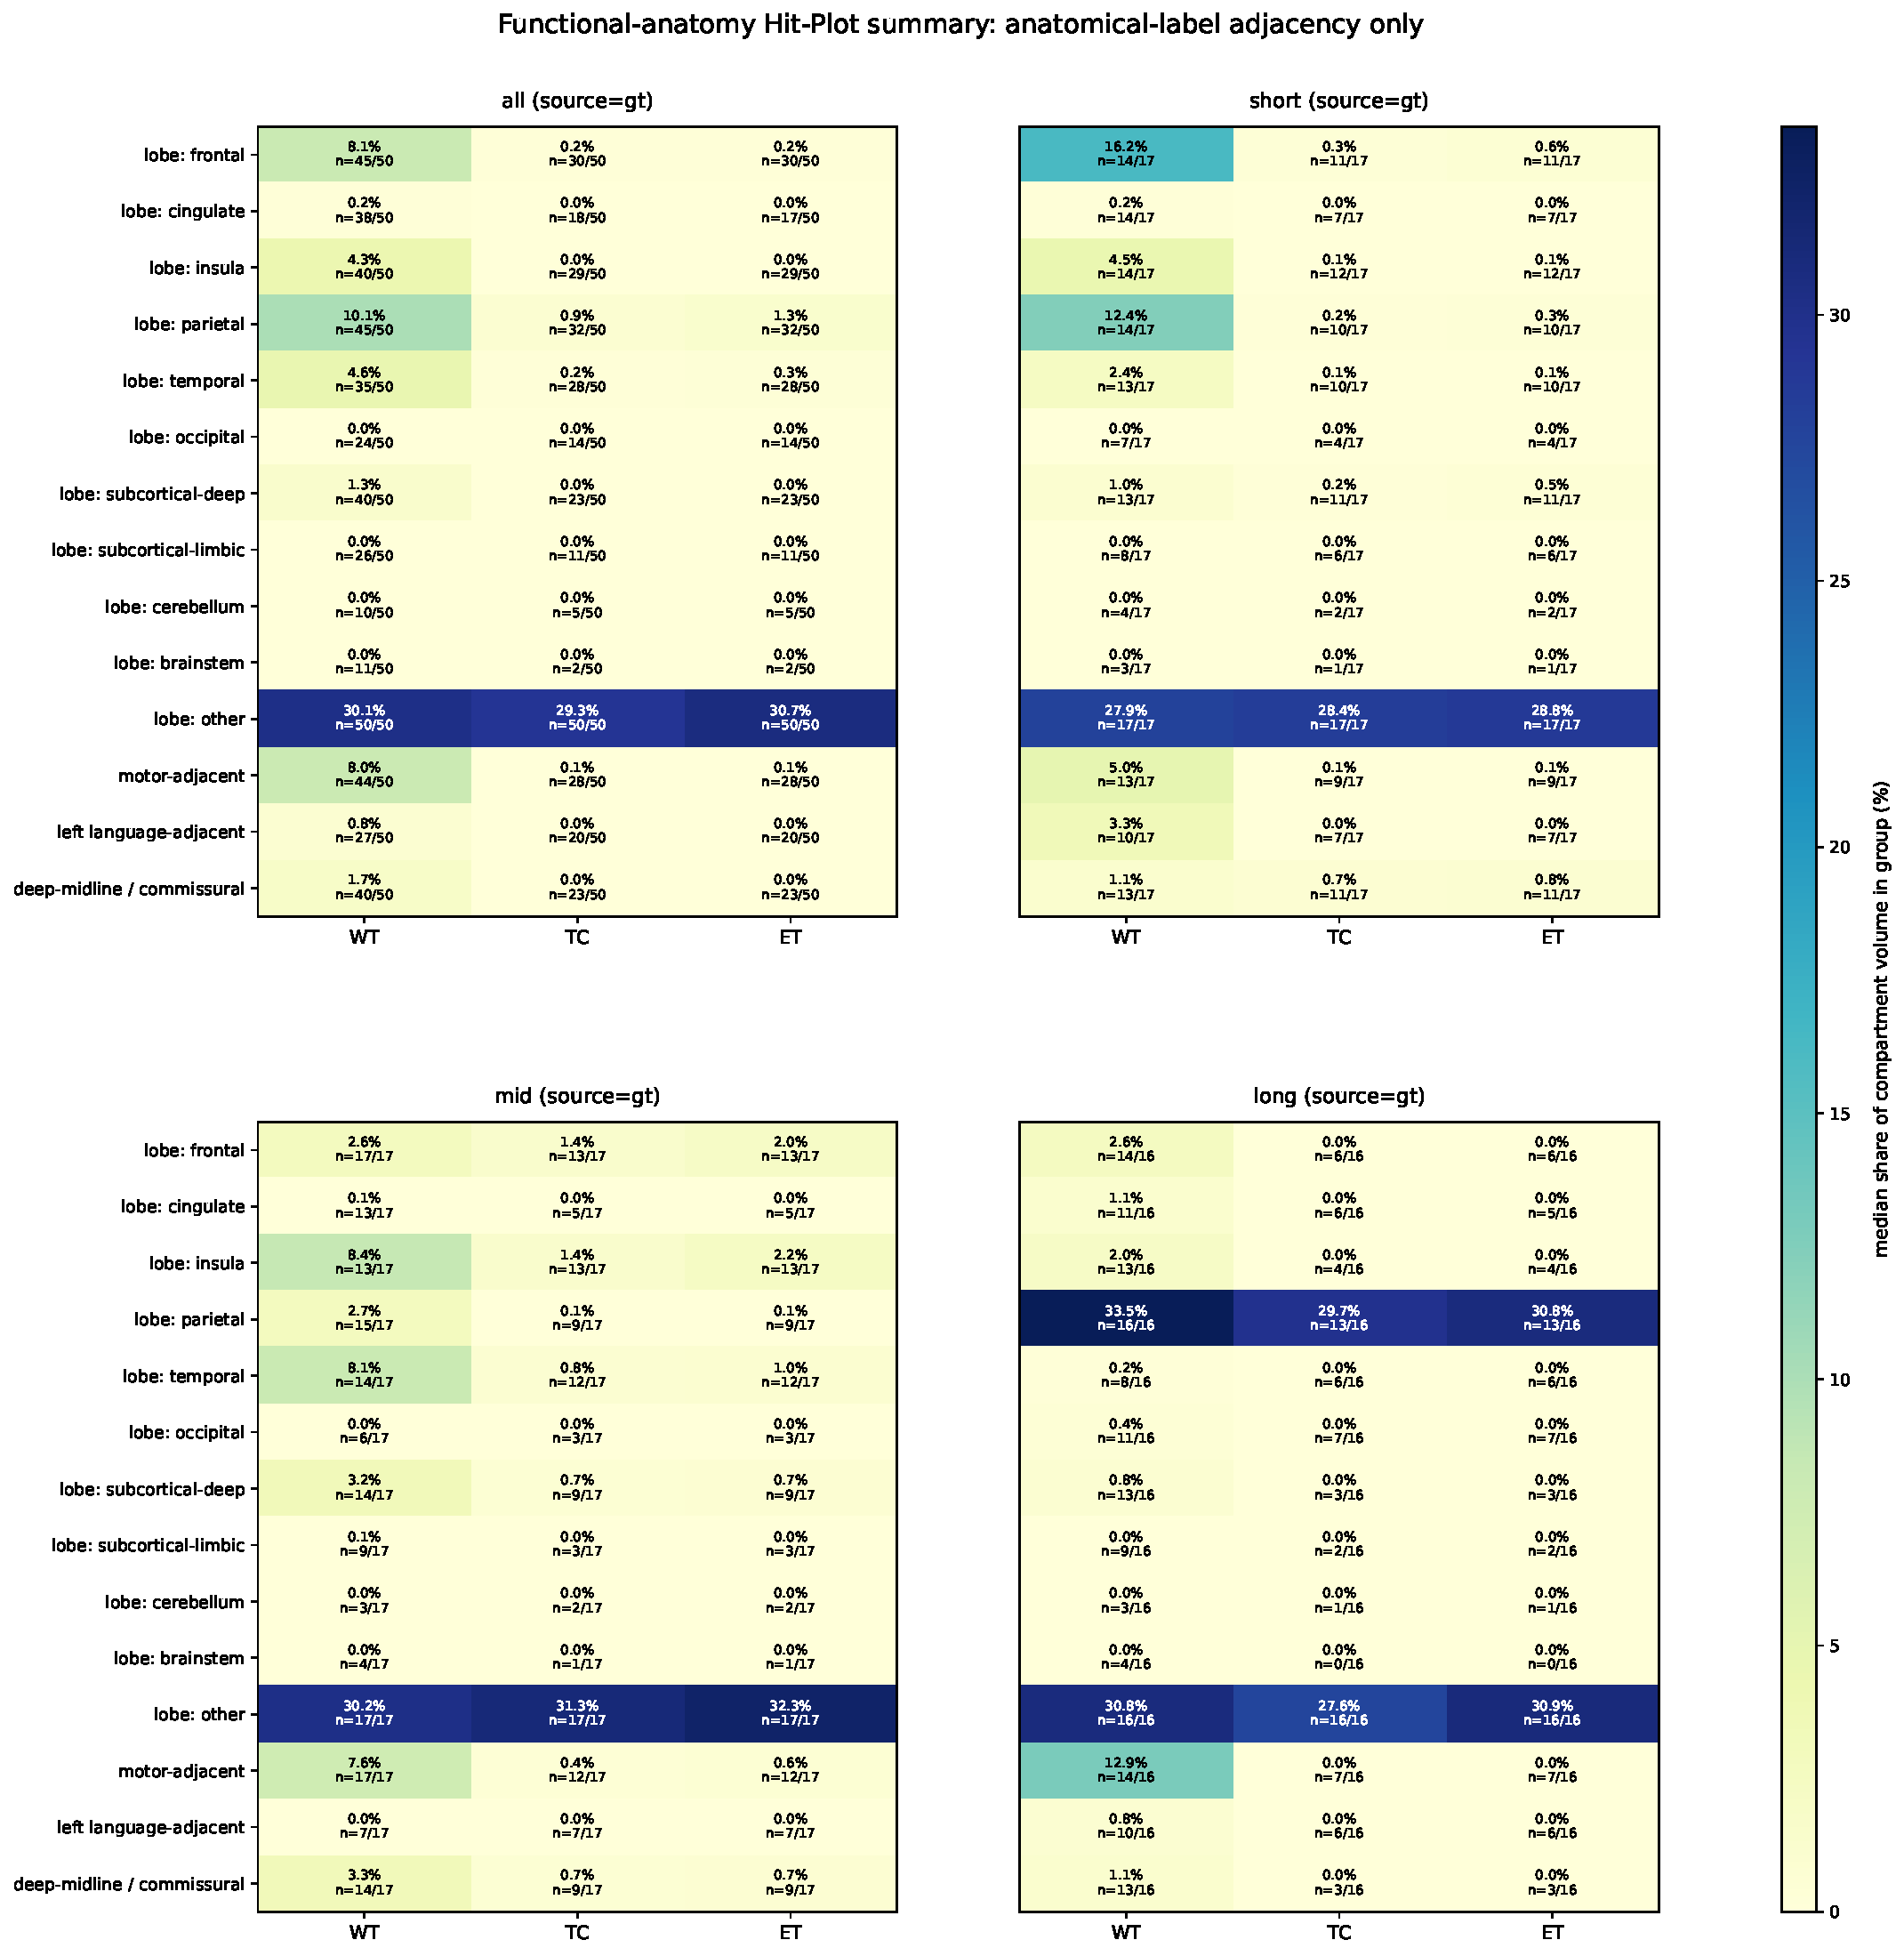
\includegraphics[width=0.90\textwidth]{figs/fig_functional_anatomy_hitplot_gt.pdf}
\caption{\textbf{Functional-anatomy summary of the Hit-Plot on
the leak-safe UCSF-PDGM cohort.} Rows are pre-defined
\texttt{wmparc}-derived groups: the existing lobar bins plus three
anatomical-label adjacency summaries (motor-adjacent, left
language-adjacent, and deep-midline / commissural). Columns are BraTS
compartments (WT, TC, ET). Cell colour gives the median share of the
compartment volume falling in that group; text gives the median
percentage and the prevalence denominator $n=K/N$ for any overlap in
the group. The figure is generated from the existing per-subject
Hit-Plot CSVs and \texttt{wmparc} LUT sidecars; a companion DL
sensitivity run gives similar all-cohort WT summaries (motor-adjacent
$43/50$, median $6.91\,\%$; left language-adjacent $27/50$, median
$0.71\,\%$; deep-midline / commissural $42/50$, median $2.06\,\%$).
These groups are anatomical-label adjacency summaries only: they are
not tractography, individualized eloquence mapping, fMRI, organ-at-risk
proximity, treatment-planning validation, or outcome prediction.}
\label{fig:functional-anatomy-hitplot}
\end{figure}

\enlargethispage{\baselineskip}
\noindent \textit{Interpretation.} Appendix~4 collapses
high-dimensional Hit-Plots into readable anatomical-label groups while
preserving their descriptive role: WT commonly involves
motor-adjacent and deep-midline / commissural groups, whereas left
language-adjacent overlap is lower-burden; OS-tertile panels are a
readability check, not an outcome-association test.

\section*{\large APPENDIX 5. TumorSynth sensitivity analysis of the functional-anatomy Hit-Plot}
\label{sec:appendix-tumorsynth-functional-anatomy-hitplot}

The table and panels below repeat the Appendix~4 cohort-level
Hit-Plot summaries after replacing the MONAI~Bundle BraTS
three-compartment SegResNet masks with \texttt{mri\_TumorSynth} /
nnU-Net~v1.7 masks generated for all $50/50$ leak-safe UCSF-PDGM
subjects. TumorSynth here runs on the same staged mpMRI inputs as the MONAI~Bundle, rather than the SRI-24-registered, skull-stripped volumes it expects; the comparison below is therefore a bounded check on backbone sensitivity, and should not beread as a best-case TumorSynth benchmark.

\begin{table}[H]
\centering
\caption{\textbf{Voxel-space agreement between the unified
MONAI~Bundle segmentation and the \texttt{mri\_TumorSynth} sensitivity
run on the $n=50$ UCSF-PDGM cohort.} Values are median [Q1, Q3] over
subjects for the paired comparison DL vs.\ TumorSynth, using the same
WT, TC, and ET compartment definitions as Table~\ref{table:dl-vs-gt}.
The comparison is input-matched to the HPGS staged mpMRI files and is
therefore interpreted as a bounded segmentation-backbone sensitivity
analysis.}
\label{table:tumorsynth-agreement}
\begin{tabular}{l c c c}
\toprule
Metric & WT & TC & ET \\
\midrule
Dice & 0.894 [0.866, 0.921] & 0.860 [0.793, 0.901] & 0.672 [0.559, 0.736] \\
HD$_{95}$ (mm) & 4.06 [3.20, 5.83] & 4.30 [3.04, 6.38] & 4.00 [3.00, 5.39] \\
$|\mathrm{VE}|$ (mm$^3$) & 6544 [3547, 12452] & 2652 [906, 6561] & 3704 [793, 7590] \\
Sensitivity & 0.878 [0.831, 0.914] & 0.894 [0.777, 0.946] & 0.660 [0.507, 0.762] \\
Specificity & 1.000 [0.999, 1.000] & 1.000 [0.999, 1.000] & 1.000 [0.999, 1.000] \\
\bottomrule
\end{tabular}

\end{table}

\begin{figure}[H]
\centering
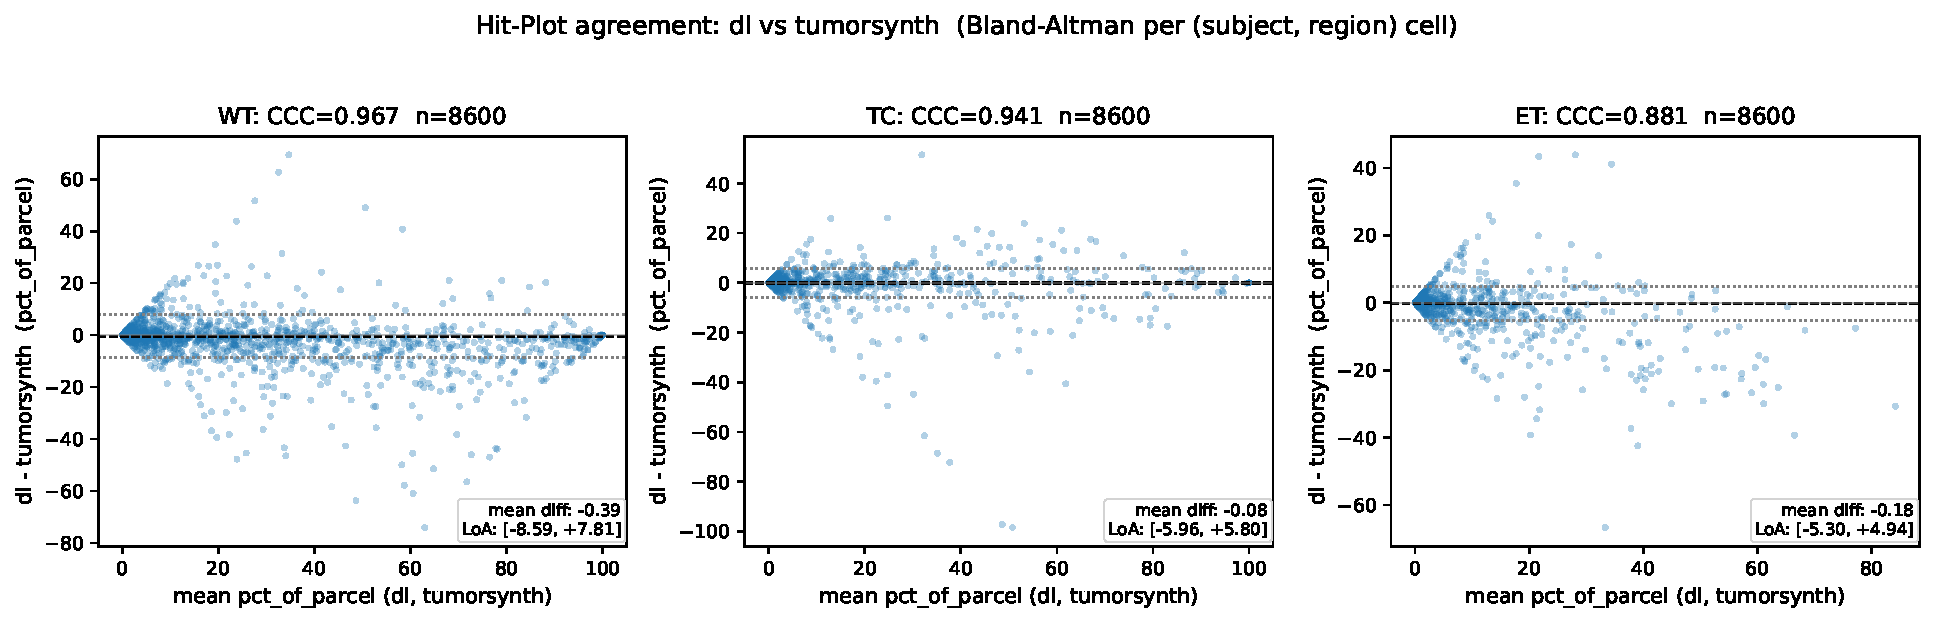
\includegraphics[width=0.90\textwidth]{figs/fig_hitplot_agreement_dl_vs_tumorsynth.pdf}
\caption{\textbf{Cell-level Hit-Plot agreement between the
unified MONAI~Bundle segmentation and \texttt{mri\_TumorSynth}.}
Each point is one subject-by-\texttt{wmparc}-region cell
($50\times172=8\,600$ cells per compartment). Bland-Altman summaries
compare the DL and TumorSynth Hit-Plot percentage of parcel volume for
WT, TC, and ET. Concordance remains high at the anatomical-profile
level (CCC $0.967$ WT, $0.941$ TC, $0.881$ ET), with mean differences
of $-0.39$, $-0.08$, and $-0.18$ percentage points of parcel volume,
respectively.}
\label{fig:hitplot-agreement-dl-vs-tumorsynth}
\end{figure}

\begin{figure}[H]
\centering
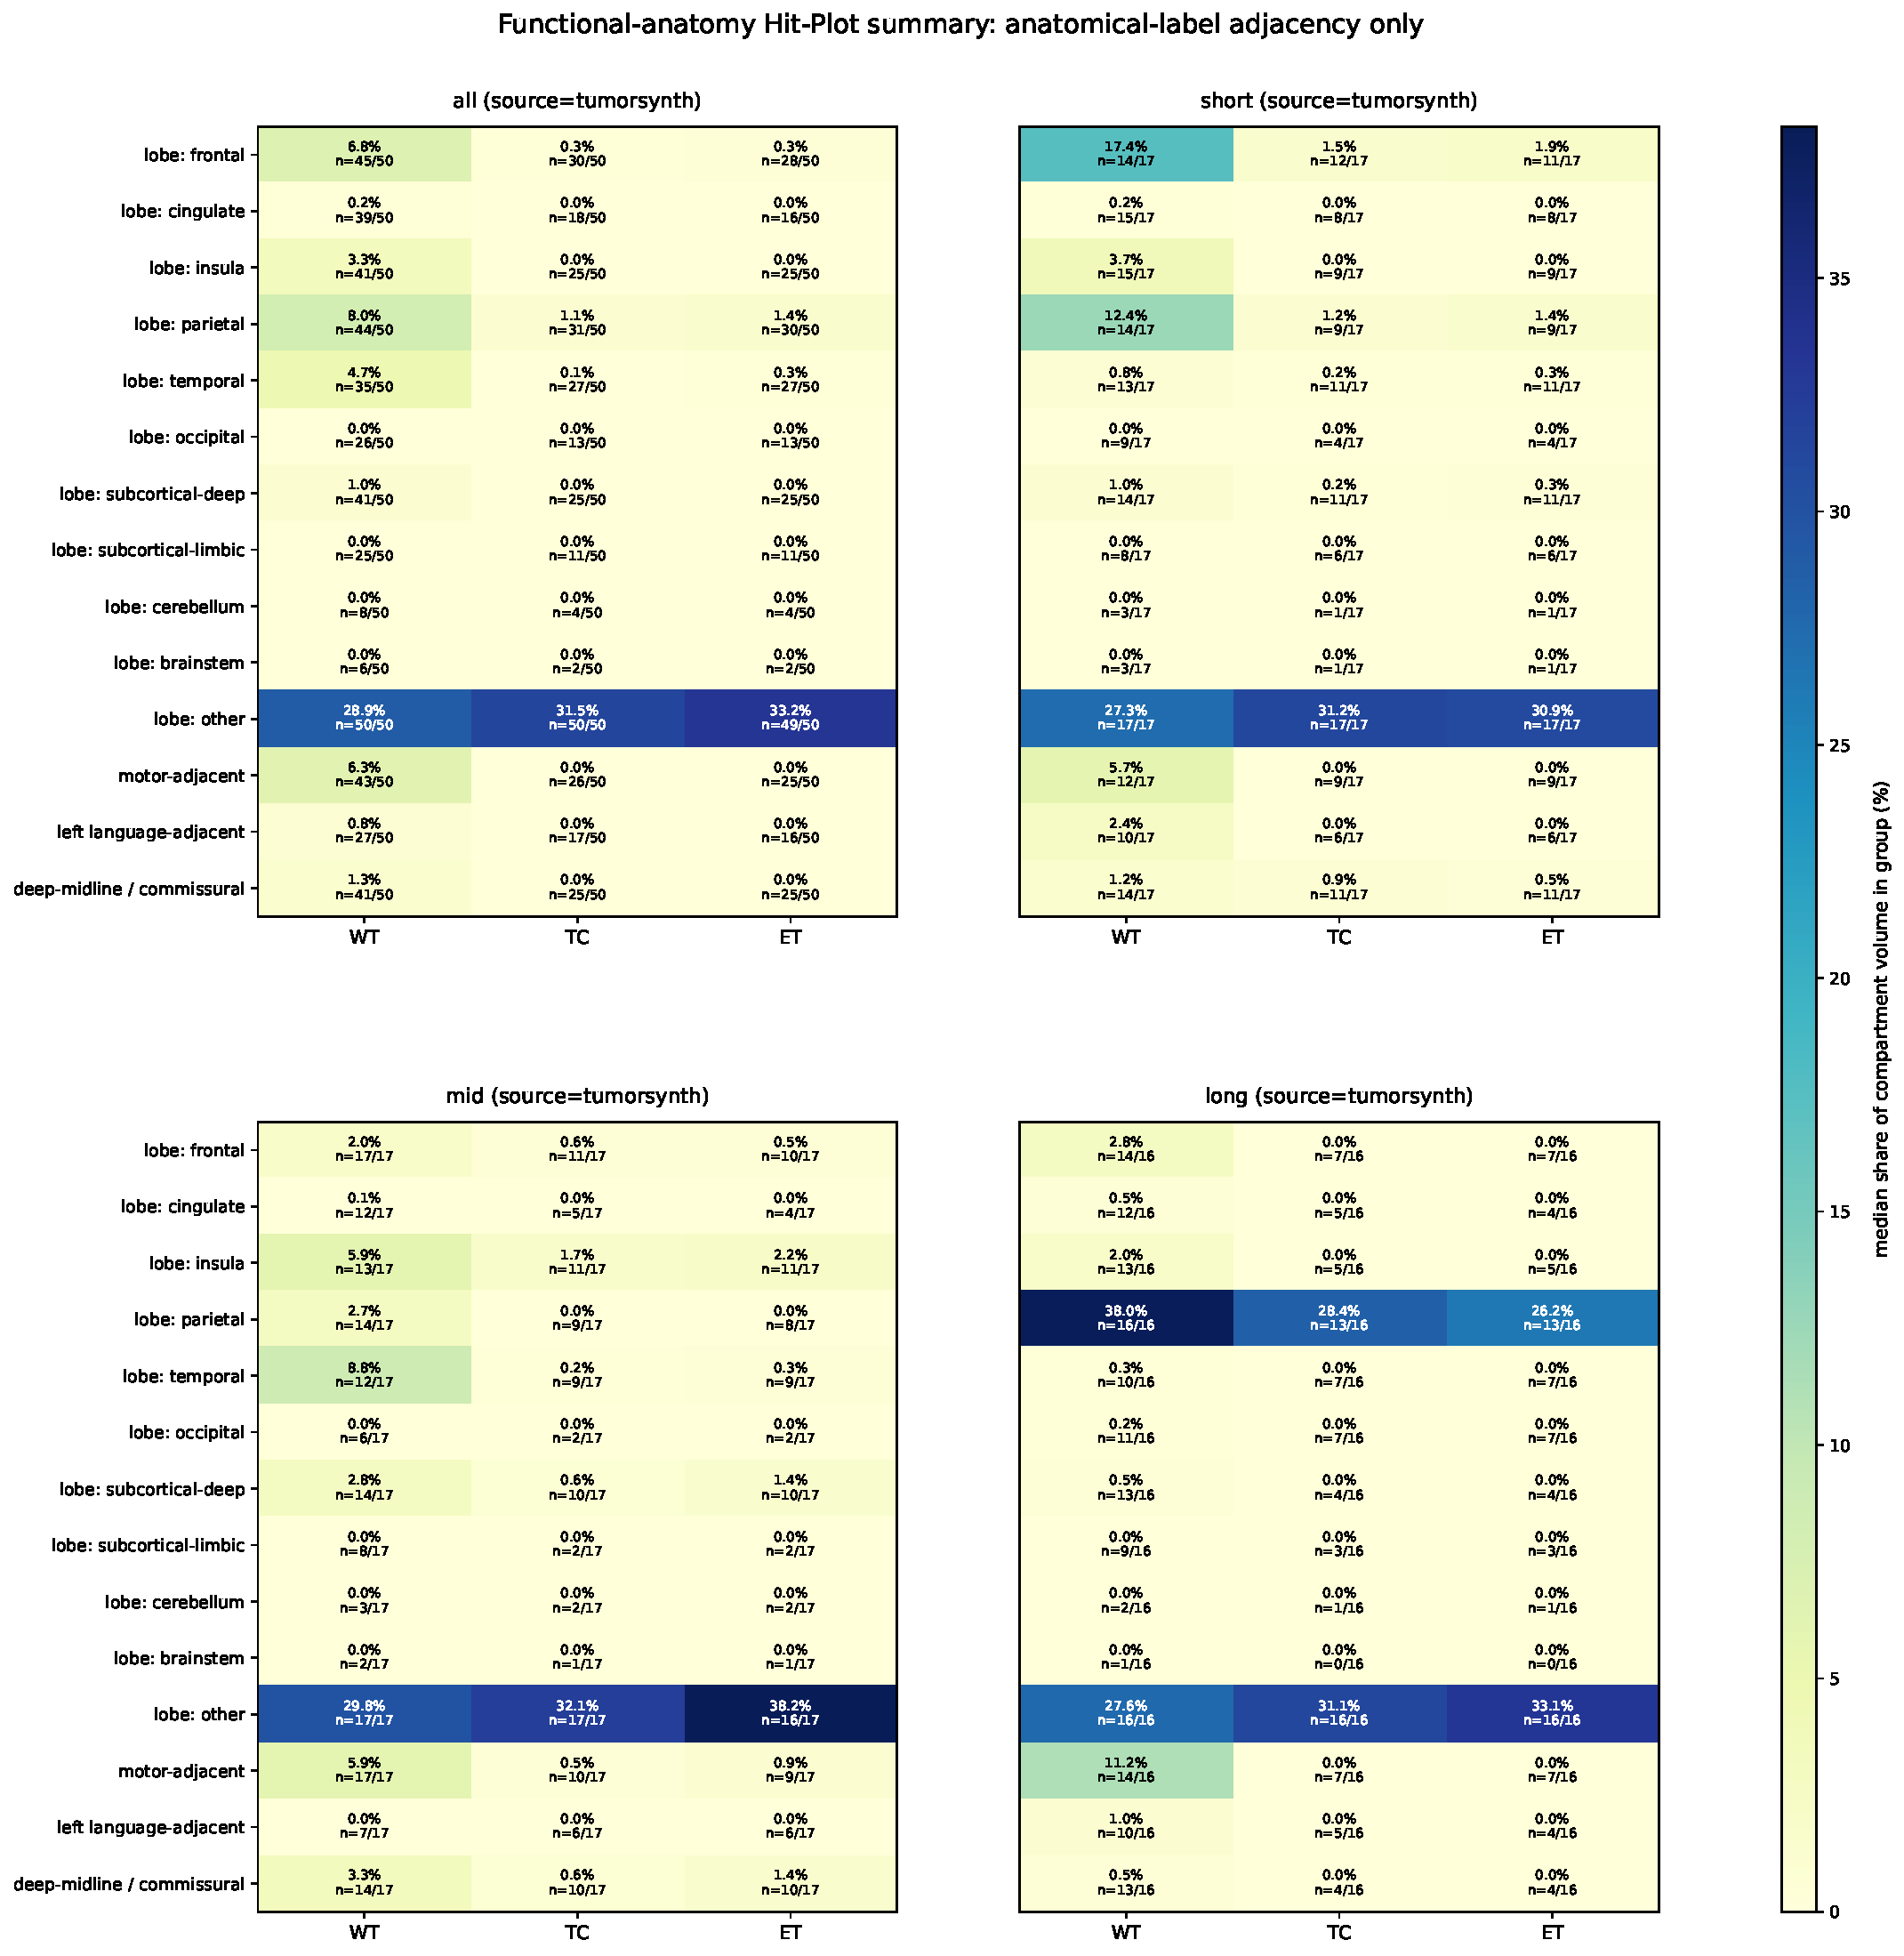
\includegraphics[width=0.90\textwidth]{figs/fig_functional_anatomy_hitplot_tumorsynth.pdf}
\caption{\textbf{Functional-anatomy summary of the
\texttt{mri\_TumorSynth}-driven Hit-Plot on the leak-safe UCSF-PDGM
cohort.} The layout, groups, and cell semantics match
Figure~\ref{fig:functional-anatomy-hitplot}: rows are pre-defined
\texttt{wmparc}-derived lobar and anatomical-label adjacency groups;
columns are WT, TC, and ET; colour gives the median share of
compartment volume in the group; text gives median percentage and
prevalence $n=K/N$. The all-cohort WT summaries remain close to the
reference-mask and MONAI~Bundle summaries in Appendix~4
(motor-adjacent $43/50$, median $6.27\,\%$; left language-adjacent
$27/50$, median $0.84\,\%$; deep-midline / commissural $41/50$,
median $1.28\,\%$), while voxel-space ET agreement is more variable
(Table~\ref{table:tumorsynth-agreement}). This supports the use of
the Hit-Plot as a readable anatomy-aware summary while
preserving the methodological caveat that TumorSynth was not run under
its ideal SRI-24-registered preprocessing regime.}
\label{fig:functional-anatomy-hitplot-tumorsynth}
\end{figure}

\noindent \textit{Interpretation.} Appendix~5 shows that the
cohort-level anatomical profile is broadly preserved after swapping
the segmentation backbone from the MONAI~Bundle model to
\texttt{mri\_TumorSynth}: voxel-space agreement is strongest for WT
and TC and weaker for ET, but the cell-level Hit-Plot concordance
remains high and the functional-anatomy WT summaries retain the same
qualitative pattern. We therefore interpret the appendix as evidence
that the descriptive regional profile is reasonably stable to this
bounded backbone perturbation, while maintaining the caveat that
TumorSynth was not run under its ideal SRI-24 preprocessing regime.




\end{document}
